% Options for packages loaded elsewhere
\PassOptionsToPackage{unicode}{hyperref}
\PassOptionsToPackage{hyphens}{url}
%
\documentclass[
  openany]{book}
\usepackage{amsmath,amssymb}
\usepackage{lmodern}
\usepackage{ifxetex,ifluatex}
\ifnum 0\ifxetex 1\fi\ifluatex 1\fi=0 % if pdftex
  \usepackage[T1]{fontenc}
  \usepackage[utf8]{inputenc}
  \usepackage{textcomp} % provide euro and other symbols
\else % if luatex or xetex
  \usepackage{unicode-math}
  \defaultfontfeatures{Scale=MatchLowercase}
  \defaultfontfeatures[\rmfamily]{Ligatures=TeX,Scale=1}
\fi
% Use upquote if available, for straight quotes in verbatim environments
\IfFileExists{upquote.sty}{\usepackage{upquote}}{}
\IfFileExists{microtype.sty}{% use microtype if available
  \usepackage[]{microtype}
  \UseMicrotypeSet[protrusion]{basicmath} % disable protrusion for tt fonts
}{}
\makeatletter
\@ifundefined{KOMAClassName}{% if non-KOMA class
  \IfFileExists{parskip.sty}{%
    \usepackage{parskip}
  }{% else
    \setlength{\parindent}{0pt}
    \setlength{\parskip}{6pt plus 2pt minus 1pt}}
}{% if KOMA class
  \KOMAoptions{parskip=half}}
\makeatother
\usepackage{xcolor}
\IfFileExists{xurl.sty}{\usepackage{xurl}}{} % add URL line breaks if available
\IfFileExists{bookmark.sty}{\usepackage{bookmark}}{\usepackage{hyperref}}
\hypersetup{
  pdftitle={Large-scale compositional analysis of invertebrate viromes estimated from public RNA-Seq data},
  pdfauthor={Pau Alfonso i Comos},
  hidelinks,
  pdfcreator={LaTeX via pandoc}}
\urlstyle{same} % disable monospaced font for URLs
\usepackage{longtable,booktabs,array}
\usepackage{calc} % for calculating minipage widths
% Correct order of tables after \paragraph or \subparagraph
\usepackage{etoolbox}
\makeatletter
\patchcmd\longtable{\par}{\if@noskipsec\mbox{}\fi\par}{}{}
\makeatother
% Allow footnotes in longtable head/foot
\IfFileExists{footnotehyper.sty}{\usepackage{footnotehyper}}{\usepackage{footnote}}
\makesavenoteenv{longtable}
\usepackage{graphicx}
\makeatletter
\def\maxwidth{\ifdim\Gin@nat@width>\linewidth\linewidth\else\Gin@nat@width\fi}
\def\maxheight{\ifdim\Gin@nat@height>\textheight\textheight\else\Gin@nat@height\fi}
\makeatother
% Scale images if necessary, so that they will not overflow the page
% margins by default, and it is still possible to overwrite the defaults
% using explicit options in \includegraphics[width, height, ...]{}
\setkeys{Gin}{width=\maxwidth,height=\maxheight,keepaspectratio}
% Set default figure placement to htbp
\makeatletter
\def\fps@figure{htbp}
\makeatother
\setlength{\emergencystretch}{3em} % prevent overfull lines
\providecommand{\tightlist}{%
  \setlength{\itemsep}{0pt}\setlength{\parskip}{0pt}}
\setcounter{secnumdepth}{5}
\usepackage{booktabs}
\AtBeginDocument{\renewcommand{\chaptername}{Part}}
\usepackage{booktabs}
\usepackage{longtable}
\usepackage{array}
\usepackage{multirow}
\usepackage{wrapfig}
\usepackage{float}
\usepackage{colortbl}
\usepackage{pdflscape}
\usepackage{tabu}
\usepackage{threeparttable}
\usepackage{threeparttablex}
\usepackage[normalem]{ulem}
\usepackage{makecell}
\usepackage{hyperref}
\usepackage{float}
\usepackage{amsmath}
\usepackage{booktabs}
\usepackage{longtable}
\usepackage{array}
\usepackage{multirow}
\usepackage{wrapfig}
\usepackage{float}
\usepackage{colortbl}
\usepackage{pdflscape}
\usepackage{tabu}
\usepackage{threeparttable}
\usepackage{threeparttablex}
\usepackage[normalem]{ulem}
\usepackage{makecell}
\usepackage{xcolor}
\ifluatex
  \usepackage{selnolig}  % disable illegal ligatures
\fi
\usepackage[]{biblatex}
\addbibresource{book.bib}
\addbibresource{packages.bib}

\title{Large-scale compositional analysis of invertebrate viromes estimated from public RNA-Seq data}
\author{Pau Alfonso i Comos}
\date{July, 2022}

\begin{document}
\maketitle

{
\setcounter{tocdepth}{1}
\tableofcontents
}
\listoftables
\listoffigures
\hypertarget{acknowledgements}{%
\chapter*{Acknowledgements}\label{acknowledgements}}
\addcontentsline{toc}{chapter}{Acknowledgements}

I would like to thank LIFE-HUB.CSIC Network for providing financial support to my involvement in this project. Also, thanks to Doctors Rosa Fernández (IBE) and Ana Riesgo (MNCN) for kindly sharing their transcriptomic data with us.

I would also like to express my gratitude to Professor Santiago F. Elena for counting on me for this project and accepting me once again in his laboratory, apart from reviewing this document. I would also like to extend my thanks to everyone in the Evolutionary Systems Virology group of the Institute for Integrative Systems Biology (I\(^2\)SysBio) for sharing insightful comments and appreciations about this project with me.

The development of bioinformatic methods would not have been possible without the help of Doctor Anamarija Butković, to whom I hereby express my deepest gratitude. Also, thanks for the first revisions of this document.

I am also thankful to Professor Francisco J. Santonja for his supervision over the statistical methodologies and his recommendations on bibliography, especially at the starting point of the project.

Thanks to my parents and grandmother for supporting me in all the ways possible through all my years of study. \emph{Vos vullc}.

\hypertarget{abstract}{%
\chapter*{Abstract}\label{abstract}}
\addcontentsline{toc}{chapter}{Abstract}

Current knowledge on the viruses that coexist with invertebrates is very limited and biased towards clades of interest. The application of (meta)viromics pipelines over genomics or transcriptomics sequencing data allows for a large-scale identification of the viruses present in the sequenced sample. Metaviromics has been applied recently to some phyla of invertebrates in order to characterize their viromes, but viromes of certain phyla have been left unexplored to present date. In this study, publicly accessible transcriptomics data of very diverse invertebrate species has been used to discover how phylum and habitat affiliations shape their associated community of RNA and DNA viruses.

To achieve this goal, the development and selection of a bioinformatics pipeline for the analysis of viromes in transcriptomics data was conducted. The resulting virome compositions at a family level are set to be analyzed with compositional data analysis methods. Centered logratio (\emph{clr}) transformations are used to transform the compositions from closed data to open data so as to apply statistical multivariate methods such as PCA. It was found that invertebrate phylum can explain around \(30\%\) of the total variance in the estimated virome compositions, whereas habitat did not have such a significant impact. Overall, the identified viral families and the abundance of their transcripts were surprisingly stable among the different phyla and the viromes were dominated by transcripts of DNA viruses.

\hypertarget{introduction}{%
\chapter{Introduction}\label{introduction}}

The aim of this study is to describe the diversity of viruses associated with invertebrates based on high-throughput sequencing data analysis. Before focusing on the details of the study, let us introduce viruses, invertebrates and the basis of massive sequencing.

\hypertarget{viruses}{%
\section{Viruses}\label{viruses}}

\hypertarget{historical-insights-on-the-definition-of-a-virus}{%
\subsection{Historical insights on the definition of a virus}\label{historical-insights-on-the-definition-of-a-virus}}

The word `virus' has been used for hundreds of years as a broad term to refer to the causal agents of infectious diseases. In the late 19th century, the first hints of pathogens smaller than bacteria were found, just a few years after the works of Louis Pasteur and Robert Koch that led to a revolution in microbiology and to the proposal of the germ theory, which originally stated that microorganisms are the causal agents of infectious diseases. In this context, different authors found that the pathogens involved in infectious diseases they were studying failed to satisfy the praised criteria of Koch's postulates, because of the inability of viruses to replicate \emph{ex vivo}.

In the field of plant pathology, Martinus Beijerinck's findings regarding his research on tobacco mosaic disease published in 1898 can be considered the seed for the later development of virology, as he was convinced he was dealing with an infectious agent different in nature to microbes \autocite{Bos1999}. Among his conclusions about the newly discovered pathogen, i.e.~the tobacco mosaic virus, distinctive characteristics of viruses stand out: \emph{(i)} the infectious agent is smaller than any known bacteria, as it cannot be retained with a Chamberland filter, which were thought to not let bacteria pass through at the time, \emph{(ii)} it is unable to grow in artificial solid media, but isolates from diseased tissues remain infectious even after a few months, \emph{(iii)} it relies on the host's active metabolism to reproduce.

Parallelly with Beijernick's discoveries, the results published by Friedrich Loeffler and Paul Frosch on the causal agent of foot-and-mouth disease in cattle deserve a special mention. However, they placed the emphasis on the filterability of this pathogen, now known to be a virus of the family \emph{Picornaviridae} \autocite{Jamal2013}. Its undetectable size by then existing microscopy and its apparent inability to be independently cultivated \emph{in vitro} given the available culture media at the time, led them to the conclusion that this new submicroscopic germ could not be properly studied \autocite{Mahy2005}. Although they did not categorically refute the applicability of Koch's postulates to this agent, they were right to consider the corpuscular nature of the pathogen, instead of a liquid or soluble infectious principle as Beijerinck proposed \autocite{Bos1999}. Thus, the first cases of disease in plants and animals induced by so-called `filterable viruses' were discovered.

The systematic approach of bacteriology to the identification of pathogens led to the finding of numerous diseases that were caused by `filterable viruses' in the following years, with much of the attention drawn merely by the size of these agents. However, this alone is not a definitory feature of viruses and it caused a long-lasting confusion in the field. This was exacerbated by the discovery of the agent of contagious bovine pleuropneumonia, a mycoplasma of the bacteria family Mollicutes \autocite{E.Nocard1990}. These small prokaryotes were able to pass through Chamberland filters because of their submicroscopic diameter of around \(0.2\) \(\mu m\), but showed growth on solid media under specific conditions. It is currently known that virions, i.e.~individual viral particles, of giant viruses of nucleo-cytoplasmic large DNA virus (NCLDV) families can be larger and measure up to \(0.6\) \(\mu m\) \autocite{Brandes2019}.
Apart from that, this criterion alone would make viruses indistinguishable from other potentially pathogenic submicroscopic and subcellular entities, such as prions, viroids and plasmids. Future technical and theoretical developments in biochemistry, molecular biology, genetics and ultimately biotechnology would shed light on the subject of virology throughout the 20th century.

In the 1930s, William Elford estimated the size of different viruses, small bacteria and reference materials as egg albumin thanks to the advancements in ultrafiltration \autocite{Elford1932}. As a result, the overlap between the size range of viral particles with the size of the smallest bacteria in the upper end and that of `inanimate' molecules in the lower end became a known fact. This placed viruses in a position between the subjects of study of chemistry and biology; a place where ``a sharp line dividing living from nonliving things could not be drawn'', as Wendell Stanley stated in his Nobel prize lecture in 1946 \autocite{Stanley1946}. In 1937, the Nobel laureate in chemistry observed the crystallized rod-shaped virions of tobacco mosaic virus for the first time, identifying the particles as nucleoproteins \autocite{Stanley1938}.

In 1957, André Lwoff presumably proposed the first modern definition of viruses mixing both the intrinsic characteristics of viruses and the features of other biological entities, especially cell-based organisms, that lack in viruses. Thus a virus was defined as a potentially pathogenic nucleoproteinic entity able to replicate by taking its genetic information, i.e.~nucleic acid (DNA or RNA), as a template, in contrast to the binary fission that occurs in cells after a certain degree of growth is reached. Besides, viruses do not encode complete metabolic systems to use the energy contained in the covalent bonds of organic matter and therefore are energetically dependent on their host cells \autocite{Lwoff1957}. In 1961, François Jacob \& Élie Wollman added interesting aspects to this definition such as the enclosure of the nucleic acid in a protein coat and the ability of viruses ``to undergo changes in their hereditary properties'', which implies that viruses are subject to selection and therefore evolution \autocite{Jacob1961}.

However, these views are heavily biased by the extracellular phase of viruses, where the individuality of viruses appears intuitive in the form of encapsidated genetic elements that constitute virions. Today, this ``virus/virion'' paradigm is qualified, if not disregarded \autocite{Forterre2016}, in order to define viruses from a theoretical viewpoint, as it conceals the complexity of host-virus interactions in the intracellular phase. In this situation, the individuality of viral particles is lost as the components of virions disperse inside the cell and integration in the host genome can occur. Along with the ongoing question of viruses being alive or not, the definition of viruses is still not an objectively solved issue by virologists and numerous objections arise to any given concise definition given the new discoveries, from capsidless RNA viruses \autocite{Dolja2012,Zhang2016} to giant DNA viruses encoding parts of metabolic pathways \autocite{Schvarcz2018}, metabolically inert cell-based life forms as endospores of Gram-positive bacteria \autocite{Galperin2012} or obligate intracellular parasitic bacteria \autocite{McClure2017}.

Outside the ``virus/virion'' paradigm, it is proposed that viruses should be defined as the biological process that encompasses the whole viral reproduction cycle, including virions and intracellular states of viruses such as viral factories or integrated proviruses \autocite{Forterre2016}. Moreover, other authors embrace the replicator paradigm \autocite{Dawkins1976} in order to define viruses, placing them in a continuum of nucleic acid-based replicators, along with cellular chromosomes, mitochondrial DNA, plasmids and viroids. Viruses can be distinguished from other replicators in different axes: replicative autonomy, reproductive strategy (selfishness vs.~cooperativeness), resource production and the nature of the vehicle used for resource obtention and progeny spread, i.e.~virions in the case of viruses \autocite{Koonin2016}.

\hypertarget{quick-overview-on-the-origin-evolution-and-ecology-of-viruses}{%
\subsection{Quick overview on the origin, evolution and ecology of viruses}\label{quick-overview-on-the-origin-evolution-and-ecology-of-viruses}}

In terms of abundance and genetic diversity, viruses are arguably the most evolutionarily successful biological entities on our planet, even if an important part of the virosphere still remains unknown \autocite{Wasik2013}. Viruses, especially bacteriophages, i.e.~those that infect bacteria, outnumber cellular life-forms in most environments, e.g.~in marine water or sediments \autocite{Edwards2005}. It is their replicative strategy, generally characterized by their compact genomes, high progeny numbers and high mutation rates, especially in RNA and single-strand DNA (ssDNA) viruses \autocite{Belshaw2007,Sanjuan2010}, that makes viruses particularly capable of adaptation to environmental changes. Although it is important to note that this adaptation is not independent from the host and in this sense, it is effectively the holobiont formed by the virus and the host that adapts \autocite{Agudelo-Romero2008}.

Viruses infect organisms from the three domains of life: Archaea, Bacteria and Eukarya, the latter including plants, vertebrates and invertebrates. Although their origin is still a subject of dispute by evolutionary virologists, these biological entities of relatively low complexity are thought to be approximately as ancient as cellular life \autocite{Holmes2011,Koonin2006}. However, even if some homologies exist between viruses of these very distant hosts, it is accepted that viruses do not have a common ancestor and have a polyphyletic origin instead, as there is not a single universally viral gene. A chimeric origin of viral genomes has recently been proposed, in which the replicative part of the genome descends from an ancient/primordial genetic pool, especially in RNA viruses, whereas the coat protein-encoding part has had different origins and the structurally limited set of extant capsid folds may be a product of convergent evolution. This theory places viruses in an evolutionary network rather than a tree and highlights recombination and horizontal gene transfer as major drives in virus evolution \autocite{Krupovic2019}.

Besides, viruses have had a major impact shaping the evolution of the entire biosphere from the very start of cellular life forms \autocite{Forterre2006}. Apart from the complexity of host-virus interactions and host specificities, modern genomes of eukaryotic organisms show the intimate history of host-virus coevolution in the form of integrated endogenous viral elements (EVEs) \autocite{Feschotte2012}.

Contrary to popular belief, the majority of viruses do not form pathogenic or antagonistic symbiotic relationships with their hosts, i.e.~most viruses do not cause disease on their hosts. Moreover, most often viruses adopt commensal lifestyles, in which they benefit from the hosts but do not cause significant harm to them. Also numerous mutualistic relationships have been described in the past years, where viral infection is in fact advantageous to the host \autocite{Roossinck2017,Gonzalez2021}. Given the complexity of these interactions, the outcome of infection in terms of host phenotype alteration can further depend on environmental factors \autocite{Rodriguez2008,Gonzalez2021}.

\hypertarget{invertebrates}{%
\section{Invertebrates}\label{invertebrates}}

Animals, also called metazoans, are multicellular eukaryotic organisms characterized by being motile to a greater or lesser degree \autocite{Arnellos2019} and having heterotrophic lifestyles \autocite{Mills2017}, i.e.~they rely on other organisms as sources of organic carbon. Animals as a whole form a monophyletic group with a common ancestor dated around 800 million years ago, as shown by recent molecular clock studies \autocite{Erwin2015}. As it happens with the entire tree of life in general, the phylogeny of animals in particular is still not completely resolved and is undergoing major reorganizations \autocite{Giribet2019}.

Invertebrates constitute a taxonomically informal, paraphyletic grouping of animals that conveniently excludes vertebrates, i.e.~those animals that develop a vertebral column, from the rest of metazoans. Although other ancient traits, e.g.~the development of a notochord or symmetry patterns in the embryogenesis, divide animals in monophyletic groups, the term is still used for practical reasons as it fits well with an anthropocentric view of the world.

Moreover, invertebrates harbor a huge biodiversity and make up roughly 95 \% of the total estimated number of described animal species, of which 83 \% belong to arthropods alone, making them by far the most successful animal phylum\footnote{Phylum (\emph{plural} phyla): a rank located below kingdom (e.g.~Animalia) and above class (e.g.~Mammalia) in the taxonomic hierarchy. It is equivalent to the `division' rank that is used in plants and fungi.} in terms of diversity \autocite{Zhang2013}. Considering how underexplored invertebrates are in relation to vertebrates, this proportion can be expected to grow even higher as previously unknown invertebrate species are discovered.

Within invertebrates, the exploration of different phyla has been highly asymmetrical, focusing mainly in species relevant to human health or with direct socioeconomic implications, e.g.~insects or nematodes. This results in a spatial and taxonomic bias that has historically neglected invertebrates of many other phyla, with much emphasis on marine species. However, efforts are being made in order to describe the diversity of understudied invertebrates in all types of habitats, from marine to terrestrial species \autocite{Lopez2014}.

The biodiversity and abundance of invertebrates reflects their critical role in the functioning of ecosystems, e.g.~as agents of pollination or decomposers of dead wood and leaf litter. In recent years, the ``silent extinction'' that many invertebrate species are facing, apart from an overall insect biomass decline in some areas, has gained public awareness \autocite{Hallmann2017,Eisenhauer2019}. The cascade effect of a large-scale reduction of invertebrate biodiversity raises serious concerns about the magnitude of its ecological and socioeconomic consequences. Therefore, a better understanding of invertebrates would make it possible to identify the causes of the extinction and apply monitoring and conservation measures.

One fundamental source of such understanding is indeed obtained at a molecular level by nucleic acid sequencing, since visual identification of species is not always viable \autocite{Chen2021}. The bias in the study of invertebrates is further exacerbated by the lack of widespread genetic information in undersampled phyla, although again this is a well-known problem that is currently being adressed by zoologists \autocite{Laumer2019}. Furthermore, sequencing of ecological invertebrate samples can further capture information about the microbes and viruses that coexist with them. This is not only relevant to describe the interaction of invertebrates with other organisms of their environment, but direct applications include the surveillance and prevention of disease outbreaks in humans, livestock \autocite{Modha2019}, fisheries \autocite{Ferguson2010} and plant crops \autocite{Kondo2020}. This is because many invertebrates serve as vectors of infectious diseases, transferring pathogens from one host to another.

The threat of vector-borne diseases has grown in recent times as a consequence of global trade and climate change, among other factors \autocite{Baker2021}. For example, mosquitoes of invasive species \emph{Aedes albopictus} serve as vectors of tropical diseases such as dengue and chikungunya, which have already shown autochthonous transmission in Europe \autocite{Gossner2022,Tjaden2021}. With the rise of mean temperatures in the last decades, these mosquitoes have established in southern Europe and are expanding their range to higher latitudes. Viruses can form complex interactions with their vectors, for instance, replication within the invertebrate vector is common in animal and even plant viruses \autocite{He2020}. Furthermore, some viruses manipulate their vectors as a strategy to promote their spread \autocite{Eigenbrode2018,Jayasinghe2021}

\hypertarget{introduction-to-metaviromics}{%
\section{Introduction to metaviromics}\label{introduction-to-metaviromics}}

\hypertarget{what-are-omics-sciences}{%
\subsection{What are omics sciences?}\label{what-are-omics-sciences}}

The advancements and cost reduction in sequencing and instrumental chemistry in the last decades have led to the development of the so-called omics sciences, and consequently a revolution in the generation of data in modern biological science. Omics sciences consist of high-throughput, massive analysis and profiling of a pool of biochemical molecules of choice within a particular biological sample or system. Therefore, omics involve a holistic approach for the understanding of a biological problem with the possibility to obtain and interpret both qualitative and quantitative information. In many cases, they serve as a hypothesis-generating method when there is little known about the process or issue in question \autocite{Vailati-Riboni2017}.

Depending on the class or nature of these molecules, a different omics field is defined. Genomics places its focus on DNA molecules within a cell, tissue or organism, while transcriptomics involves the analysis of RNA molecules, typically focusing on mRNA, small RNA and non-coding RNA transcripts, which form the transcriptome. Other fields such as proteomics and metabolomics see their target molecules in proteins and small metabolites, respectively.

The subjects of different omics, the \emph{omes}, are closely connected in biological systems in line with the central dogma of molecular biology: genes are transcribed into RNA molecules, some of which are translated into proteins, many of which affect metabolite levels. Furthermore, the combination of different omics datasets in the multi-omics framework can provide deeper insights for the understanding of a biological process \autocite{Krassowski2020}.

\begin{figure}[!htbp]

\begin{center}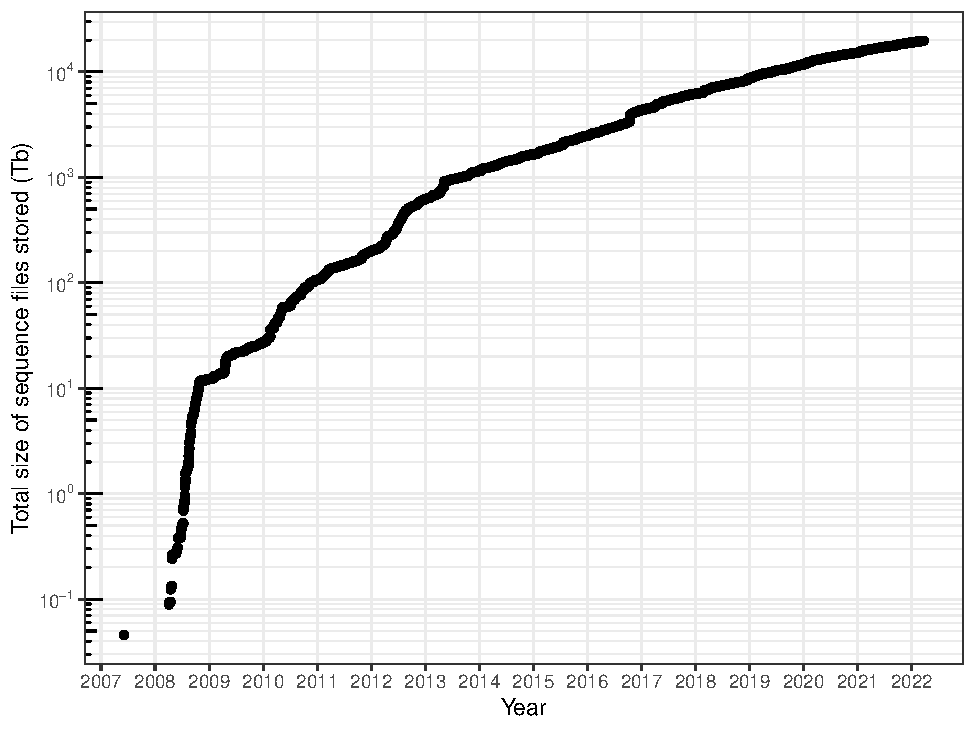
\includegraphics[width=0.8\linewidth]{_main_files/figure-latex/sra-tb-1} \end{center}

\caption{Total size (Tb) of sequence files stored in NCBI's SRA database. \label{fig:sra-tb}}
The SRA database hosts plenty of publicly accessible results of nucleic acid high-throughput sequencing experiments shared by the National Center for Biotechnology Information (NCBI), the European Bioinformatics Institute (EBI) and the DNA Data Bank of Japan (DDBJ). Data retrieved from https://www.ncbi.nlm.nih.gov/sra/docs/sragrowth/ on 23th march 2022.
\end{figure}

Typically, the number of variables \(p\) greatly outnumbers that of observations \(n\) in omics datasets, especially in those of genomics and transcriptomics. This imbalanced high-dimensionality poses several challenges for statistical analysis, such as variable selection, studying interaction effects or the trade-off between false positives and false negatives when testing thousands of hypotheses \autocite{Korthauer2019,Yamada2020}. Also, from a computational viewpoint, storing and processing of omics raw data requires the development of efficient methods, algorithms and pipelines, which has been an important task in the field of bioinformatics \autocite{Berger2013} as the volume of omics data generated kept growing every year (Figure \ref{fig:sra-tb}).

Because of the high amount of information contained within a single omics dataset, it is virtually impossible to consider it exhausted after the analysis by its original authors. The application of different methods on a single omics dataset yields different results \autocite{Yamada2020}. In this sense, it can be assumed that two experimental steps exist: before and after raw data generation, the former \emph{ex silico} and the latter \emph{in silico}. Therefore, public availability and proper metadata annotation of omics data is not only seen as a good practice in terms of reproducibility, but also for reusability \autocite{Perez-Riverol2019}.

\hypertarget{metatranscriptomics-in-the-era-of-rna-seq}{%
\subsection{(Meta)transcriptomics in the era of RNA-Seq}\label{metatranscriptomics-in-the-era-of-rna-seq}}

The development of deep-sequencing technologies, alternatively called next-generation sequencing (NGS) technologies, has effectively widened the range of possibilities within genomics as well as transcriptomics. In the second half of the 2000s, the irruption of RNA-Seq caused a qualitative leap with respect to Sanger sequencing and hybridization-based methods in many aspects. Compared to microarrays, RNA-Seq \emph{(i)} does not rely on previously studied genomes and is therefore suitable for \emph{de novo} approaches on non-model organisms, \emph{(ii)} has a higher sensitivity and a much larger dynamic range of RNA molecule abundance levels and \emph{(iii)} its results are more reproducible, allowing for robust cross-experimental comparisons \autocite{Wang2009}.

To date, second generation sequencing data continues to dominate public repositories of transcriptomic data, although third generation approaches are thought to establish as a standard technology in the near future \autocite{Athanasopoulou2021}. In short, a typical \emph{shotgun} style second generation RNA-seq workflow involves first the isolation of total RNA from a biological sample, followed by an optional step of RNA species (mRNA, rRNA, miRNA, etc.) selection. Then, the remaining population of RNA molecules is subject to fragmentation into shorter sequences of up to 600 bases, due to limitations of second generation sequencing platforms. Afterwards, RNA molecules undergo conversion to cDNA catalyzed by the enzyme reverse transcriptase, and so a cDNA library is constructed. In the process, a series of adapters and barcode identifiers are attached to the ends of the RNA/cDNA fragments by ligation and/or amplification. Each cDNA fragment is sequenced from one end (single-end reads) or both ends (paired-end reads), with a read length of around 100 bp \autocite{Hrdlickova2017}. Once the RNA-Seq read data is formatted in a text file, the bioinformatic procedure begins. Here, a common first goal is to reconstruct the RNA molecules existing in the original sample by aligning overlapping regions between the reads. Finally, the abundance of each RNA molecule can be inferred from the read count assigned to each assembled sequence after a length correction. The detection sensitivity and the accuracy of abundance estimation depend on the read depth, which must be chosen according to the prior knowledge of the biological sample and the aim of the experiment \autocite{Kukurba2015}.

One fundamental problem of second generation sequencing is the assembly of ambiguous reads into `chimeric' contigs\footnote{A contig is a continuous sequence produced by alignment of overlapping reads. Contigs try to reproduce the original molecules from which a particular set of fragments was derived.}, as one single read can be mapped into homologous regions of physically different molecules. The probability of a read being ambiguous decreases as the read length increases. Therefore, the sequencing of full-length cDNA (FL-cDNA) with third generation sequencing platforms is indeed promising, as this technology also accounts for mRNA splicing variants. However, the higher cost per base and the higher base calling error rates continue to hinder its rise as the most popular technology for transcriptome profiling \autocite{Krizanovic2018}.

In many cases, the motivation of transcriptomics studies is to find differentially expressed genes between conditions, focusing on the abundance of nuclear genome-encoded mRNAs. However, many other applications arise considering the diverse origin of RNA molecules that can be found within a biological sample. The prefix \emph{meta-} is added to genomics and transcriptomics when taking into consideration the microbial DNA and RNA content, respectively. Both provide different perspectives for the estimation of the community composition of a microbiome associated to a tissue, organism or simply to an environmental sample, e.g.~soil, freshwater or seawater. While in the 20th century microbiologists approached the study of microbial community and function by isolating and culturing individual species in a reductionist manner, the parallel analysis of the different and potentially unculturable components of a microbial community through metagenomics and metatranscriptomics has revolutionized the understanding of their role in geochemical processes and the biosphere. Apart from that, these new approaches have led to an unprecedented description of microbial phylogenetic diversity \autocite{Mardanov2018}.

The choice of DNA or RNA as the source of information is the fundamental difference between metagenomics and metatranscriptomics and affects the conclusions that can be drawn from the analysis. In metagenomics, usually a phylogenetic marker like 16S rRNA gene is surveyed for classification of individuals into operational taxonomic units (OTUs). This prokaryotic gene is highly-conserved yet polymorphic enough to show differences between species, but also within species in some cases \autocite{Pei2010}. Then, the estimated abundance of each OTU is proportional to the number of 16S rRNA of that particular OTU found within the sample, which serves as an indirect measure of the number of genomes. Although this gene alone could be targeted by PCR\footnote{Polymerase Chain Reaction (PCR) is a method used in molecular biology to replicate the DNA sequence between two known regions in order to obtain a large number of copies of that sequence (amplification). In NGS, fragments are amplified thanks to the adapters that flank them and whose sequence is determined by design.} amplification and amplicon sequencing, the shotgun sequencing alternative is becoming more popular for its sensitivity \autocite{Durazzi2021}, lack of bias \autocite{Brooks2015} and presence of genomic information that can complement 16S rRNA analysis. However, in regards to function, the presence of different genes provides information about potential function, but does not serve as an evidence for effective gene expression.

Meanwhile, metatranscriptomics is more suitable for functional annotation, because RNA molecules are generally the product of transcription and therefore show activity of the genes of a community member. However, it can be argued that mRNA presence alone does not strictly result in gene expression, i.e.~translation into functional protein \autocite{Vogel2012}. While it is also possible to perform taxonomic classification of reads or contigs in metatranscriptomic datasets similarly to metagenomics, the dynamics of RNA molecule population allow for the longitudinal study of the activity of community components over time and in response to changes in the environment \autocite{Shakya2019}.

\hypertarget{virome-profiling-with-metatranscriptomics}{%
\subsection{Virome profiling with metatranscriptomics}\label{virome-profiling-with-metatranscriptomics}}

Alongside microorganisms, DNA and RNA pools of biological samples can also contain molecules of viral origin. Therefore, metagenomics and metatranscriptomics approaches can be directed towards the characterization of viral communities and identification of novel viruses. Again, this method for virome profiling is less biased and more powerful than culture-dependent methods \autocite{Mokili2012}. The lesser-used term `metavirome' is employed in the sense of a sum of viromes to stress the diversity of hosts that viruses have within a particular sample, especially in environmental ones. However, the distinction is rather vague and viruses hosted by different organisms that form part of a symbiosis \autocite{Garcia-Lopez2019} or an ecosystem \autocite{Kim2017} are often referred to as part of the virome.

There are several key differences between microbiome and virome analyses. First, there is no phylogenetic marker similar to 16S rRNA that is applicable to all classes of viruses \autocite{Rohwer2002} (see \ref{quick-overview-on-the-origin-evolution-and-ecology-of-viruses}), although genes encoding the RNA-dependent RNA polymerase (RdRp) and reverse transcriptase (RT) are highly conserved in RNA viruses and reverse-transcribing RNA viruses, respectively \autocite{Koonin2009}. Second, the election of DNA or RNA as a source of information has further implications because of the different types of viral genomes. DNA sequencing can provide information about DNA virus genomes and intermediate forms of reverse-transcribing viruses and proviruses, while metatranscriptomics can survey the whole population of RNA molecules, including transcripts of transcriptionally active DNA and RNA viruses and genomes of RNA viruses.

\emph{Metaviromics} has already reshaped our knowledge on the ecology and evolution of viruses \autocite{Koonin2018}. For example, (a) the diversity, community dynamics and potential role in the carbon cycling of RNA viruses in soil has recently been addressed \autocite{Starr2019}, (b) longitudinal studies have shown the individuality and stability of human gut virome, in line with what was known about gut microbiome \autocite{Shkoporov2019}, (c) the discovery of the ubiquitous presence of RNA viruses in marine environments, where they were thought to be scarce \autocite{Culley2018} and d) metaviromics has allowed for the identification of widespread horizontal gene transfer between viruses of different Baltimore classes and virus transfer between plants, fungi and animals, especially invertebrates, emphasizing the network-shaped nature of RNA virus evolution \autocite{Wolf2018,Dolja2018}.

\hypertarget{state-of-the-art-in-invertebrate-metaviromics}{%
\section{State of the art in invertebrate metaviromics}\label{state-of-the-art-in-invertebrate-metaviromics}}

In regards to invertebrate metaviromics, many recent studies focus on applying the systematic framework of metaviromics to a particular taxon of interest in order to discover novel viruses and describe the diversity of its virome. It is important to note that in most cases, the aggregate of viral sequences identified by deep-sequencing includes viruses that infect different parts of the holobiont with the invertebrate as the host. Furthermore, depending on the sampling conditions, contamination with viruses outside the holobiont can be found, e.g.~viruses of plants, fungi or bacteria. Therefore, it is not a target of metaviromics \emph{per se} to define the host range of the identified viruses, but to identify the presence and abundance of the different assigned viruses. If a found virus shows significant sequence similarity with a known virus, it can be used to deduce its original host.

Anthropocentrically important species draw most of the attention in invertebrate metaviromics. The RNA virome of hematophagous arthropods like ticks \autocite{Meng2019} and biting midges \autocite{Modha2019} has been recently characterized in an effort to evaluate the risk of zoonotic disease emergence in humans or livestock. At the same time, the RNA viromes of vectors of plant diseases like aphids \autocite{Kondo2020} and whiteflies \autocite{Huang2021} have been profiled. Thus identifying the dynamics and effects of different virome compositions on the host phenotype, consequently leading to the proposal on the use of host disease-inducing viruses as biocontrol agents \autocite{Feng2017}. Apart from arthropods, metaviromics have been applied in echinoderms to examine the cause of wasting disease in starfish based on differences in virome composition \autocite{Hewson2020}. Also, the DNA virome associated with the Porifera species \emph{Haliclona fulva}, a sponge holobiont with low microbial abundance, has been recently studied, showing an unexpected low abundance and diversity of bacteriophage families \autocite{Garcia-Bonilla2021}. As for cnidarians, the whole DNA and RNA virome for a sea anemone model species, using publicly available RNA-Seq data, showed a core of viral families found across all samples and how the virome could change depending on the association with a symbiotic alga \autocite{Bruwer2018}. Cnidarians have historically attracted much attention in invertebrate metaviromics, not only because of their ancient divergence during the evolution of metazoans and their richness in symbiotic relationships, but also because of the environmental importance of coral reef ecosystems \autocite{VegaThurber2008}.

The examples of invertebrate metaviromics studies presented above focus on one or a narrow spectrum of related species. Other authors have focused on studying the virome profiles across higher taxonomic ranks, identifying the differences that can occur within and between phyla. In 2019, a study was published surveying the negative single strand RNA virome of more than one thousand insect species using amino acid profile hidden Markov models of the RdRp gene on transcriptomic datasets, thus identifying novel viruses and significant virus-insect co-evolution \autocite{Kafer2019}. As for Porifera, a recent publication revealed that the DNA virome of 15 sponge species is dominated by bacteriophages of the order \emph{Caudovirales} and NCLDVs of eukaryotes , also showing how the virome composition can change depending on the geographical location and nutritional strategy of sponges with PERMANOVA analysis \autocite{Pascelli2020}. A study published in 2021 comparing the viromes of marine Annelida, Arthropoda and Mollusca led to similar conclusions, confirming that the geographical region has an effect on virome composition \autocite{Zhang2021}. In 2016, a comparative analysis of the DNA viromes of four different groups of marine invertebrates (Arthropoda, Cnidaria, Echinodermata and Urochordata) acknowledged the disparities of the viromes within arthropods and the similarities between the viromes of marine arthropods and echinoderms, among other findings \autocite{Gudenkauf2016}.

Fewer studies in metaviromics have tried to assess the diversity of the viromes across a higher number of invertebrate phyla. In 2016, Shi et al.~presented a pioneering work on the global RNA virosphere of invertebrates, sampling metatranscriptomic data of 220 aquatic and terrestrial species of eight invertebrate phyla. They found novel viruses, proposed new viral families, filled major gaps in the RdRp phylogeny and evaluated the degree of virus-host co-divergence and horizontal virus transfer in the history of RNA virus families of invertebrates \autocite{Shi2016}. A related publication in 2019 surveyed the community of transcriptionally active DNA viruses in the same set of species from metatranscriptomic data \autocite{Porter2019}. Both studies show an unprecedented viral diversity in the invertebrate-associated virosphere and stress the difficulty of host assignment to metaviromics-identified viruses and the bulk of viruses that remain unknown. The identification of new viruses is limited and biased by sequence alignment-based taxonomic classification, as the viruses more distantly related to those available in public databases will remain preferentially hidden in high-throughput analyses. Earlier this year, a review was published that discussed the state of the current knowledge on the animal virosphere, proposing the sampling of poorly explored invertebrate phyla and animals of diverse habitats as a priority for the near future in order to better understand animal virome diversity and evolution \autocite{Harvey2022}.

\hypertarget{perspectives-of-the-present-work}{%
\section{Perspectives of the present work}\label{perspectives-of-the-present-work}}

In this study we propose a large-scale application of a metaviromics workflow on more than a thousand transcriptomic datasets of more than 30 invertebrate phyla, all publicly available in the NCBI SRA database \autocite{Leinonen2011}, also including the subphylum of chordates formerly known as Urochordata (now Tunicata). The project will cover organisms belonging to invertebrate phyla with a lack of previous virome analyses such as Kinorhyncha, Placozoa, Priapulida or Tardigrada, just to name a few. Besides, this study will also serve as an example of meta-analysis of transcriptomic data from the SRA database, discussing the state of the available metadata in the context of data reusability.

One of the main goals is to discover the variability of the RNA and DNA virome composition in terms of viral families, within and between as many phyla of invertebrates as possible. Additionally, the effect of the habitat of the host species on the viromes will be evaluated, including terrestrial, marine and freshwater samples, among others. An important point of the study will address the consistency of the results related to species with previously explored viromes in order to validate the bioinformatics pipeline employed.

\hypertarget{materials}{%
\chapter{Materials}\label{materials}}

\hypertarget{data-frame-preparation}{%
\section{Data frame preparation}\label{data-frame-preparation}}

An original data frame was provided by researchers of the biodiversity and evolution of invertebrates Rosa Fernández and Ana Riesgo, affiliated to the Institut de Biologia Evolutiva (UPF-CSIC, Barcelona) and the Museo de Ciencias Naturales (CSIC, Madrid), respectively. This database comprised 8153 unique SRA, BioSample and BioProject identifiers. To contextualize, these three NCBI databases are hierarchically related: a BioProject is a collection of one or more BioSamples and a BioSample contains one or more run accessions in the SRA database, that connects each identifier with its corresponding raw read sequence files in fastq format (one file in the case of single-end reads and two for paired-end reads). Each one of these databases harbors metadata annotated by the original authors of each entry that gives some sort of technical and biological background to the uploaded data.

This collection of invertebrate RNA-Seq datasets was originally used within the frame of an unpublished project of CSIC's LifeHUB.CSIC: Conexión-Vida initiative in evolutionary biology with the aim of resolving and improving the resolution in the tree of life, specifically in the branches related to invertebrates. In this project, the phylogeny of invertebrates of more than 30 phyla was approached by targeted analysis of mitochondrial genes 16S rRNA and cytochrome c oxidase subunit I (COI). As it has been previously introduced, RNA-Seq datasets harbor a large amount of information that can accomodate studies with very diverse goals other than that of their original authors, including analysis of viral sequences.

\begin{table}[!h]

\caption{\label{tab:phyltab}RNA-Seq data sampling depth across the 32 invertebrate phyla included in the final data frame.}
\centering
\resizebox{\linewidth}{!}{
\begin{tabular}[t]{lcclcc}
\toprule
Phylum & Unique species & Run accessions & Phylum & Unique species & Run accessions\\
\midrule
\cellcolor{gray!6}{Annelida (ANN)} & \cellcolor{gray!6}{105} & \cellcolor{gray!6}{497} & \cellcolor{gray!6}{Micrognathozoa (MIC)} & \cellcolor{gray!6}{1} & \cellcolor{gray!6}{1}\\
Arthropoda (ART) & 713 & 1418 & Mollusca (MOL) & 100 & 112\\
\cellcolor{gray!6}{Brachiopoda (BRA)} & \cellcolor{gray!6}{8} & \cellcolor{gray!6}{38} & \cellcolor{gray!6}{Nematoda (NMD)} & \cellcolor{gray!6}{129} & \cellcolor{gray!6}{1936}\\
Bryozoa (BRY) & 9 & 54 & Nematomorpha (NMM) & 3 & 6\\
\cellcolor{gray!6}{Chaetognatha (CHA)} & \cellcolor{gray!6}{10} & \cellcolor{gray!6}{10} & \cellcolor{gray!6}{Nemertea (NME)} & \cellcolor{gray!6}{21} & \cellcolor{gray!6}{69}\\
Cnidaria (CNI) & 231 & 2696 & Onychophora (ONY) & 30 & 58\\
\cellcolor{gray!6}{Ctenophora (CTE)} & \cellcolor{gray!6}{23} & \cellcolor{gray!6}{180} & \cellcolor{gray!6}{Orthonectida (ORT)} & \cellcolor{gray!6}{1} & \cellcolor{gray!6}{2}\\
Cycliophora (CYC) & 3 & 3 & Phoronida (PHO) & 4 & 9\\
\cellcolor{gray!6}{Dicyemida (DIC)} & \cellcolor{gray!6}{2} & \cellcolor{gray!6}{6} & \cellcolor{gray!6}{Placozoa (PLA)} & \cellcolor{gray!6}{4} & \cellcolor{gray!6}{12}\\
Echinodermata (ECH) & 50 & 371 & Platyhelminthes (PLT) & 126 & 23474\\
\cellcolor{gray!6}{Entoprocta (ENT)} & \cellcolor{gray!6}{4} & \cellcolor{gray!6}{4} & \cellcolor{gray!6}{Porifera (POR)} & \cellcolor{gray!6}{44} & \cellcolor{gray!6}{224}\\
Gastotricha (GAS) & 5 & 11 & Priapulida (PRI) & 5 & 6\\
\cellcolor{gray!6}{Gnathostomulida (GNA)} & \cellcolor{gray!6}{2} & \cellcolor{gray!6}{4} & \cellcolor{gray!6}{Rotifera (ROT)} & \cellcolor{gray!6}{16} & \cellcolor{gray!6}{102}\\
Hemichordata (HEM) & 7 & 57 & Tardigrada (TAR) & 7 & 46\\
\cellcolor{gray!6}{Kinorhyncha (KIN)} & \cellcolor{gray!6}{1} & \cellcolor{gray!6}{1} & \cellcolor{gray!6}{Urochordata (URO)} & \cellcolor{gray!6}{9} & \cellcolor{gray!6}{127}\\
Loricifera (LOR) & 1 & 1 & Xenacoelomorpha (XEN) & 17 & 72\\
\midrule
\cellcolor{gray!6}{-} & \cellcolor{gray!6}{-} & \cellcolor{gray!6}{-} & \cellcolor{gray!6}{Total} & \cellcolor{gray!6}{1691} & \cellcolor{gray!6}{31607}\\
\bottomrule
\end{tabular}}
\end{table}

Additional information in the data frame associated with each accession was the habitat and taxonomic information about the invertebrate host species sampled, i.e.~phylum, order, family and the scientific name of the species, amassing 1925 unique species. However, order and family annotation was only complete in Arthropoda, Mollusca and Porifera phyla. Habitat values were missing in 16 phyla, including Nematoda and Platyhelminthes, to name the most represented ones. Habitat annotation was completed by consulting online resources such as the World Register of Marine Species (WoRMS) \autocite{worms} and BioSample metadata when available. This collection of accessions was the result of a collaboration between different researchers specialized in different phyla. Therefore, data frame structure, variable names and values had to be completely standardized before proceeding.

Once done, the objective was to construct a new data frame with as many rows as SRA identifiers (or run accessions) expanding BioSample and BioProject rows into several new ones. An \emph{ad hoc} python script was developed to parse the original data frame by its identifiers to systematically expand them into run accessions and extract metadata from the corresponding NCBI databases using \texttt{esearch}, \texttt{efetch} and \texttt{esummary} functions of \href{https://www.ncbi.nlm.nih.gov/books/NBK179288/}{Entrez Direct}(a command line implementation of Entrez Programming Utilities), combining the retrieved information with that of the original data frame. Metadata was used to confirm and complete the taxonomic assignment of each run accession and to reassure that the sequencing library was indeed generated by RNA-Seq. Apart from that, other columns were constructed based on metadata fields such as file size, isolation source and geographical location. After ignoring accessions corresponding to experiments with DNA and EST libraries that were contained in some BioSamples, the result was a final data frame with 31607 unique run accessions (Table \ref{tab:phyltab}).

Extracted species names coincided mostly with those in the original data frame and the majority of mismatches were due to orthographic inconsistencies, synonymous names and subspecies or laboratory strain overspecification, which were modified to match a name of the species' taxonomic rank. A minority of accessions presenting other types of species mismatching and resulting even in phylum confusions were corrected according to the information present in their corresponding BioSample and SRA entries. Definitive species designation was finally achieved after normalizing names in samples of uncertain species, writing the lowest certain taxonomic rank followed by the ``sp.'' abbreviation, which occurs in 278 species. The whole process of standardization led to an artificial decline in species diversity to 1691 species. The final data frame is available in this project's \href{https://github.com/palf98/metaviromics}{GitHub repository}.

\hypertarget{population-statistical-unit-and-variables}{%
\section{Population, statistical unit and variables}\label{population-statistical-unit-and-variables}}

From a statistical point of view, this project is conceived as an observational study, directed towards descriptive (alternatively associational) inference rather than causal questions. Therefore, the aim is to extrapolate correlations found in the sample between response and covariates to a population scale. The population is defined as the whole possible invertebrate environmental or laboratory samples. It is worthy to note that each individual of this population is referred to as a sample in a biological sense, as it can consist of a body part, an individual or a set of individuals given the size of the organism and the original aim of the authors of each experiment. The subset of these biological samples with publicly accessible transcriptomes comprise the units of observation, i.e.~the level at which the variables are measured. Furthermore, only a fraction of all possible units of observation will be included in the analysis. As the results will be informative not only for the included samples, the unit of analysis ignores the limitation of data availability and is constituted by the individuals of the previously defined population. Thus, the units of observation are contained within the units of analysis.

The availability of data is a source of bias, as the observations are not random draws of the population, but biological samples of interest for a particular group of researchers. Therefore, it is to be expected that the distribution of taxons and habitats in the units of observation differs from that of the units of analysis. For instance, the number of observations of Platyhelminthes samples exceeds by several orders of magnitude that of classically undersampled phyla (Table \ref{tab:phyltab}), but this does not speak about their abundance within the possible invertebrate samples, but the attention they have received by researchers.

For each biological sample, different variables are measured with the aim of studying their effect on virome composition and controlling errors and biases. In the first place, several hierarchically related categorical variables serve as the source of taxonomic information for each observation. For practical reasons and incompleteness of other taxonomic ranks, only the species and phylum factors are included in the analysis. Intermediate ranks can provide an explanation for unexpected results if it has been considered that each species is equally related to the rest of species within a phylum, e.g.~disparate clusters within a phylum. Given the relevance of virus-host co-evolution in invertebrates, we hypothesize that the phylum factor might have an effect on virome composition.

A second categorical variable is comprised by the habitat factor, which divides the biological samples in six categories: terrestrial, marine, freshwater, intertidal zone (littoral zone within the tidal range), brackish water (water of intermediate salinity between freshwater and seawater commonly occuring in estuaries) and saline lakes. The taxonomy of an organism is not independent from its habitat, e.g.~if it is known that an organism belongs to Cnidaria phylum, most certainly it will be a marine species. However, species of other phyla such as Annelida, Arthropoda or Platyhelminthes can live in a variety of habitats. The hypothesis behind the consideration of the habitat factor is that the contamination by other organisms, each carrying its own viruses, differs depending on the habitat, therefore shaping the sample's virome composition. Habitat factor also can account for horizontal virus transfer as it can explain for example the presence of terrestrial plant viruses in terrestrial invertebrates with lifestyles associated with plants.

However, there is a downside to the explaining power of this variable, namely the uncertainty about the sampling conditions of each biological sample. This factor assumes that the natural habitat for each species is equally relevant for all samples, but different researchers could have applied diverse measures to control environmental contamination or even grown the samples in the laboratory. A categorical variable of binary outcome was defined to assign a labstock origin to the samples that were tagged as such under the ``isolation source'' BioSample metadata field, with the hypothesis that the diversity of viral families in these samples is lower than in the rest. This affects 299 accessions of 69 species. Furthermore, the diversity in lifestyles within the different habitat categories is unequal, e.g.~terrestrial habitat includes soil free-living invertebrates, endo- and ectoparasites of animals and plants, while intertidal zone refers to a more specific range of lifestyles. Therefore, the diversity of contamination sources is expected to be larger in less accurately defined habitats.

Geospatial information was also retrieved from BioSample metadata fields ``geographical location'' and ``latitude and longitude'' coordinates. Nevertheless, this information is widely incomplete and hinders the possibility of a spatial analysis at a large scale, as coordinates could only be recovered for less than 500 species representing a lower amount of phyla. Still, this information is valuable to demonstrate the geographical diversity of the samples (Figure \ref{fig:worldmap}).

\begin{figure}[!htbp]

\begin{center}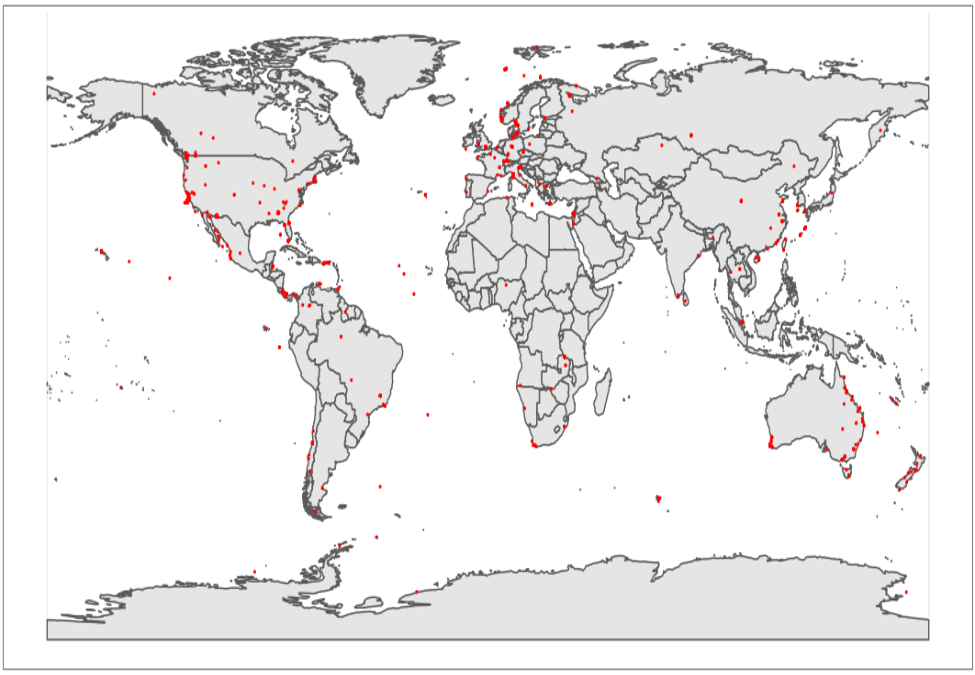
\includegraphics{_main_files/figure-latex/worldmap-1} \end{center}

\caption{Geographical diversity of the biological samples. \label{fig:worldmap}}
Distribution of the 1072 run accessions with available latitude and longitude data. A majority of the points are found near populated areas of North America, Oceania and Europe, while other regions, e.g. Central Asia and Africa, remain underrepresented. Although the spread of locations is unequal, the study can be considered global by the geographical diversity of the observations.
\end{figure}

Another variable that was controlled was the number of bases sequenced in each run accession, which constitutes a quantitative discrete variable. This measure is related to the number of reads, read length and, ultimately, sequencing depth. So, sequencing depth is estimated without having to download sequence files and parsing them character by character afterwards. The values in the available accessions range between 0 and 150 Gbases with an average of approximately \(7.7\) Gbases after sampling one random accession per species. We hypothesize that accessions with lower number of bases will yield a lower virome diversity as lower sequencing depth is associated with a loss of sensitivity.

One can think of many uncontrolled variables that can affect virome composition in this meta-analysis. First, the time of the year and the temperature can affect the community composition of a biological sample, indirectly affecting its virome composition. Furthermore, not only communities are dynamic, but also their transcriptomes are responsive even to different times of the day. As it has been mentioned, the experimental conditions and procedures also can have an effect on virome composition, e.g.~a selection of polyadenylated\footnote{Alternatively poly-A or poly(A). Typically, a 3\(^\prime\) poly-A tail is added in the process of mRNA maturation.} RNA molecules in some samples but not in others would result in a differential representation of RNA viruses, since non-polyadenylated RNA virus genomes will be excluded from the pool of sequenced polyadenylated molecules. Other kinds of experimental procedures such as the sequencing platform and the presence of a viral particle enrichment step previous to sequencing could bias virus identification. In an ideal scenario, these variables could be controlled with proper standardized metadata annotation, which would allow for more ambitious meta-analyses, including spatial and longitudinal studies.

Finally, the virome composition constitutes the multivariate response. After the application of the bioinformatics pipeline, the raw sequences are translated into vectors formed by viral family abundance values for each observation with as many components as viral families identified overall. Depending on the metrics used for abundance estimation, the variables that compose the vector can be discrete (e.g.~number of reads) or continuous (e.g.~transcript abundance per million transcripts). However, relative abundances are always continuous. The characteristics of compositional data will be discussed in the next section.

\hypertarget{pilot-test}{%
\chapter{Pilot test}\label{pilot-test}}

The election of a particular pipeline has an effect on the results obtained and has to be made according to the type of data and the study objectives. In order to compare the results and the scalability of different bioinformatics pipelines prior to the definitive analysis, a reduced subset of 100 accessions was randomly sampled from the original data frame. Since these accessions also contained BioSamples and BioProjects, the number of run accessions was higher, in fact, 138. All programs were tested and run in the HPC cluster `Garnatxa' of I\(^2\)SysBio (UV-CSIC).

\hypertarget{pilot-bioinf}{%
\section{Bioinformatic methods}\label{pilot-bioinf}}

\hypertarget{download-and-pre-processing}{%
\subsection{Download and pre-processing}\label{download-and-pre-processing}}

Three different programs were tested for the download of sequence files and compared in terms of minutes elapsed per GB of compressed sequence file (\texttt{.fastq.gz} format) at \texttt{gzip}'s default compression level: \emph{(i)} fastq-dump, \emph{(ii)} fasterq-dump and \emph{(iii)} parallel-fastq-dump.

Fastq-dump is the standard, basic program to download fastq sequence files from SRA database included in the \href{https://github.com/ncbi/sra-tools}{SRA Toolkit}. Fastq-dump of SRA Toolkit version 2.11.2 was used with \texttt{--split-files} and \texttt{--gzip} arguments to divide forward and reverse reads in paired-end data and to compress the fastq files after downloading, respectively. The result was a rate of 9 minutes elapsed per GB of fastq compressed file.
Fasterq-dump is an alternative program also built in SRA Toolkit which allows parallelization into multiple threads to speed up the download step. As it lacks an option to compress downloaded fastq files, \href{https://leimao.github.io/blog/Parallel-Gzip-Pigz/}{pigz} version 2.3.4, a parallel implementation of \texttt{gzip}, was used down-stream to compress the sequence files downloaded with fasterq-dump.
Finally, the third program tested was \href{https://github.com/rvalieris/parallel-fastq-dump}{parallel-fastq-dump}. Parallel-fastq-dump allows the division of files in blocks that are processed independently by different fastq-dump jobs to concatenate the results in the end. Two methods with parallel-fastq-dump version 0.6.7 were tested, one with the native compression \texttt{--gzip} option included in fastq-dump and the other with pigz compression over the downloaded fastq files.

The method involving fasterq-dump and pigz was reported to be the fastest at roughly one minute elapsed by GB of compressed sequence file. This is a 47\% faster than parallel-fastq-dump with \texttt{--gzip} option, the second fastest method (Table \ref{tab:fqd-speed}). Compressed fastq files were chosen over plain fastq files as the programs in downstream analyses allow processing of compressed fastq files.

Once the download was finished for all selected accessions, Trimmomatic \autocite{Bolger2014} version 0.39 was used over the raw reads to filter technical sequences such as adapters introduced by NGS platforms and low quality reads with base call accuracy equal or greater than 99.95\% (Phred score 33). Trimmomatic was run with 25 threads and did not require any further optimization, as it works fast enough to not represent a limiting step in the pipeline. An accession of approximate average size (7 Gb) was processed by Trimmomatic in approximately 14 min.

\hypertarget{kaiju}{%
\subsection{Taxonomic classification at read level with Kaiju}\label{kaiju}}

Once the sequence files are trimmed and filtered, assembly-free taxonomic classification methods can be applied over the reads. \href{https://github.com/bioinformatics-centre/kaiju}{Kaiju} \autocite{Menzel2016} is a classification program developed for metagenomics and metatranscriptomics datasets that relies on the Burrows-Wheeler transform of protein sequences to speed up the comparison of reads to a reference database. Alignment of amino acid sequences allows to identify more ancient and divergent relationships and is therefore more sensitive than nucleotide-level comparisons in this context.

In short, sequencing reads are translated into the six possible reading frames and split into fragments by the stop codons found. For each read, the taxonomic lineage of the most similar database match to any of its fragments is retrieved and linked to that read. Kaiju uses two methods to estimate the similarity of matches: \emph{(i)} match length for exact matches, i.e.~maximum exact match (MEM) mode, and \emph{(ii)} alignment score for inexact matches based on the BLOSUM62 substitution matrix (Greedy mode).

In this study, Kaiju version 1.8.2 was run in Greedy mode with a default maximum of three mismatches. Greedy mode was chosen over MEM mode for being more sensitive and flexible in relation to the protein sequences available in the reference database. The reference database used was the protein version of the Reference Viral DataBase (RVDB) \autocite{Bigot2020} version 22.0, chosen for being highly curated and suitable for detection of viruses in high-throughput sequencing datasets. Also, its smaller size compared to NCBI RefSeq and nr databases makes the Kaiju analysis require less memory and runtime while focusing on virus detection. To avoid an excess of false positives, a BLOSUM62 score threshold of 65 and an E-value cutoff of \(0.01\) were determined. E-value takes into account database size to estimate the expected number of matches with a particular score occurring by chance. The runtime of the described method for an average run accession was approximately 8 minutes using 25 threads.

Each read classified as viral was assigned to a viral family and the read counts related to each viral family \(j = 1, ..., D\) for each run accession \(i = 1, ..., n\) were added, thus constructing an absolute abundance vector \(x_i\) for each individual, with as many components as viral families found. For each run accession, the sum of this vector equals the total number of reads assigned as viral. These vectors can be combined into an abundance matrix \(X (n \times D) = \begin{bmatrix} x_1 \\ \vdots \\ x_n \end{bmatrix}\) and attached to the other variables in the original data frame. To do this, it is necessary to homogenize the dimensionality of the vectors by adding zero values to viral families not found within each run accession.

\hypertarget{assembly-and-transcript-abundance-estimation}{%
\subsection{Assembly and transcript abundance estimation}\label{assembly-and-transcript-abundance-estimation}}

Two main strategies exist to reconstruct transcriptomes from RNA-Seq data by assembling reads into contigs: \emph{(i)} \emph{de novo} assembly and \emph{(ii)} assembly by mapping to reference genomes. In this study, \emph{de novo} assembly was chosen over reference mapping because it removes bias towards viruses of known genomes. Furthermore, mapping to host genomes to filter host sequences and reduce downstream workload is not possible, as the study includes many non-model invertebrate species without reference genomes available. However, \emph{de novo} assemblers are very computationally demanding and especially memory-intensive. Two programs for \emph{de novo} assembly of reads were used and compared: \emph{(i)} \href{https://github.com/trinityrnaseq/trinityrnaseq}{Trinity} \autocite{Grabherr2011} and \emph{(ii)} \href{https://github.com/ablab/spades}{rnaviralSPAdes} \autocite{Meleshko2021}. Both methods operate similarly, partitioning the sequences into \emph{k-mers} to generate De Bruijn graphs that are analyzed to identify splicing variants.

Trinity is one of the most sensitive \emph{de novo} assemblers for RNA-Seq data as it aims is to extract as much information as possible. While it assembles a lower number of unique transcripts than other short read assemblers, Trinity does not require as much memory \autocite{Sze2017}. Trinity version 2.13.2 was run in Singularity with default parameters, i.e.~a \emph{k-mer} length of 25 bases, over the trimmed sequencing read files. With 25 threads and a maximum memory usage of 100 GB, Trinity took three hours to process an average-sized run accession.

Alternatively, directed assembly of RNA virus contigs was conducted with rnaviralSPAdes version 3.15.4. This software assembles RNA viruses at species level, collapsing sequences of quasispecies that will certainly coexist in the samples given the high rate of variation of RNA virus genomes. In terms of runtime, assembling with rnaviralSPAdes has been superior to Trinity's, since only 14 minutes were needed for an accession of 7 Gb running with 16 threads. However, this program was discarded for its results in the downstream analyses, since most of contigs assembled by rnaviralSPAdes were not classified as viral, resulting in a low proportion of viral contigs from an overall much lower number of assembled contigs (roughly assembling only 0.16\% of contigs with rnaviralSPAdes compared to those obtained with Trinity).

Once the assembly was finished, the abundance of the RNA molecules in the samples represented by each contig was quantified. For convenience, we will refer to those RNA molecules as transcripts. For that purpose, two programs that are included within Trinity 2.13.2 toolkit were tested and compared: \emph{(i)} \href{https://github.com/deweylab/RSEM}{RSEM} \autocite{Li2011} and \emph{(ii)} \href{https://github.com/pachterlab/kallisto}{Kallisto} \autocite{Bray2016}. RSEM is an alignment-based method that involves mapping the reads to the assembled contigs in order to obtain read count measures to estimate transcript abundance. Meanwhile, Kallisto uses a faster, alignment-free strategy that involves the decomposition of read and contig sequences into \emph{k-mers} to indirectly map the reads to the contigs with a \emph{k-mer} hash table. This approximation has shown to be nearly as accurate as alignment-based methods with real data \autocite{Sarantopoulou2021}. In this study, Kallisto was chosen over RSEM not only for being nearly 39 times faster, but also because RSEM was unstable with our data, failing to give a complete output for \(\sim 11 \%\) of sampled accessions. Kallisto gives an estimation of read counts per transcript and normalized measures for transcript abundance such as TPM (Transcripts Per Million), which accounts for transcript length and sequencing depth to give a corrected measure of transcript relative abundance within the whole transcript population of the sample. This metric takes the sum of reads mapped to contigs as a whole, leaving the unmapped reads out of the equation.

The E90N50 statistic for contigs was computed to assess the quality of the Trinity assembled transcriptomes. This is a modification of the conventional contig N50 traditionally used in genomics, which determines the contig size over which half of the assembled bases are covered in the assembly. In transcriptomics, the addition of the Ex metric is recommended to filter out the least expressed genes and keep the genes that account for the \(x\%\) of the normalized expression. Lowly expressed genes can heavily distort the conventional N50 statistic, since their contigs will tend to be shorter due to their lower coverage. E90N50 was computed with the `contig\_ExN50\_statistic.pl' utility provided in Trinity toolkit using the transcript abundance data estimated with Kallisto.

\hypertarget{taxonomic-classification-at-contig-level}{%
\subsection{Taxonomic classification at contig level}\label{taxonomic-classification-at-contig-level}}

Five different methods were compared in the context of taxonomic classification of contigs in terms of runtime and analysis results in order to choose the best suited method for final analysis of data: \emph{(i)} \href{https://github.com/bbuchfink/diamond}{DIAMOND} \autocite{Buchfink2021}, \emph{(ii)} DIAMOND over \href{https://github.com/jessieren/VirFinder}{VirFinder}'s \autocite{Ren2017} subset of putative viral contigs, \emph{(iii)} DIAMOND over \href{https://github.com/jiarong/VirSorter2}{VirSorter2}'s \autocite{Guo2021} subset of putative viral contigs, \emph{(iv)} \href{https://github.com/dutilh/CAT}{CAT} \autocite{VonMeijenfeldt2019}, and \emph{(v)} \href{https://github.com/hyattpd/Prodigal}{Prodigal} \autocite{Hyatt2010}, \href{http://hmmer.org/}{HMMER} and CAT.

First by order of mention, DIAMOND implements a protein alignment method optimized for massive query datasets and reference databases. The scope of DIAMOND is to perform sequence similarity searches that are similar in sensitivity to BLAST, but at a substantially faster rate. DIAMOND v2.0.13 was used in blastx mode to translate the nucleotide contigs into proteins and to perform alignments against a reference database, in this case, the whole NCBI nr database (downloaded on 15 December 2021). Using the second most sensitive mode of DIAMOND (\texttt{--very-sensitive}), the search and alignment process took roughly \(32\) hours for an average-sized accession, with this step causing a major time increase in the pipeline. DIAMOND's output contains the NCBI taxonomy identifier (TaxID) and the E-value of each hit for each contig. \href{https://bioinf.shenwei.me/taxonkit/}{Taxonkit} \autocite{Shen2021} was used to obtain the family of each hit from its TaxID's. A contig was considered viral when it had a hit taxonomically annotated as viral with an E-value lower than \(1e-05\). Then, the abundance estimation (TPM) for contigs belonging to each viral family were added and the viral families abundance matrix was constructed.

VirFinder and VirSorter2 are two methods that use different strategies to predict \emph{viralness} of contigs and which can be used prior to DIAMOND to reduce its workload at query level. Over the resulting subsets of putative viral contigs, the whole DIAMOND process described above is performed in order to obtain the taxonomic information and construct the abundance matrices. In this context of \emph{viralness} prediction, the balance between false positives and false negatives can be seen as a trade-off between runtime and sensitivity. Thus, a subset of contigs with an excess of false positives, i.e.~host sequences, will make the DIAMOND process take longer. Meanwhile, a subset leaving out a high number of true viral sequences will artificially reduce the viral diversity while speeding up the DIAMOND process.

VirFinder is an R-built method that uses \emph{k-mer} frequency-based Lasso logistic regression models trained on host and virus sequences in order to classify contigs. Different models are fitted for sequences of different lengths, with a reported optimum at lengths of \(1\) to \(3\)kb \autocite{Ren2017}. VirFinder is a binary classifier where the null hypothesis, i.e.~that of a contig not being viral, is tested for each contig. Under this multiple comparisons context, \(p\)-values were corrected by the Benjamini-Hochberg procedure in order to control the false discovery rate (FDR) with \(\alpha = 0.05\). After parallelization, VirFinder version 1.1 runs at a rate of \(4\) min/Gb using the `VF.modEPV\_k8' model, which is trained with prokaryotic and eukaryotic host and virus sequences (script available in \href{https://github.com/palf98/metaviromics}{(https://github.com/palf98/metaviromics)}).

VirSorter2 applies a machine learning-based approach to predict the \emph{viralness} of contigs using different variables including structural, functional and taxonomic features, such as GC content, gene density, gene overlapping frequency or strand switching frequency. Since these variables are highly heterogeneous among major groups of viruses, different models are applied to detect RNA viruses, ssDNA viruses, dsDNA viruses and giant DNA viruses. However, in our case this is only useful not to introduce a bias in the binary virus-host classification towards a particular group of viruses, as a more comprehensive taxonomic classification is then performed by DIAMOND. Each virus group classifier provides each contig with a score in the range of \(0\) to \(1\), where \(1\) means a higher virus call confidence. In this case, a moderate score cutoff of \(0.5\) was used to avoid an excess of false negatives before classification with DIAMOND, which will presumably further reduce the number of viral contigs. VirSorter version 2.2.3 was run in parallel with \(20\) threads, classifiers for RNA, ssDNA and dsDNA viruses and the \texttt{--keep-original-seq} parameter, yielding a processing rate of \(58\) min/Gb.

A fourth method considered CAT as an alternative for taxonomic classification of contigs. Although CAT is originally thought for metagenomic data, the fact that it is more robust compared to DIAMOND and Kaiju in detection of novel viruses made CAT an interesting candidate tool. CAT is a pipeline that involves: \emph{(i)} a prediction of ORFs\footnote{An Open Reading Frame (ORF) is the sequence enclosed between a start codon and a stop codon in the exome or the transcriptome. These two features define the peptide that can be potentially expressed from this ORF after translation of mRNA. The finding of an ORF does not exclude the presence of another valid reading frame in the same region.} and their translation into proteins with Prodigal, \emph{(ii)} similarity searches of the translated protein sequences with DIAMOND in blastp mode against the nr database, and \emph{(iii)} taxonomic classification based on CAT's algorithm. The ORF prediction and translation approach highly reduces the workload for the subsequent DIAMOND step compared to the above described DIAMOND blastx strategy, where contigs are completely translated into proteins in all six reading frames. Once DIAMOND has ended searching for hits, CAT's algorithm gives a last common ancestor consensus between the taxonomic affiliations of the top-scoring hits (E-value \(< 0.001\)) to the protein sequence(s) of a contig. Thus, CAT avoids being overly-specific and can provide a higher taxonomic rank when no clear classification can be done at species level, making it more robust and sensitive to sequences without close relatives in the database. With CAT version 5.2.3, the whole CAT pipeline was run in 1 hour and 18 minutes parallelized with 20 threads for the 7 Gb accession used as benchmark.

The last method uses another strategy to purge non-viral contigs prior to more accurate contig classification by performing a search against profile hidden Markov models (HMMs) of RdRp. First of all, profile HMMs are probabilistic models that gather position-specific information about a set of aligned sequences \autocite{Eddy1998}. This means that the model adapts to the substitutions, insertions and deletions that are found in the multiple sequence alignment and each variation is given a score that depends on the occurrence of those changes in each particular position. In contrast to previous methods, virus detection here is directed only towards RNA viruses, since the high degree of conservation in the aminoacid sequence of RdRp makes the application of profile HMMs advantageous. RdRp profile HMMs were made using \texttt{hmmbuild} function of HMMER version 3.3.2 over nine reference RdRp protein alignments recovered from \href{https://pfam.xfam.org/}{Pfam} (PF00680, PF00972, PF00978, PF00998, PF02123, PF04197, PF05919, PF20483, PF20488). In this step, the underlying probabilistic model that maximizes likelihood to generate the observed sequences in the seed alignment is obtained.

Prodigal version 2.6.3 was used for the purpose of prediction of ORFs in the assembled contigs and their subsequent translation into aminoacid sequences. Once the sequences of the putatively existing proteins are translated, their homology to the different RdRp profile HMMs was examined using \texttt{hmmsearch} function of HMMER. What is being evaluated here is, namely, the compatibility between the hidden model that generated each translated protein sequence and the profile HMMs one by one. Similarly to other sequence similarity search algorithms, each query sequence is given a score and an E-value of which a threshold of \(1e-05\) was used. As these profiles are built with viruses of different families, this is not sufficient classification for our goal, since we are interested in a classification of contigs to specific viral families. Therefore, CAT was used over the significant hits in \texttt{hmmsearch}'s output following the above described method. In terms of computational time requirements, this fifth method is by far the fastest one: for our benchmarking accession, Prodigal was done in approximately 8 minutes and \texttt{hmmsearch} in a few seconds. CAT was very fast because of the few sequences with significant homology to RdRp in \texttt{hmmsearch} analysis. However, less diversity is expected in the viromes obtained with this method due to the loss of DNA viruses by only focusing on RNA viruses via RdRp homology.

In the end, the taxonomic assignments of assembled contigs for all five tested pipelines were processed to match the abundance matrix structure of samples by viral families introduced in \ref{kaiju}. Nonetheless, in the context of contigs, transcript abundances are estimated with TPM units, which are a concentration measure relative to the whole surveyed transcript population. Thus, the sum of each row divided by one million equals the estimated proportion of viral RNA. This is equivalent to the quotient between the assigned viral reads and the total number of reads in the case of reads.

\hypertarget{pilot-stat}{%
\section{Statistical methods}\label{pilot-stat}}

In the previous section, the data structure of the response variable has been shortly introduced in the context of the different pipelines' output. Next, the appropriateness of a compositional approach to the analysis of the obtained viral families abundance tables is discussed. Once the type of data that is being dealt with is defined, some applicable statistical analyses will be presented.

\hypertarget{treatment-of-virome-data-as-compositional-data}{%
\subsection{Treatment of virome data as compositional data}\label{treatment-of-virome-data-as-compositional-data}}

First, it is convenient to recall the aim of this study, which is to identify differences in virome community composition between different groups. More specifically, this purpose is fulfilled by answering questions such as: is viral family A more abundant in sample 1 than in sample 2? To answer this question, it is fundamental to understand that the meaning of abundance in this context is namely the dominance of transcripts of family A with respect to the whole viral transcript population. The values in the estimated abundance tables do not answer this question directly. In the case of read count tables, the values depend on the total number of reads of each experiment, which is variable among the samples. Therefore, the absolute difference for read counts of family A between samples 1 and 2 is not very suitable for virome analysis. This is also the case for TPM tables, where the observed values for every family depend on the sum of viral TPM, which differs between samples, too. Nevertheless, both matrices carry relative information that can be useful to answer such questions. The read counts or transcript concentrations assigned to each viral family represent its contribution to the total viral abundance or the whole transcriptome expression if its non-viral part is also considered. In short, the primary interest lies in the distribution of the identified viral RNA across the different viral families.

The purpose of compositional data is to characterize the parts of some whole \autocite{Pawlowsky-Glahn2015a}. A particular dataset composed of multivariate observations of proportions, concentrations or absolute frequencies can be considered compositional data if the goal is to quantify the relative contribution of each or some of its parts to the total. The source of such relative information is contained implicitly in the data, namely in the ratios between the parts, whose observed values are strictly positive by definition. However, when the absolute amounts and differences constitute the matter of interest, a standard multivariate approach is more appropriate. For these ambivalent multivariate datasets, the distinction between treatments is dependent on the analyst's goals. It is worthy to note that when both the relative information and the total amount are relevant, the latter can be kept and analyzed as a variable external to the compositional structure \autocite{Pawlowsky-Glahn2015b}.

Formally, this treatment distinction draws on the assumption of different underlying sample spaces for the data. In the case of standard multivariate analysis, operations take place in the real Euclidean space. Meanwhile, the sample space for compositional data is the simplex, which is subject to the properties of the Aitchison geometry, i.e.~the algebraic-geometric structure of the simplicial vector space \autocite{Aitchison1982}. The application of common statistical analyses based on Euclidean geometry in the analysis of proportions can lead to incoherent and inconsistent results. This was noted by Karl Pearson in 1897, as he observed that the ratios between uncorrelated random variables showed in fact a \emph{spurious} correlation \autocite{Pearson1897}.

A composition is a vector of strictly positive values with as many elements as parts. Considering a set of \(D\) parts or components, the composition \(x = (x_1, x_2, \ldots, x_D)^\prime\) exists in the positive real D-dimensional space \(\mathbb{R}^D_+\). Compositional data are characterized by the principle of \emph{scale invariance}, which states that the multiplication of a composition by an arbitrary positive scalar does not affect the ratios between components. Therefore, the relative information of compositions is preserved after rescaling to proportions or percentages or after changing units. The \emph{closure operator} \(C\) is used to rescale compositions to have a sum equal to a desired positive constant \(\kappa\) \eqref{eq:closure}. The closure of the previously proposed \(x\) composition to \(\kappa\) stands as

\begin{equation} 
  C_{\kappa}(x) = \left( \frac{\kappa \cdot x_1}{\sum^{D}_{i=1}x_i}, \ldots, \frac{\kappa \cdot x_D}{\sum^{D}_{i=1}x_i} \right).
  \label{eq:closure}
\end{equation}

The property of scale invariance results in the more recent definition of compositions as equivalence classes \autocite{Barcelo-Vidal2016}, where two compositions \(x\) and \(y\) are compositionally equivalent if \(C_{\kappa}(x) = C_{\kappa}(y)\). Or alternatively if \(x\) and \(y\) are proportional, i.e.~if there exists a positive scalar \(c\), such that \(x = c \cdot y\). In this case, \(x\) and \(y\) are just two out of all possible representatives of their equivalence class. A practical approach in the analysis of compositional data is to obtain vectors of proportions by normalizing the compositions to have a constant sum of one. Compositional vectors of D dimensions that sum up to one are easy to represent in the \((D-1)\)-standard simplex \(S^D\), a subset of \(\mathbb{R}^D_+\) whose vertices are formed by all D possible unit vectors of D dimensions:

\begin{equation} 
  S^D = \left\{ x = (x_1, \ldots, x_D)^\prime \in \mathbb{R}^D \mid x_i > 0, \sum^{D}_{i=1} x_i = 1 \right\}.
  \label{eq:simplex}
\end{equation}

However, the principle of scale invariance demonstrates that the constant sum constraint \(\kappa\) is irrelevant in terms of relative information and the sample space of compositions can be generalized for each of its representatives \autocite{Filzmoser2018a}:

\begin{equation} 
  \tilde{S^D} = \bigg\{ x = (x_1, \ldots, x_D)^\prime \in \mathbb{R}^D_+ \mid x_i > 0, \forall \kappa > 0 \, \exists ! c > 0: x = cC_\kappa(x) \bigg\}.
  \label{eq:samplespace}
\end{equation}

Thus, the traditional sum constraint property of compositional data \autocite{Chayes1960} is nowadays disregarded as just a way to obtain a specific representative of a composition's equivalence class \autocite{Egozcue2019}.

Another main principle of compositional data is that of \emph{subcompositional coherence}, which states that the information carried by a composition and any of its subcompositions, i.e.~subvectors, should not contradict. More specifically, this is reflected by the following two properties: \emph{(i)} the distance between two compositions \(x\) and \(y\) is always equal or greater than the distance between two of their subcompositions \(x_s\) and \(y_s\) (\emph{subcompositional dominance}) and \emph{(ii)} the ratios between two parts do not depend on the arbitrary inclusion/exclusion of further parts in the composition or subcomposition (\emph{preservation of ratios}). Although it is also to be expected in other types of multivariate data, \emph{permutation invariance} is the third principle of compositional data. It enunciates that the the order in which the parts of a composition are expressed should not have an effect on the results of the analysis \autocite{Pawlowsky-Glahn2015c,Filzmoser2018b}.

Although ratios are the essential source of information of compositional data, the main approaches to analyze this type of data rely on a specific family of transformations thereof. For instance, consider all pairwise ratios in a composition to a reference part \(\frac{x_i}{x_D}, i = 1, \ldots, D - 1\). The distribution of these ratios is asymmetric in \((0, +\infty)\) with a balance between the weight of both the parts in the numerator and the denominator in 1. The logarithm transformation of the ratios (\emph{logratios}) moves the range to the real line \((-\infty, +\infty)\) and centers the balance in \(0\). Thus, logratios enhance the interpretation of relative information and its mathematical handling.

The logratio methodology was first introduced by John Aitchison \autocite{Aitchison1982} with what is known today as the \emph{move-from-the-simplex} approach. The idea was to find a one-to-one transformation which made it possible to leave behind the simplicial sample space and study compositional data in an unrestricted real space, where common multivariate statistical methods can be applied. Here, logratios can be assumed to follow a Normal distribution, avoiding the geometrical peculiarities of the simplex. Later, the Aitchison geometry of the simplex was described with new basic operators for vector shifting and multiplication by a scalar. This led to redefinitions of norm, inner product and distance for the simplex essentially based on the use of logratios to obtain a Euclidean linear vector space. Once the simplicial sample space was defined as a proper metric vector space, the \emph{staying-in-the-simplex} methodology was born. In this case, compositions are represented by orthonormal logratio coordinates with respect to a generating system, i.e.~the simplex. While both strategies effectively avoid the development of adapted statistical methods to analyze raw compositions directly in the Aitchison geometry and their results are equivalent in some cases, there is a conceptual and rather subtle difference: in the first approach we assume that a log-normal random vector exists in \(\mathbb{R}\) derived from the random composition, while in the second one, the random composition exists in \(\mathbb{R_+}\) and its logratio coordinates are just a representation thereof \autocite{Mateu-Figueras2011}.

The use of (log)ratios makes the presence of zero values in the compositions especially problematic in the analysis of compositional data. Although zero values are excluded from the formal definition of \(\tilde{S^D}\), there are different reasons why zero values can occur in real data. When a continuous variable such as a concentration is being measured, \emph{rounded zeros} can appear in the process of data generation when a recorded value is lower than a certain significance threshold or detection limit. In the case of count data, \emph{sampling zeros} can occur when there is an insufficient sampling depth: although the element is present in the population, it is not sampled and hence, a zero value is recorded. Both presented types of zeros constitute cases similar to not missing at random (NMAR) values, i.e.~the element was present but not detected due to its low abundance. Here, imputation of small values is the way to go \autocite{Martin-Fernandez2011}. \emph{Structural zeros}, also called true or essential zeros, are the result of the absolute absence of a particular component in a population. Therefore, the recorded zero value is not the consequence of a limited sample size or the measuring instruments used and can be understood as a true negative. In this case, there is an essential difference between observations with and without zeros that separates them in different populations \autocite{Pawlowsky-Glahn2015c}. Thus, it seems that the replacement of such zeros, that are informative by themselves, by small values is not adequate.

Fundamentally, viral families abundance tables are not different from other taxa count or percentage matrices used in ecology. The application of compositional data analysis to high-dimensional ecological community compositions is relatively established in the field of microbiome analysis \autocite{Xia2018,Tsilimigras2016}. However, in virome composition analyses, compositional approaches with the use of logratios for exploratory analyses have just recently been introduced \autocite{Zuo2020,Yan2021}. Just as microbiome data, virome data is generated through a process of sequencing and classifying the obtained reads into categories of interest, e.g.~within a taxonomic rank of choice. As to why microbiome and virome data can be treated as compositional, it can be argued that the total sum of reads is not of interest \emph{per se}, since it is an artifact of the experimental procedure, i.e.~the total number of reads or library size. Accordingly, the absolute differences between components do not pose a valuable source of information to describe the contribution of each of the parts to the whole. Also, the observed values in microbiome or virome compositions are always non-negative regardless if they are discrete or continuous.

However, omics-generated compositional data have a series of particular characteristics that can hinder the application of standard statistical approaches. Typically, these studies usually include a small number of observations \(n\) due to their high generation cost and consider the classification of their reads into a larger number of categories \(p\), thus leading to an underdetermined system. In the context of taxonomic classification, the number of possible categories varies drastically depending on the taxonomic rank of choice. For instance, the International Congress for Taxonomy of Viruses (ICTV) recognizes to date (\href{https://talk.ictvonline.org/taxonomy/vmr/m/vmr-file-repository/13426}{Virus Metadata Repository number 19, April 25, 2022; MSL37}) 10434 viral species arranged in 2607 genera, 234 families, 66 orders and so on moving upwards in the taxonomic hierarchy. The number of possible categories also has an effect on another acknowledged feature of virome data, which is a high frequency of zeros in the count matrices (sparsity). The use of OTUs and low taxonomic ranks, which is common in these fields, tends to aggravate both the large \(p\), small \(n\) and the sparsity problems \autocite{Xia2017}. In the present case, the family rank was considered the taxonomic classification criterion for being a balanced source of information, neither too general nor too specific. Besides, the underdetermination problem can eventually be solved with an extensive enough analysis, as the number of analyzed observations surpasses that of observed categories. Also the sparsity problem is alleviated by this decision, although a dominant presence of zeros is still to be expected. Moreover, methods for variable selection and/or dimensionality reduction are common in the context of microbiome and virome data analysis.

Virome taxa tables have notably diverse sources of zero values, which are forced to occur when compositional vectors with different parts are arranged into a matrix. However, it can be especially challenging to distinguish structural zeros from sampling and rounded zeros due to the complex experimental and bioinformatic process used to generate virome data. Structural zeros occur when the sample has an absolute lack of transcripts belonging to a particular viral family. Sampling zeros can be associated with an insufficient library size, low quality reads that are discarded by the trimming step and poor coverage of the family in the reference database used for classification of reads or contigs. To a lesser extent, rounded zeros can appear in the processing of data when converting the count data to relative abundances or other continuous metrics.

As a final remark regarding the features of virome datasets, while observations can be expected to be independent with a proper sampling procedure, the abundance of the different families will not be independent both from a compositional and an ecological point of view. There is a complex correlation structure where the former has an influence in the sense of sum of the parts to a whole (e.g.~consider a composition \(x\), so that \(P( x_{(i=2,\ldots,D)} > 0.8 |\sum_i^Dx_i = 1, x_1 = 0.2) = 0\))) and the latter introduces relationships between virus groups due to phylogenetic and ecological resemblances (e.g.~in a sample where a family of bacteriophages is found, it is likely to find further families of viruses infecting bacteria).

\hypertarget{ecological-diversity-metrics}{%
\subsection{Ecological diversity metrics}\label{ecological-diversity-metrics}}

The observed abundance values for viral families arranged in each compositional vector can also be used to estimate different diversity measures to characterize the virome of a particular biological sample in a non-family-specific manner. First, the simplest considered diversity metric was \(\alpha\)-diversity at family level \(F\). It summarizes the number of different viral families that are found in an observation. This measure of viral families richness can be defined for each observation in the \(X (n \times D)\) abundance matrix as

\begin{equation} 
  F_i = \sum^D_{j=1} f(X_{ij}) \text{, where } f(X_{ij}) = \begin{cases} 1 \text{ if } X_{ij} > 0 \\ 0 \text{ otherwise} \end{cases}\text{,}
  \label{eq:richness}
\end{equation}

\begin{equation*} 
 i = 1,2, \ldots, n \text{ and } j=1,2,\ldots,D\text{.}
\end{equation*}

In second place, the Shannon diversity index \(H^\prime\) was estimated. Unlike richness estimate \(F\), this index takes into account the proportions in which each of the viral families are found. Hence, a community with three families and a vector of relative abundances \(x_A = (\frac{1}{20}, \frac{1}{20}, \frac{9}{10})\) is thought to have a lower entropy than a community with three families with balanced proportions \(x_B = (\frac{1}{3}, \frac{1}{3}, \frac{1}{3})\), where the prediction of a next draw from the population is more uncertain. A high Shannon diversity index indicates that the community harbors a larger diversity. \(H^\prime\) is maximized with increased values of families richness \(F\) and the more balanced the abundances of the families are \autocite{Ludwig1988}. Zero values are ignored for its definition and the total number of parts is reduced to the subset of parts effectively observed for each observation \(F_i\). Abundances are converted to proportions in order to normalize the differences in the sample sizes of different observations. So,

\begin{equation} 
  H^\prime_i =  
  -\sum^{F_i}_{j=1}\left(\frac{x_{ij}}{\sum^{F_i}_{j=1}} \cdot log(\frac{x_{ij}}{\sum^{F_i}_{j=1}}) \right) = 
  -\sum^{F_i}_{j=1}\left(p_j \cdot log(p_j) \right)\text{,}\\
  \label{eq:Shannon}
\end{equation}

where \(F_i \in \{1,2,\ldots,D\} \text{, } i = 1,2,\ldots,n \text{ and } j = 1,2,\ldots,F_i\text{.}\) Note that this operation is not applied to a matrix, but to a collection of vectors of possibly different length.

The balance between viral family proportions for an observation, i.e.~families evenness, can be estimated from the ratio between the obtained \(H^\prime_i\) and its maximum possible Shannon diversity index value \(H^\prime_{i \text{ } max}\), which occurs when the abundances of all families in the community are equally distributed \autocite{Ludwig1988}. \(H^\prime_{max}\) is solely dependent on the number of families \(F_i\), as can be seen in \eqref{eq:Shannon}. Values near to 1 are indicative of a more even distribution of the community components. For every observation, the definition of families evenness index \(E\) from \(H^\prime\) estimate stands as

\begin{equation} 
  E_i = \frac{H^\prime_i}{H^\prime_{i\text{ }max}} = \frac{H^\prime_i}{log(F_i)} \text{, } i = 1,2, \ldots, n.
  \label{eq:evenness}
\end{equation}

It is important to note that the presented diversity measures do not take into account the taxonomic relationship between families and therefore do not provide an estimate for distinctness. For instance, the diversity estimated for a community formed by two viral families will be the same regardless if both families are contained within the same order or if they diverged at higher taxonomic ranks.

\hypertarget{permanova}{%
\subsection{PERMANOVA}\label{permanova}}

Permutational multivariate analysis of variance (PERMANOVA) was performed in order to test if the phylum and habitat factors have an effect on the samples' virome compositions given a dissimilarity measure of choice. In contrast to classical multivariate ANOVA (MANOVA), PERMANOVA is a non-parametric alternative that does not assume any distribution for the data and is relatively robust to heterogeneity of within-group variances and unbalanced designs. Furthermore, PERMANOVA can be applied to high-dimensional data with zero-inflated, overdispersed and underdetermined behavior. For its broad applicability spectrum, PERMANOVA is widely used in ecology to detect alterations in community structure in response to different conditions \autocite{Anderson2017}.

In microbiome and virome community analyses, Bray-Curtis distance is the standard dissimilarity measure used in the context of PERMANOVA, as can be seen in recent examples \autocite{Lu2021,Hegarty2022,Kaelin2022}. Bray-Curtis distance \(BC\) is a standardized version of the Manhattan distance that quantifies the pairwise compositional dissimilarity between two samples based on the discrete or continuous abundance values of their community components. An interesting feature of \(BC\) is that parts absent in both samples are ignored and rare parts have little effect compared to more dominant components. So,

\begin{equation} 
  BC_{ij} = \frac{\sum^D_{k = 1} \left|X_{ik} - X_{jk}\right|} {\sum^D_{k=1}\left(X_{ik}+X_{jk}\right)} \text{ ,}\\
  \label{eq:BrayCurtis}
\end{equation}

where \(D\) is the total number of families found for all samples, \(X\) is the raw \(n \times D\) abundance matrix and \(i,j = 1, ..., n\) with \(n\) being the total number of observations sampled. This operation results in a \(n\times n\) distance matrix with values in the range between 0 and 1, where 0 is indicative of exact resemblance and 1 of complete dissimilarity.

Formally, PERMANOVA is a geometric partitioning of variation across the data in the space of the chosen distance metric in response to one or more factors \autocite{Anderson2017}. When Euclidean distances are used, the null hypothesis (\(H_0\)) states that the positions of the centroids for every group in the dissimilarity matrix are equivalent \autocite{Anderson2013}. However, the term \emph{central locations} is more appropriate for other distance matrices, such as \(BC\). This hypothesis testing requires the estimation of ANOVA-like statistics and finally the obtention of a \(p\)-value through a process of permutation, i.e.~the random shuffling of observations between groups \autocite{Anderson2001}. \(H_0\) operates under the assumption that observations are exchangeable between groups and therefore permutation should not have an effect on the central location of the different groups.

Briefly, the classic ANOVA relationship between the total sum of squares (\(SS_T\)), the within-group or residual sum of squares (\(SS_W\)) and the sum of squares between groups (\(SS_B\)) holds: \(SS_T = SS_W + SS_B\). The PERMANOVA table can be constructed from the following operations:

\begin{equation} 
  SS_T = \frac{1}{N} \sum^{N-1}_{i=1}\sum_{j = i + 1}^N BC^2_{ij}\text{ ,}\\
  \label{eq:SST}
\end{equation}

where \(N\) stands for the total number of observations, \(i = 1,\ldots,N\) and \(j = 2, \ldots, N\);

\begin{equation} 
  SS_W = \sum^G_{g=1}\left(\frac{1}{n_g} \sum^{N-1}_{i=1}\sum_{j = i + 1}^N BC^2_{ij}\varepsilon^{[g]}_{ij}\right),\\
  \label{eq:SSW}
\end{equation}
where \(G\) stands for the total number of groups, \(n_g\) is the number of observations belonging to group \(g\) and \(\varepsilon^{[g]}_{ij}\) is a binary indicator that takes the value 1 when \(i\) and \(j\) belong to group \(g\) and 0 otherwise;

\begin{equation} 
  SS_B = SS_T - SS_W \text{ .}\\
  \label{eq:SSB}
\end{equation}

Now, a ratio between signal (\(SS_B\)) and noise (\(SS_W\)) can be obtained in the form of a pseudo \(F\) statistic:

\begin{equation} 
  F = \frac{\frac{SS_B}{(G-1)}}{\frac{SS_W}{(N-G)}} \text{ .}\\
  \label{eq:pseudo-F}
\end{equation}

Under \(H_0\), this ratio will be near to 1, but when the central locations of the groups really differ, \(SS_B\) will take relatively large values compared to \(SS_W\). This causes an increase in the pseudo \(F\)-ratio. However, since the dependent variables, i.e.~the parts, are neither normally distributed nor independent, a \(p\)-value cannot be obtained the regular way. The permutation algorithm is used to generate an empirical \(F\) distribution from an arbitrary number of re-orderings of the observations (\(M\)). Thus, an alternative for the obtention of \(p\)-values is based on the proportion of permuted pseudo \(F\) statistics (\(F^\pi\)) that are greater than the observed \(F\) statistic \autocite{Anderson2001}:

\begin{equation} 
  p = \frac{\sum_{i=1}^M f(F_i^\pi)}{M}, f(F_i^\pi) = \begin{cases} 1 \text{ if } F_i^\pi \geq F \\ 0 \text{ otherwise} \end{cases}\text{ .}\\
  \label{eq:pval}
\end{equation}

If the obtained \(p\)-value is lower than the significance level (\(\alpha\)) of choice, then \(H_0\) is rejected, since the assumptions of exchangeability and equivalence of central locations between groups seem unlikely. In terms of the pseudo \(F\) statistic, under \(H_1\) the signal to noise ratio is, most of the times, larger in the original dataset than in the permutations.

An important drawback of PERMANOVA is that it can confound location and dispersion differences between groups in unbalanced designs \autocite{Anderson2001,Anderson2013}. However, PERMDISP, a multivariate analog of Levene's test for homogeneity of variances, can be used alongside PERMANOVA to better understand its results \autocite{Anderson2006}. The null hypothesis of PERMDISP considers that the average within-group dispersion does not differ among groups, even if their central locations do.

In \texttt{R}, PERMANOVA and PERMDISP tests are implemented, respectively, in \texttt{adonis()} and \texttt{betadisper()} functions of package \texttt{vegan} (version 2.5-7).

\hypertarget{principal-component-analysis}{%
\subsection{Principal Component Analysis}\label{principal-component-analysis}}

In order to identify the compositional patterns between the phylum and habitat groupings, principal component analysis was performed. This exploratory data analysis has the aim of mapping the observations in a space of reduced dimensions that capture as much of the original variation as possible. Prior to this, this type of exploratory analysis requires steps for imputation of zero values and transformation of the raw data into logratios.

In the first place, null observations, i.e.~zero vectors, have to be excluded for being non-informative from a compositional point of view. This can occur when the library size is too small and not a single viral read or contig was found. Another step for dimensionality reduction, now in the parts, can be considered prior to imputation of zeros. Since it is impossible to certainly identify the types of zeros that are causing the sparsity in the dataset, arbitrary decisions can be taken under plausible assumptions to handle this problem \autocite{Xia2018b}. In this case, rare families that are only found once in the data were discarded under the assumption that the proportion of structural zeros in that part is higher than in parts of more common occurrence. We then assume that the remaining zeros in the matrix are rounded or sampling zeros, which can be imputed. Also those families with a maximum relative frequency among the whole dataset lower than \(0.01\%\) were excluded from the subcompositions. These treatments for sparsity can also be useful for the rounded or sampling zeros present in these rare parts, since the imputed abundance could be greater than their real abundance.

In the case of count tables, the remaining zeros were imputed by the Bayesian-multiplicative replacement method \autocite{Martin-Fernandez2014} implemented in function \texttt{cmultRepl()} of package \texttt{zCompositions} (version 1.4.0). This strategy does not alter the ratios between observed components and is based on the conjugation of a Dirichlet prior to the multinormal distribution, since the classification of \(N\) reads into \(D\) categories can be considered a multinomial experiment. Meanwhile, \texttt{multRepl()} (also in \texttt{zCompositions}) was used for the treatment of sparsity in continuous abundance tables resulting from contig classification methods. This approach imputes small values over rounded zeros through a non-parametric multiplicative simple method. An arbitrary detection limit of \(0.001\) tpm was specified to replace zeros by values lower than this threshold. Again, the ratios between originally non-zero parts are preserved, it is the sum of the composition that sees a slight increase.

Once all values in the matrix of (sub)compositions are strictly positive, logratio transformations can be applied. For the purpose of PCA under the compositional data analysis framework, the centered logratio (\emph{clr}) transformation is commonly used \autocite{Quinn2018} for its interpretability and also because it avoids the subjectivity of choosing a reference part, in contrast to additive logratio (\emph{alr}) coordinates. It can be demonstrated that \emph{clr}-transformed data satisfy the key properties of compositional data and maintain the metric features of the simplex \autocite{Filzmoser2018c}. The \emph{clr} transformation \(y \in \mathbb{R}^D\) of a composition \(x \in \tilde{S^D}\) is obtained using the geometric mean of \(x\) (\(g_m(x)\)) in the denominator of the ratio:

\begin{equation} 
  y = \left(log\frac{x_1}{g_m(x)}, \ldots, log\frac{x_D}{g_m(x)}\right)\text{ , where } g_m(x) = \sqrt[D]{\prod^D_{k=1}x_k}\text{ .}\\
  \label{eq:clr}
\end{equation}

Some of the most important characteristics of the \emph{clr}-transformed vector \(y\) are \emph{(i)} that the sum (hence also the mean) of all elements in \(y\) is zero, \emph{(ii)} the sample space of \(y\) is the real Euclidean space and \emph{(iii)} the Aitchison distance (\(d_A\)) between two equally dimensioned compositions \(x_1\) and \(x_2\) is equivalent to the Euclidean distance (\(d\)) of their transformed vectors of \emph{clr} coefficients (\(y_1,y_2\)). Consequently, standard multivariate statistical analyses are now applicable, as we have now \emph{moved from the simplex}. It is worth mentioning that an inverse operation exists to transform \emph{clr} vectors back to compositions in the simplex, although the original total sum \(\kappa\) of the composition is lost in the \emph{clr} transformation, since it focuses only on the relative information. In other words, all representatives of the equivalence class of a composition yield the same \emph{clr} coefficients and thus, it is impossible to know the scaling factor needed to reproduce the original representative just from its \emph{clr} coefficients. In \texttt{R}, \emph{clr} transformation and its inverse are implemented, respectively, in \texttt{clr()} and \texttt{clrInv()} functions of package \texttt{compositions} (version 2.0.4).

PCA can now be performed either by singular value decomposition (SVD) of the transformed matrix or by eigendecomposition of its variance-covariance matrix. In both cases, the total variance of an input \(n \times D\) matrix is now explained by a set of \(D\) orthogonal principal components. These principal components are a linear combination of the \(D\) original columns with decreasing explanatory power from 1 to \(D\). The variances in the original matrix and in the obtained scores matrix are equivalent, as can be seen in the trace of their variance-covariance matrices.

The results in \texttt{R} using \texttt{prcomp()} for SVD and \texttt{princomp()} for eigendecomposition are fairly similar. In this case, \texttt{prcomp()} was used over the matrix of \emph{clr} coefficients without standardizing the data. While the observations are already centered in 0, the variances can differ between the \emph{clr} coefficients. This responds to the variation between the original compositions generated by each particular part with respect to the whole. In summary, the rescaling of the \emph{clr}-transformed matrix prior to SVD was ruled out, since all coefficients are generated by the same procedure and expressed in the same units.

This seems specially appropriate for virome community analyses, where, for instance, a viral family can be absent in some samples but very dominant in other ones with an ongoing infection. Meanwhile, other families, mainly those that arise from contamination of other organisms, can be found in a relatively stable proportion, thus generating few variation among samples. This relevant information is better captured in the PCA without rescaling the coefficients prior to SVD.

Finally, the two principal components that explain the most variance and/or generate a segregation of groups with higher resolution will be chosen to draw a biplot, a two-dimensional graphical tool that allows to interpret the PCA simultaneously in terms of scores, i.e.~locations of observations in the two-dimensional space of the selected principal components, and loadings, i.e to what degree does each part contribute to the variance explained by each principal component through the norm and direction of its loadings vector. In this figure, patterns of abundance variation across the data can be identified for, at least, the most influential viral families, i.e.~which show the most variation between observations.

\hypertarget{results}{%
\section{Results}\label{results}}

In this section, the focus will be laid on the validation and comparison of bioinformatic and statistical methods for the definitive analysis. Special attention will also be focused on avoiding possible sources of bias.

\hypertarget{description-of-the-sampled-observations}{%
\subsection{Description of the sampled observations}\label{description-of-the-sampled-observations}}

All 138 sampled run accessions belong to 56 unique species distributed across nine phyla and four habitats. However, the sampling distribution at the three of these levels is highly unbalanced (Figure \ref{fig:sample50freq}). For DIAMOND, VirFinder and VirSorter2 pipelines, a subset of 25 run accessions was used due to time constraints. In this case, 16 species of Annelida, Arthropoda and Cnidaria were represented. Apart from the unbalance, an important feature of these datasets is a remarkable degree of collinearity between phylum and habitat, since habitats rarely vary within a phylum (Figure \ref{fig:sample50freq} A). Obviously, one cannot expect an uniform distribution of the arbitrarily defined habitats within each phylum, but some phyla will consistently belong to one or few specific habitats. However, even if no habitat variation was to be found within phyla, this factor could still be valuable as a manner to aggregate phyla.

\begin{figure}[!htbp]

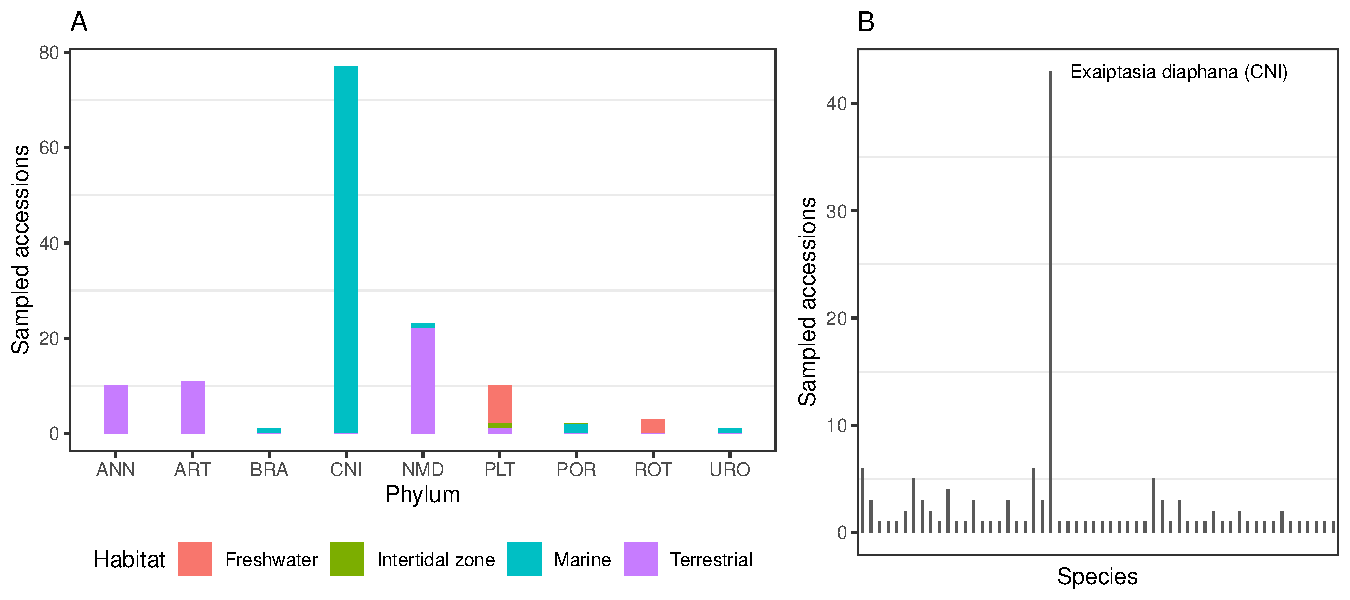
\includegraphics{_main_files/figure-latex/sample50freq-1.pdf}

\caption{Distribution of all 138 sampled accessions across (\textbf{B}) species, (\textbf{A}) phyla and habitats (Pilot). \label{fig:sample50freq}}
\textbf{A.} Most of the sampled accessions belong to annelids, arthropods, nematodes, platyhelminths and, especially, cnidarians. Meanwhile, only one to three accessions have been sampled from Brachiopoda, Porifera, Rotifera and Urochordata. This also occurs for habitat factor, with marine and terrestrial habitats being the most prevalent. There is a unique habitat per phylum except for nematodes and platyhelminths. \textbf{B.} While most of sampled species are represented by one to six accessions, cnidarian species Exaiptasia diaphana accounts for nearly one third of the total number of accessions. It is problematic to consider the accessions of this species as independent members of Cnidaria for belonging to the same species and, most of them, to the same BioSample (SRS742511).

\end{figure}

\hypertarget{kaiju-results}{%
\subsection{Kaiju results}\label{kaiju-results}}

\hypertarget{description-and-univariate-analysis-of-diversity}{%
\subsubsection{Description and univariate analysis of diversity}\label{description-and-univariate-analysis-of-diversity}}

Using RVDB as a database and an E-value threshold of \(0.01\), 76 viral families were identified for all 138 datasets. 24 of these families have less than 10 reads assigned among all samples. Alternatively, 18 viral families are found only in a particular sample. In contrast, other families are much more consistently found: \emph{Mimiviridae} (in \(98\%\) of the samples), \emph{Herpesviridae} (\(96\%\)), \emph{Poxviridae} (\(95\%\)), \emph{Retroviridae} (\(93\%\)), \emph{Marseilleviridae} (\(84\%\)), \emph{Baculoviridae} (\(84\%\)), etc. Since most of these families harbor dsDNA viruses, this suggests that their RNA transcripts have been identified in almost all samples. The most frequently found RNA virus families are \emph{Hepeviridae} (\(82\%\)), \emph{Flaviviridae} (\(81\%\)), \emph{Partitiviridae} (\(80\%\)), \emph{Nairoviridae} (\(76\%\)), \emph{Reoviridae} (\(73\%\)), etc. Among these families, \emph{Mimiviridae}, \emph{Marseilleviridae} (protists) and \emph{Hepeviridae} (vertebrates) are not reported to infect invertebrates. However, the classification of sequences into these families can be the result of sample contamination by other organisms or a lack of specificity by Kaiju. Still, this is not a problem, since the aim of the study is to characterize the communities of viruses associated to different invertebrates, not only the viruses that are able to infect them, i.e.~the characterization of their metavirome and not only their virome \emph{sensu stricto}.

Also, there is no support to confirm that sequences assigned to families that are known to infect invertebrates belong, in fact, to fully functional viruses, but these transcripts could represent transcriptionally active EVEs. Unclassified viruses, i.e.~virus species without a family assigned, also have to be taken into consideration as a further part of the virome composition, thus reaching up to 77 components. Unclassified viruses were identified in \(94\%\) of the samples and account for \(17.5\%\) of all viral reads, second most predominant component after \emph{Retroviridae} (\(35.1\%\)). It appears that the relative abundance of unclassified viruses is lower in marine invertebrates (Figure \ref{fig:kaijudiv} C).

With reference to the sparsity of the dataset, no viral reads were found in three samples, all belonging to \emph{Exaiptasia diaphana}. Furthermore, nearly \(74\%\) of all cells in the abundance matrix contained zero values. The idea of sparsity is related to \(\alpha\)-diversity (\(F\)), which for each row equals the number of non-zero cells regardless of abundance. For most of the samples, around 23 families were observed (\(IQR\)\footnote{Interquartile range (\(IQR\)): the absolute difference between the third and the first quartiles, which are equivalent to the 75th and the 25th percentiles, respectively.}\(= 26.00 - 19.25\)). In this distribution, outliers are predominantly found in the lower end of the distribution (Figure \ref{fig:kaijudiv} A). The same is the case of Shannon diversity index (\(H^\prime\)) distribution, which takes into account the evenness of the communities (Figure \ref{fig:kaijudiv} B). In this case, observed \(H^\prime\) values lie in the range between 0 and \(2.30\) with median in \(1.73\) and \(IQR = 1.93-1.27\). In the literature, mostly \(H^\prime\) values below 1 have been reported for viromes of vertebrates such as birds \autocite{Geoghegan2021} and viromes of soil samples \autocite{Adriaenssens2017}, both using DIAMOND blastx. So, the default \(0.01\) E-value threshold for Kaiju might be too liberal, causing an overall presence and abundance of false positives in the taxonomic classification. This is aggravated by the effect of library size on the observed diversity without which the distributions for both \(F\) and \(H^\prime\) would lie in higher values: all observations with 15 or less reported families have library sizes of less than 3 Gb (Figure \ref{fig:kaijudiv} D). This suggests a high frequency of sampling zeros among these observations, since their lower diversity is an artifact of an insufficient sequencing depth.

Since unbalanced sample sizes are present in the dataset for phylum and habitat factors, an ANOVA analysis with type III SS can be performed to evaluate the effect of both factors on viral diversity at family level. Building a linear additive model for \(H^\prime\) in function of both factors (reference categories: ANN, Freshwater) and the logarithm of library size (\(log(\)Gb\()\)), only the regression coefficient for \(log(\)Gb\()\) is significant with \(\alpha = 0.05\), indicating that phylum and habitat do not have a significant effect on \(H^\prime\). Very similar results are obtained for \(F\), where \(40\%\) of the variance is explained by \(log(\)Gb\()\) and only the coefficient for nematodes is significantly different from 0. Still, the observed ANOVA \(F\) statistic for the phylum factor results in \(P > 0.05\) in ANOVA and, therefore, the null hypothesis of no differences among phyla prevails.

In summary, these ecological univariate metrics do not appear to be significantly affected by phylum and habitat factors for Kaiju results. Furthermore, specific community structure does not sufficiently describe the virome, since \(H^\prime\) takes into account the distribution of abundances not in a part-specific manner, but just in terms of evenness.

\begin{figure}[!htbp]

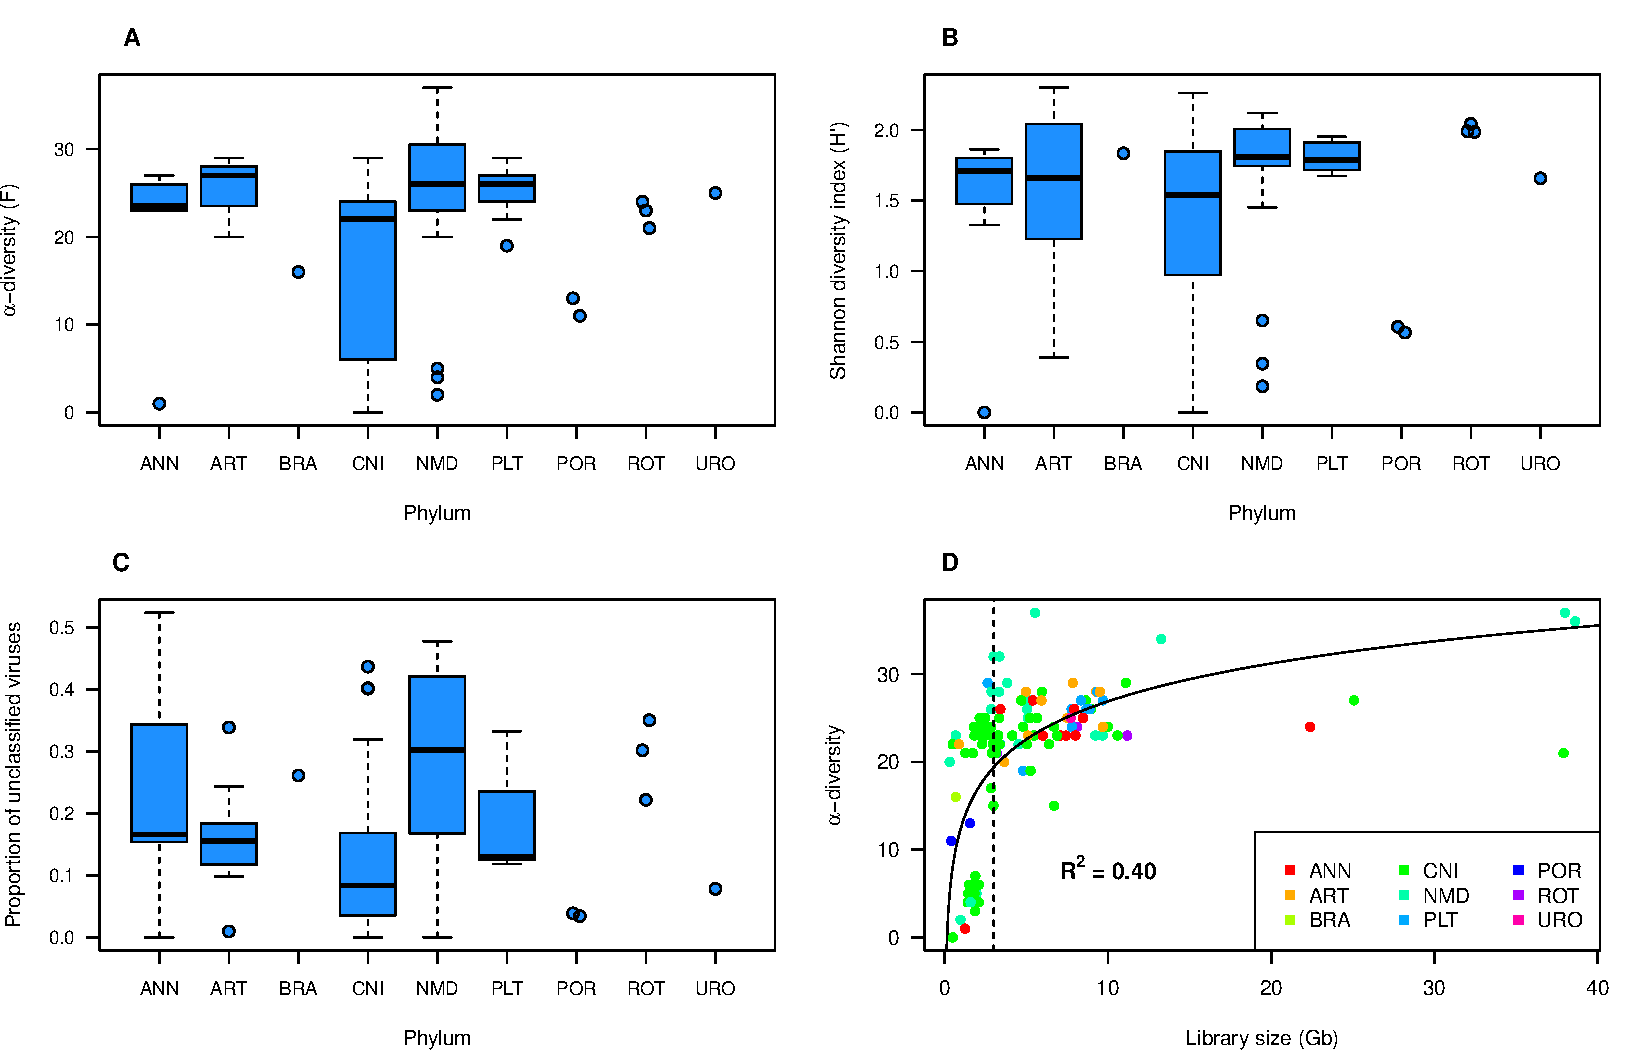
\includegraphics{_main_files/figure-latex/kaijudiv-1.pdf}

\caption{Overview of univariate diversity measures for Kaiju results (Pilot). \label{fig:kaijudiv}}
The distribution of $\alpha$-diversity (\textbf{A}) and H' (\textbf{B}) does not appear to be significantly different between invertebrate phyla. Reported H' is 0 for null observations, although technically it cannot be determined with $F=0$. Limited sample size, the bias introduced by variable library size and a high rate of false positives in the taxonomic classification could have masked true difference between phyla. \textbf{C.} The proportion of unclassified viruses is positively affected by $log($Gb$)$ and is significantly lower in Cnidaria, Porifera and Urochordata ($P < 0.05$, reference: ANN), where all samples are marine. Possibly, the description of novel viruses highly-divergent to accepted families has been more intense in terrestrial than marine environments. \textbf{D.} Viral families richness $F$ is best explained by the logarithm of the bases. A simple linear model including only this covariate explains 40\% of the variance. An arbitrary vertical line has been placed at $3$ Gb to illustrate that the bias introduced by library size is mainly critical for smaller library sizes.

\end{figure}

\hypertarget{permanova-1}{%
\subsubsection{PERMANOVA}\label{permanova-1}}

Before proceeding with PERMANOVA, null observations will be excluded from the analysis. Additionally, the number of samples for \emph{Exaiptasia diaphana} will be reduced to just three observations with largest library size (\(2.7\) - \(3.3\) Gb) to avoid both the overrepresentation of a species and the bias of its low library sizes, resulting in a subset of 98 observations. In the process, two viral families lose their only non-zero observations and, thus, turn uninformative.

The two possible one-way PERMANOVA using phylum and habitat factors were constructed using the Bray-Curtis dissimilarity matrix. In both cases, the observed pseudo \(F\)-statistic supported rejection of \(H_0\) at \(\alpha < 0.05\), thus showing that central locations and/or dispersions do differ among groups. For the simple habitat model, \(12.4\%\) of the variance in the dissimilarity matrix could be explained by habitat differences, while for the phylum model the \(R^2\) statistic reached a value of \(21.8\%\). However, the two-way PERMANOVA including both factors was able to explain nearly \(25\%\) of the variance and the significance of the \(p\)-values was affected by the order of inclusion of factors, i.e.~habitat factor only showed association with differences in location and/or dispersion when added before phylum. In summary, this is indicative of a high degree of collinearity, where most of the differences in the \(BC\) dissimilarity matrix among habitats can be explained by the phylum of the invertebrate host. The classical Akaike Information Criterion (\(AIC\)) was calculated for each model to find if the added complexity offsets the slightly higher goodness of fit. According to \(AIC\), the model with the best selection of variables to explain the generating process of the data was the one-way PERMANOVA with phylum factor (\(AIC_{phyl} = 313.6\); \(AIC_{hab} = 314.7\); \(AIC_{phyl,hab} = 315.4\)). The difference is small between \(AIC\) of both simple models although the phylum model was able to explain almost twice of the variance, since the number of categories is considerably larger for phylum factor.

\begin{figure}[!htbp]

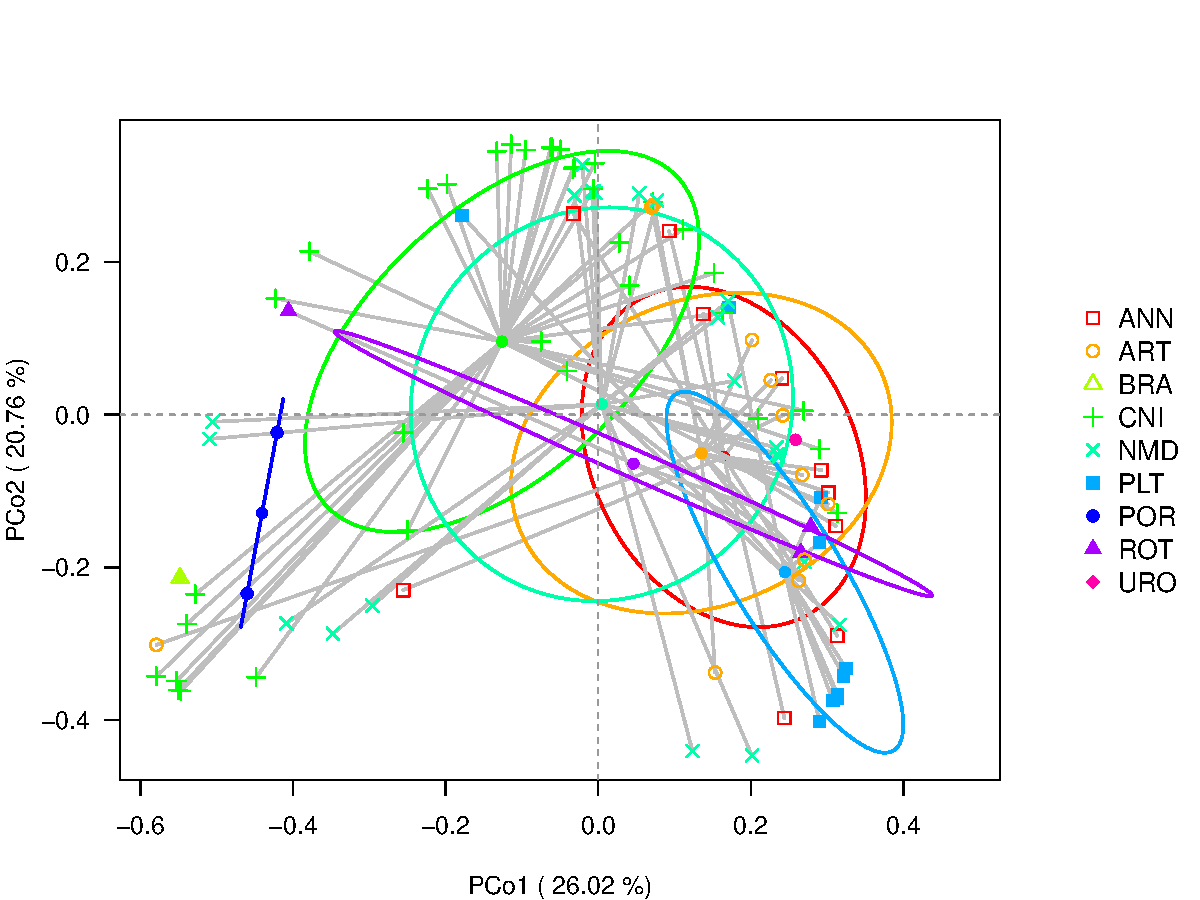
\includegraphics{_main_files/figure-latex/sample50pcoakaiju-1.pdf}

\caption{Principal Coordinate Analysis of Bray-Curtis dissimilarity matrix with Kaiju results (Pilot).\label{fig:sample50pcoakaiju}}
The positions of the samples in the space of the two first principal coordinates are connected to their phylum's central location by grey segments. In this case, medians were computed instead of centroids, which are more sensitive to outliers. Ellipses represent one standard deviation from the group's median. Within-group dispersion is very notable, as, for instance, cnidarian observations are spread across most of the overall dispersion range in the first two principal coordinates. With respect to the differences in the medians of most frequent phyla, viromes of cnidarians (marine) are most distant to those of platyhelminths (mostly freshwater), while viromes of annelids, arthropods and nematodes (mostly terrestrial) lie in between.

\end{figure}

Next, PERMDISP test was performed over \(BC\) to examine if the phylum groupings produced homogeneous within-group dispersions (\(H_0\)). According to this test, homogeneity of group variances can be accepted for the simple phylum model (\(p\)-value\(> 0.05\)), indicating that the rejection of \(H_0\) in PERMANOVA is due to true differences in the central locations between phyla. As a means to visualize location and dispersion across phyla, Principal Coordinates Analysis (PCoA) was performed over the \(BC\) dissimilarity matrix. With this method of metric multidimensional scaling, an Euclidean square matrix of orthogonal columns is obtained, allowing the representation of the observations in a bidimensional space with a limited loss of information. In this case, the first two principal coordinates explained \(46.8\%\) (\(26.0\% + 20.8\%\)) of the variation in the data. This goodness of fit was calculated by the ratio between the sum of the eigenvalue for these two coordinates and the sum of the absolute value of all eigenvalues.

In Figure \ref{fig:sample50pcoakaiju}, observations are represented in the Euclidean space of the first two principal coordinates. Most observations are located in the right quadrants, although some of them are scattered in the left quadrants at a long distance from their phylum's respective median. Medians and dispersion ellipses of arthropods and annelids, both with exclusively terrestrial observations sampled, are very nearly located, suggesting that their average viromes are similar according to Kaiju taxonomic classification. Platyhelminthes samples, mostly freshwater, are fairly separate from cnidarians, except for the single observation of ``Intertidal zone'' habitat, which is ecologically related to marine environments.

Although some interesting observations can be made, the data has a considerable amount of within-group dispersion or \emph{noise} overall. Apart from that, some issues arise for the dataset, namely, \emph{(i)} the inclusion of groups with one or two observations for PERMANOVA and PERMDISP is problematic, since the within-group dispersion is 0 or symmetrical, respectively and \emph{(ii)} although the use of the \(BC\) dissimilarity matrix is fairly well established among microbiome and virome analysts, it does not embrace the compositional nature of the data \autocite{Gloor2017}. Its main drawback is that it is sensitive to scale variation, e.g.~sequencing depth, along with other violations of compositional data principles. Under the compositional framework, the Aitchison distance is preferred for being more stable and satisfying the principles of compositional data.

\hypertarget{kaijusample50}{%
\subsubsection{Compositional PCA}\label{kaijusample50}}

While it has been seen that invertebrate phylum and habitat factors appear to drive differences in the composition of viromes estimated by Kaiju taxonomic classification, it is still unclear which viral families are mainly responsible for this from previous analyses. Preserving the reduced dataset from the previous section, subcompositions of 46 parts were obtained after excluding rare viral families both in occurrence and relative abundance. The frequency of zero values in the resulting matrix was reduced to approximately \(50\%\). Remaining zero values were replaced and \emph{clr} transformation was performed over the imputed dataset. The first two principal components (PC) after SVD were able to summarize around \(32\%\) of the variance between subcompositions. In the scores plot (Figure \ref{fig:sample50biases}, most observations are grouped relatively near 0 for PC2 and spread across the first PC. However, an outlying group is found in extremely negative values for PC2. These observations have either a very low library size or result from DNA-Sequencing experiments, which was not controlled when sampling these SRA accessions.

After filtering out observations with these potential sources of bias, the dimensionality reduction in the parts, sparsity treatment and transformation process was repeated for the remaining dataset of 79 rows. This time, PC1 and PC2 together explained nearly \(36\%\) of the variance in the \emph{clr} coefficients matrix. As for the scores, a similar pattern to that identified for PCoA can be identified: viromes of nematodes are most distant to those of cnidarians, while arthropods and annelids still form a group with a relatively moderate within-group dispersion, although more near to cnidarians (Figure \ref{fig:sample50pcakaiju}. Platyhelminths are notably dispersed, except for six clustered observations that belong to the same species (\emph{Dugesia japonica}).

With respect to loadings, \emph{Reoviridae} and \emph{Asfarviridae} have a prominent influence on PC1 and PC2, respectively. The host range of both families include invertebrates. Abundance of \emph{Reoviridae} (dsRNA viruses) sequences seems to be highly variable between the samples, ranging from \(0\) to \(96\%\) in abundance relative to the whole virome. In the cnidarian samples located in the negative end of PC1, relative abundance of \emph{Reoviridae} sequences is extremely high, suggesting an ongoing infectious state, whether if its host is the cnidarian itself or not. Although \emph{Asfarviridae} is a relatively rare family only found in \(37\%\) of the observations in the final dataset and with a maximum relative abundance of \(0.02\%\), it is able to explain a notable amount of variation for PC2. This family of dsDNA viruses reported to infect invertebrates (arthropods) is almost always absent from cnidarians and consistently found among nematode samples.

Other influential dsDNA virus families include \emph{Ascoviridae}, \emph{Nimaviridae}, \emph{Alloherpesviridae} and \emph{Adenoviridae}. Of those, \emph{Ascoviridae} (insects) and \emph{Nimaviridae} (aquatic arthropods) are known to infect invertebrates. \emph{Alloherpesviridae} is a family of viruses of fishes and amphibians which seems to be specially dominant in the group of cnidarians with lowest \emph{Reoviridae} relative abundance. \emph{Rhabdoviridae} family harbors ssRNA viruses with a remarkably wide host range among eukaryotes, including invertebrates such as arthropods and nematodes. In fact, rhabdoviruses are only found in arthropods and nematodes in a relative abundance higher than \(0.01\%\) in this dataset. However, plant and vertebrate rhabdoviruses could also contribute to this abundance, since arthropods and nematodes frequently form tight ecological relationships with these organisms.

Among these families, there is an overall higher presence of DNA viruses. Furthermore, there is a large difference in the known diversity of these families. For instance, while only one virus of \emph{Nimaviridae} is known, tens or hundreds of viruses of \emph{Adenoviridae}, \emph{Reoviridae} and \emph{Rhabdoviridae} are identified.

The main strength of Kaiju taxonomic classification is the speed at which the results are obtained without a previous assembly step. Although there is a large amount of within-group dispersion that hinders a clear separation of groups, still most of the highly influential families in the PCA harbor viruses that potentially infect invertebrates, further validating our results. Also, the variations between observations were not necessarily driven by the most consistently abundant families mentioned at the beginning, but also some families of low relative abundance. Besides, library size, library source and single species overrepresentation have been identified as potential sources of bias.

\begin{figure}[!htbp]

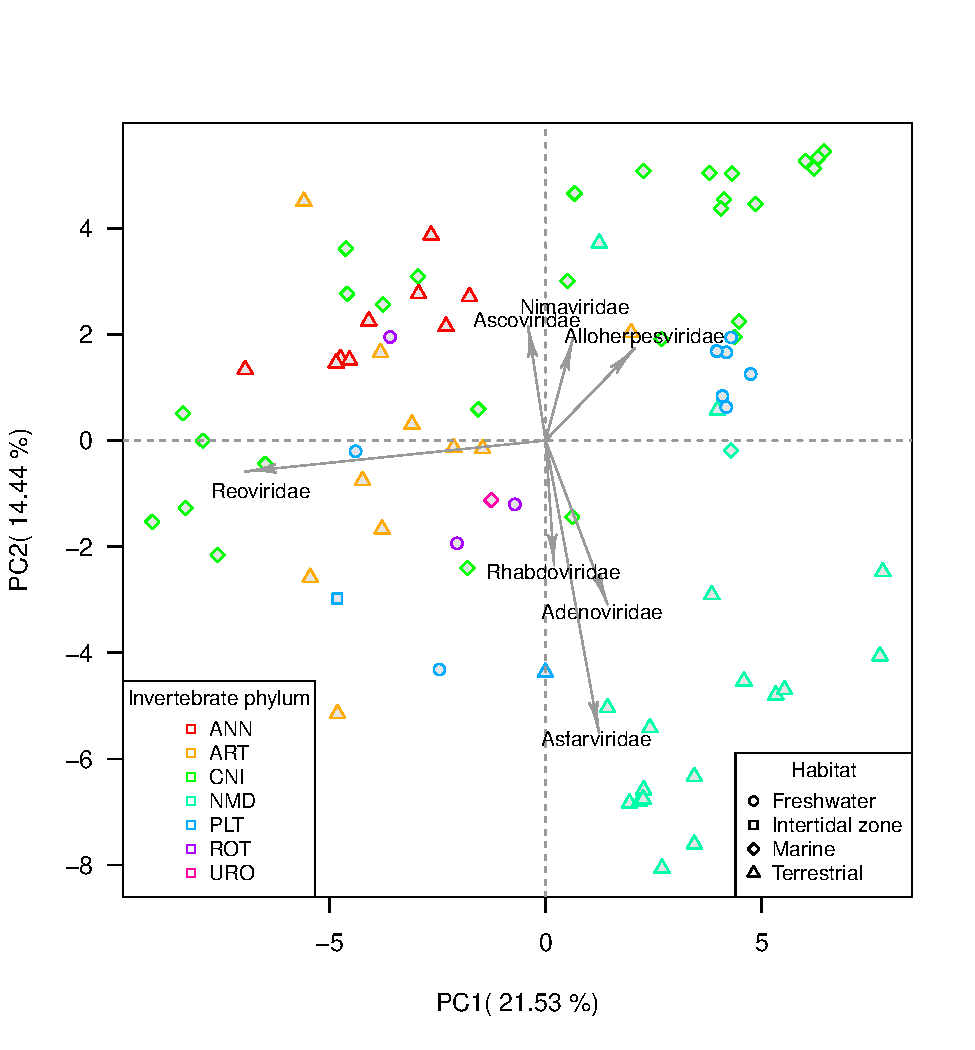
\includegraphics{_main_files/figure-latex/sample50pcakaiju-1.pdf}

\caption{Biplot for Kaiju PCA results (Pilot).\label{fig:sample50pcakaiju}}
Samples with a lower amount of sequenced positions than 2 Gb and 'GENOMIC' library source were excluded from this PCA analysis. Porifera and Brachiopoda phyla were lost in this subset of the data. Furthermore, three of the $46$ viral families were left with only zero values and had to be removed. For the purpose of visualization, loadings vectors were rescaled up to a constant factor and the values on the axes do not correspond with their real values. Only the loadings of the most influential viral families, i.e. with a loadings value higher than $0.2$ in absolute value either for PC1 or PC2, are displayed.
\end{figure}

\hypertarget{diamond}{%
\subsection{DIAMOND}\label{diamond}}

\hypertarget{e90n50pilot}{%
\subsubsection{Description and univariate analysis of diversity}\label{e90n50pilot}}

As a first comment for all contig-related pipelines, the average E90N50 statistic among the assemblies was 1368 bp, which indicates that half of \(90\%\) of the most abundant transcripts are covered by contigs shorter than this value. As for dispersion, central \(50\%\) of calculated E90N50 were in the range between 924 bp and 1791 bp (\(IQR = 867\)). The estimated E90N50 values for other Trinity \emph{de novo} assembled transcriptomes of invertebrates in the literature (2125-2400 bp for terrestrial arthropods \autocite{Li2022,Oppenheim2018}, 1346-3241 bp for marine cnidarians \autocite{Ashwood2021}, 1042-1943 for marine bryozoans \autocite{Treibergs2020}) are usually higher than in most of our assemblies. There seems to be a positive yet very slight correlation between library size and E90N50 (\(P < 0.05\), \(R^2=0.07\)), but this is not enough to explain the overall low values for E90N50. E90N50 statistic also seems to be notably variable depending on the tissue that is sampled and sequenced \autocite{Treibergs2020}. However, most of the observed E90N50 values are still acceptable, since contigs of a few hundred bp are able to summarize the information of several reads. Also, the number of transcripts that account for \(90\%\) of expression within the assembled transcriptomes appears to be highly variable, ranging from just around 5.500 different transcripts to more than 240.000 and with median around 31.000. Apart from the sheer number of unique transcripts, this is also affected by the degree of balance between the expression of the different genes within each sample.

After running taxonomic classification of contigs with DIAMOND, no significant viral hits were found for two samples of Annelida and Cnidaria (\(1.25\) and \(3.36\) Gb, respectively). For the 23 remaining non-null observations of 16 invertebrate species, the estimated concentration of viral transcripts with respect to the whole transcriptome is in the range of \(0.02\%\) to \(0.7\%\) with median of \(0.07\%\). 67 different viral families were identified in total, with an average \(\alpha\)-diversity of 17 families per non-null accession. Estimated \(\alpha\)-diversity seems to be similar both in location and dispersion to that determined with Kaiju results after filtering out null observations and observations with low sequencing depth and genomic library source (79 observations \(\times\) 46 families): while for DIAMOND a range between 8 and 34 is observed with an \(IQR = 19 - 15\), estimated \(\alpha\)-diversity indices had an average of 15 families ranging from 10 to 31 and with \(IQR = 17 - 13\) for Kaiju. Furthermore, the distribution for \(\alpha\)-diversity is relatively homogeneous across all three phyla examined with DIAMOND. Alternatively, estimated Shannon diversity indices were not significantly different between phyla (\(P > 0.05\)) and were distributed mainly between \(1.5\) and \(2\), which is consistent with Kaiju results.

Regarding the identified families and their relative abundances in the compositions, now the most abundant category is that of unclassified viruses with an average \(19\%\) of viral transcripts among the samples. Next, sequences of \emph{Adintoviridae}, which were not a specially abundant family under Kaiju results, are found in an average relative abundance of \(16.8\%\). Adintoviruses are a group of animal dsDNA viruses related to adenoviruses and baculoviruses that are able to undergo integration into the host genome \autocite{Starrett2021}. dsDNA virus families dominate the dataset in terms of abundance: the most abundant RNA virus family (\emph{Iflaviridae}, a family of insect-infecting viruses, with \(4.4\%\) of viral transcripts) is surpassed by six dsDNA virus families, including viruses of protists (\emph{Mimiviridae}, \(11.5\%\); \emph{Phycodnaviridae}, \(6.1\%\)), viruses of animals (\emph{Poxviridae}, \(6.4\%\); \emph{Iridoviridae}, \(5.7\%\)) and bacteriophages (\emph{Myoviridae}, \(4.8\%\)). 20 viral families are found just in one of the samples, while 11 are found at least in half of the virome compositions, including an ubiquitous presence of unclassified viruses and adintoviruses. With regards to the overall sparsity in the compositional matrix, \(74\%\) of its entries are zero values.

\hypertarget{permapilot}{%
\subsubsection{PERMANOVA}\label{permapilot}}

Since in this case the interaction between phylum and habitat yields three categories, there is only the option to perform one-way PERMANOVA tests. Both possible models show significant association (\(P < 0.05\)) of phylum and habitat factors to any differences in location or dispersion among the groups. However, phylum model is able to explain \(30.5\%\) of the variance in the \(BC\) matrix while habitat model only reached an \(R^2\) of \(17.5\%\). The superior fit of the phylum model can also be seen from its inferior AIC (\(40.6\) vs.~\(42.6\)). PERMDISP test showed evidence for the rejection of the homogeneity of within-group dispersion among groups hypothesis (\(P < 0.05\)), suggesting that it is unclear if the rejection of \(H_0\) in PERMANOVA is due to true location differences between groups. As a means of comparison, PERMANOVA and PERMDISP analyses were also performed over the Aitchison distances matrix after replacement of zeros, resulting in the same combination of hypotheses testing decisions. Again, variance explained by phylum factor was approximately \(30\%\).

Aiming to visualize the location and dispersion within and between phyla for both cases, representation of the two first principal coordinates was performed (Figure \ref{fig:sample50pcoadiamond}. It seems that for both matrices, but especially for the Aitchison distances matrix, PCo1 and PCo2 capture a difference in central locations among phyla. Therefore, average virome compositions apparently differ between phyla and habitats for this very reduced dataset. The heterogeneity of variances is also clearly visible, especially between cnidarians and the rest of groups. The low within-group variation recorded for cnidarians might be a sampling artifact due to the presence of only two species, with one of them carrying four out of five observations. Using the Aitchison distances, the observed range of PCo1 and PCo2 shows no overlap between groups. Such is the resolution in the segregation of groups that a simple clustering algorithm like \(k\)-means fully reconstructs habitat division with \(k = 2\) (annelids grouped with arthropods). With \(k = 3\), clusters reproduce the original phylum division, except for an arthropod observation that groups with annelids. In conclusion, Aitchison distances have shown significant practical advantages in this case, apart from its theoretical superiority in the study of dissimilarities between compositions.

\begin{figure}[!htbp]

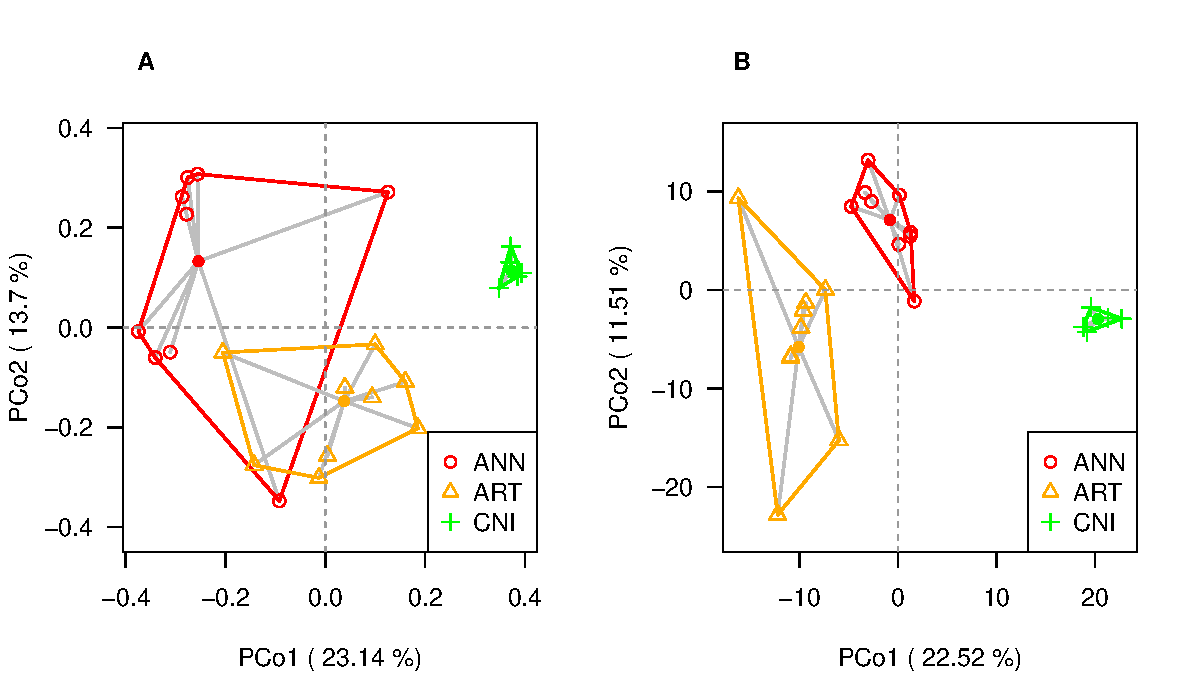
\includegraphics{_main_files/figure-latex/unnamed-chunk-8-1.pdf}

\caption{Principal Coordinate Analyses for DIAMOND results (Pilot).\label{fig:sample50pcoadiamond}}
PCoA was performed over the Bray-Curtis dissimilarities matrix (\textbf{A}) and the Aitchison distances matrix (\textbf{B}) for the 23 non-null compositions obtained from DIAMOND taxonomic classification of contigs. Observations are connected to the median of their phylum with grey segments. The convex hull is displayed for each phylum to show the range of the observed individuals of each phylum in the space of PCo1 and PCo2. Convex hulls show no overlap between phyla in the case of using Aitchison distances, resulting in a segregation of groups of high resolution. In both cases, PCo1 accounts for most of the differences between phyla and, especially, between habitats.

\end{figure}

\hypertarget{compositional-pca}{%
\subsubsection{Compositional PCA}\label{compositional-pca}}

PCA was performed over the same \emph{clr} coefficients matrix used for PCoA analysis with Aitchison distances. Accordingly, the distribution of scores in the bidimensional space of the two first PCs is very similar to that observed in the previous section. It is worth mentioning that, in this case, no exclusion of rare families was made before non-parametric replacement of cells with tpm \(< 0.001\), ergo all zeros are assumed to be sampling zeros. Roughly \(34\%\) of the variance was explained by PC1 (\(22.5\%\)) and PC2 (\(11.5\%\)). Different phyla are mainly separated by PC1, which also captures the habitat division (Figure \ref{fig:sample50pcadiamond}). PC2 helps in the separation of annelids and arthropods, which share terrestrial habitat. Therefore, viral families that contribute the most to PC1 are responsible for the habitat division of viromes, while the phylum division requires the interpretation of most influential families to both PC1 and PC2. Also, PC3(\(9.4\%\)) was seen not to segregate phyla, but to capture a great amount of within-group dispersion, especially for arthropods, similarly to PC2.

As to the loadings vectors, the most influential families are relatively balanced in terms of effect to PC1 and PC2, i.e.~there is not a single family with a loadings vector much higher in norm than the rest. It can be concluded that the viromes of cnidarians are rich in DNA viruses of archaea, bacteria (\emph{Microviridae}, \emph{Podoviridae}) and protozoa (\emph{Marseilleviridae}, \emph{Pithoviridae}) with respect to the the viromes of annelids and arthropods. Also, the relative abundance of ascoviruses, which are dsDNA viruses of insects, appears to be greater in cnidarians than in arthropods or annelids. This could respond to the presence of non-described viruses related to \emph{Ascoviridae} in cnidarian samples. Viromes of arthropods seem to be particularly rich in ssRNA virus families of eukaryotes, such as \emph{Dicistroviridae}, \emph{Iflaviridae} and \emph{Rhabdoviridae}. The first two of these families are related to each other and only known to infect arthropods. Nevertheless, sequences of \emph{Parvoviridae}, which is a family of DNA viruses of animals, including diverse invertebrates, also seem to be specially frequent in arthropods. Families found in differentially greater proportion in annelids are more diverse, including dsDNA bacteriophages (\emph{Siphoviridae}), retroviruses and viruses of arthropods (\emph{Baculoviridae}, \emph{Polydnaviridae} and \emph{Nairoviridae}). It remains unknown if any member of these three families are able to infect annelids or their detection has just been a consequence of the tight ecological relationship of annelids with soil-inhabiting arthropods, including eggs and larvae of many insects.

In conclusion, we note that the viral families associated with a group of invertebrates tend to be either: \emph{(i)} able to infect members of said invertebrate group or \emph{(ii)} part of the virome of microbes found when sampling said invertebrates. This implies both a host taxonomic effect that is summarized here by phylum factor and a habitat effect. Again, it is important to mention that identified sequences do not necessarily belong to replicative viruses, but could result from EVE expression. While it is true that a very reduced dataset was used with DIAMOND, within-group distances are moderate for phylum and habitat groupings and make possible cluster partitioning, in contrast to Kaiju results. With DIAMOND, the interpretation of the results seems to be relatively coherent with the recognized host range of the viral families.

\begin{figure}[!htbp]

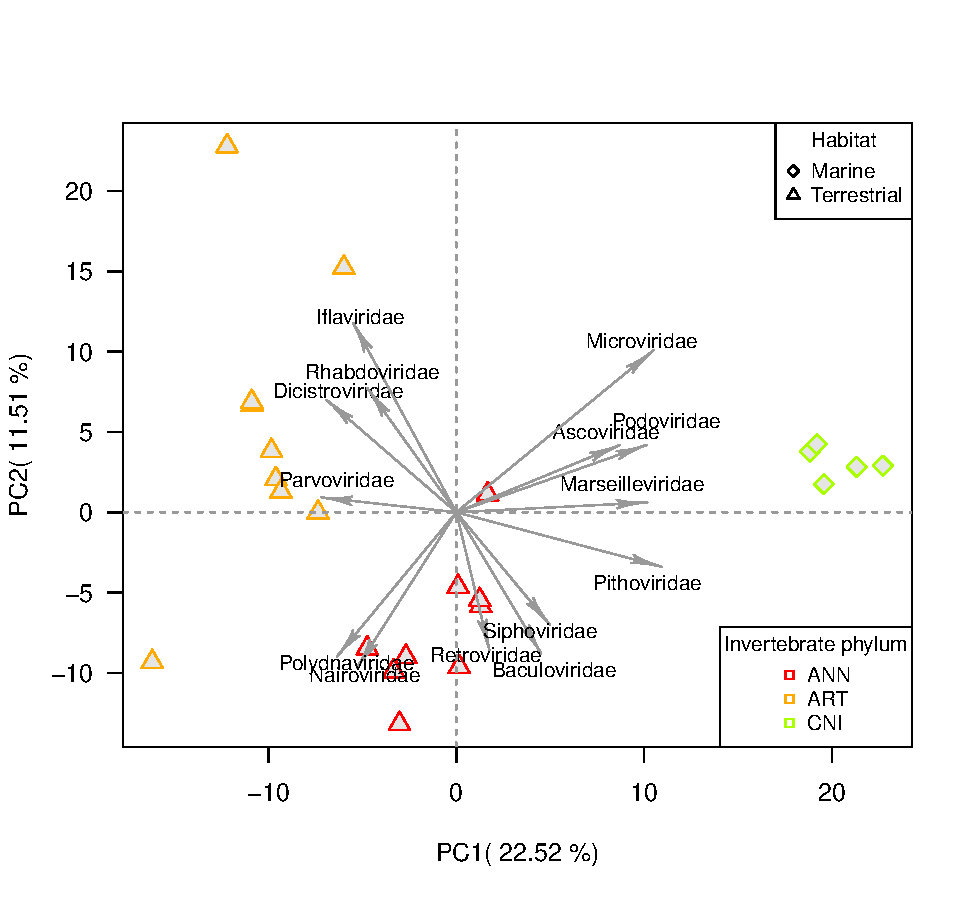
\includegraphics{_main_files/figure-latex/unnamed-chunk-9-1.pdf}

\caption{Biplot representation of PCA for DIAMOND results (Pilot).\label{fig:sample50pcadiamond}}
PCA was performed over the 23 non-null compositions obtained after DIAMOND taxonomic classification transformed to $clr$ coefficients. The variance of the $clr$-transformed parts was not standardized prior to SVD. PC1 and PC2 explain roughly $20\%$ of the standard deviation for all 67 viral families identified with DIAMOND. Loadings vectors with any element in PC1 or PC2 higher than 0.2 in absolute value are represented along with their respective viral families names. 

\end{figure}

\hypertarget{comments-on-the-rest-of-the-contig-analysis-tools-used}{%
\subsection{Comments on the rest of the contig analysis tools used}\label{comments-on-the-rest-of-the-contig-analysis-tools-used}}

\hypertarget{virfinder-and-virsorter2}{%
\subsubsection{VirFinder and VirSorter2}\label{virfinder-and-virsorter2}}

Ideally, VirFinder and VirSorter2 should provide a preselection of putatively viral contigs, so that only contigs that are true positives in DIAMOND taxonomic classification are preserved. Additionally, these binary classifiers use variables other than sheer sequence similarity that could prevent the occurrence of false positives.

Using VirFinder, approximately \(20\%\) of contigs were classified as viral (\(FDR < 0.05\)), which would only reduce DIAMOND's workload and runtime to a fifth. However, only 49 different viral families are identified for the 23 non-null observations, which translates to a loss of 18 viral families with respect to the DIAMOND analysis without the preselection step. These results might indicate that some true viral sequences present in the sample are lost in VirFinder step or that VirFinder excludes non-viral contigs that are classified as viral by DIAMOND. An anomalous behavior was observed in the distribution of \(p\)-values obtained through VirFinder classification of contigs: \(p\)-values (and \(FDR\)) showed a tendency to oscillate around the significance threshold as the contig length increased (Figure \ref{fig:vfpvals}). Assuming that two populations of contigs coexist within the whole, i.e.~those viral and those non-viral, it would be expected that the distribution of \(p\)-values for the non-viral contigs would be uniform {[}0,1{]}. However, as the contig length increases, the range of observed \(p\)-values contracts more and more around \(FDR \sim 0.05\), while longer sequences carry more information to accept or reject the hypothesis of viralness (\(H_1\)). Apart from this, the resolution in the segregation of groups in PCA has decreased significantly with respect to DIAMOND classification alone (Figure \ref{fig:sample50pcavfvs2} A). Therefore, contigs of viral families that drive phylum and habitat differences between observations have been classified as non-viral by VirFinder model, overall increasing the within-group dispersions.

In contrast, VirSorter2 just roughly classifies \(0.07\%\) of contigs as viral. As a result, only 29 different viral families are found and three more samples become null observations. While a high proportion of those sequences are then classified into viral families by DIAMOND, this step greatly reduces the total number of viral contigs after the pipeline. However, it is able to capture the differential information of each group and approximately reproduce what has been seen in the DIAMOND analysis, where generally the same viral families influence the segregation of the data in similar ways (Figure \ref{fig:sample50pcavfvs2} B). Also, the overall abundance of viruses with uncertain family assignation increases to approximately \(47\%\) of all viral transcripts after using the VirSorter2 pipeline. In summary, VirSorter2 seems to be less problematic than VirFinder, although neither of these models has been intensively trained with invertebrate datasets.

\hypertarget{cat}{%
\subsubsection{CAT}\label{cat}}

Out of 131 transcriptome assemblies, CAT was able to annotate at least one contig as viral for only 95 samples. Overall, contigs of 54 different viral families were recorded at least once, which reflect a lower diversity compared to Kaiju or DIAMOND. An exceptionally high presence of zeros in the compositional matrix was observed: \(93.5\%\) before excluding null observations and \(92.2\%\) afterwards. However, after filtering out problematic observations with low library size and non-transcriptomic library source as in \ref{kaijusample50}, more meaningful results are obtained with reference to Kaiju (Figure \ref{fig:sample50pcacat} A), although only 70 observations and 49 families remain in a matrix with \(89\%\) of zeros. Viromes are apparently divided by habitat in PC1, with arthropods and nematodes being the most distant from cnidarians and aquatic platyhelminths, while annelids lie spread out in between. PC2 appears to originate phylum divisions within the terrestrial (negative quadrants of PC1) and aquatic (positive quadrants of PC1) groupings. As for the loadings, dsDNA viruses of microbes and animals seem to be more dominant in viromes of aquatic invertebrate samples, while RNA viruses of animals are more prevalent in terrestrial samples. In general, the accuracy of the results seems notably superior to Kaiju's and comparable to that seen for DIAMOND blastx-related pipelines. It remains unknown if the recorded loss of diversity of CAT results with respect to DIAMOND corresponds mostly to the occurrence of false positives using DIAMOND or false negatives using CAT.

\hypertarget{hmmer-cat}{%
\subsubsection{HMMER-CAT}\label{hmmer-cat}}

For this pipeline, contigs have to first show homology to the provided RdRp profiles and, then, to any viral sequence in the reference database used in CAT analysis. A very low number of hits, if any, were obtained for all contigs in \texttt{hmmsearch}. Only 12 observations had non-zero sum compositions and eight of them had more than one viral family present, generally two. Furthermore, only 14 viral families were found at least once. A compositional analysis of this dataset seems rather inappropriate for its extreme sparsity (\(98.2\%\) of all cells). Apart from that, some of the identified contigs with ORFs homologous to RdRp were then assigned to DNA virus families by CAT, which is an undesirable behavior given that RdRp is a characteristic gene of RNA viruses.

\hypertarget{conclusions}{%
\section{Conclusions}\label{conclusions}}

In this pilot test, five different pipelines for taxonomic classification of viruses into families have been compared in terms of time efficiency and results. Overall, Kaiju is the least computationally demanding taxonomic classifier tested. It performs the analysis quickly after the download and preprocessing step. However, its results show a greater amount of \emph{noise}, i.e.~information that does not seem to be related to phylum or habitat groupings, compared to DIAMOND-related pipelines, although establishing a more strict E-value threshold could help improve this situation.

Regarding the four remaining pipelines that use contigs as input, HMMER-CAT is the fastest, but also the least informative one, although a more thoughtful selection of profiles could enhance its results. CAT offers a great alternative to DIAMOND blastx in terms of runtime, since not all possible reading frames of contigs are analyzed, but just the ORFs predicted with Prodigal. VirFinder and VirSorter2 greatly differ in the proportion of predicted viral contigs, with VirFinder being far too unspecific in the classification. As a result, the runtimes of their pipelines are similar, with VirFinder being faster but not providing a very reduced subset of contigs and VirSorter2 being fairly slow by its own, although greatly reducing subsequent DIAMOND analysis workload. Taxonomic classification of all contigs with DIAMOND blastx represents the slowest pipeline and, arguably, the most sensitive of them all.

Apart from this, several sources of bias that were not controlled when sampling the observations for this pilot test have been identified. Namely, the library size and the source of the library, i.e.~the type of nucleic acids sequencing experiment that was applied, showed an effect on the characterized viromes. Samples with library sizes less than \(4\) Gb tend to be associated with viromes with lower \(\alpha\)-diversity, which suggests an insufficient sequencing depth necessary to detect rare-occurring viruses in the transcriptomes. Also, another source of bias is related to the overrepresentation of single species or genera within phyla. The transcriptomes of samples with close taxonomic relationships are naturally similar, but also because they are frequently sampled by the same researchers using the same experimental conditions. For these two reasons, it is problematic to consider all observations of a phylum as independent members, regardless of their taxonomic affiliations below this rank. The ideal solution would be to include the whole phylogenetic dependence structure that connects not only the species within a phylum, but also phyla to each other, instead of the use of independent or nested factors for each considered taxonomic rank.

As for the results, the use of Aitchison distances and Bray-Curtis dissimilarities was compared for PERMANOVA and PERMDISP tests and PCoA. Regardless of Aitchison distances showing more meaningful results, it has been recently argued that their application might be more appropriate for community composition studies than traditional Bray-Curtis dissimilarities, which are sensitive to scale effects. The families that differentiate the most observations of different phyla and habitats can be identified in the biplot representations of PCA. Other representations, such as heatmaps and barplots can be used to examine the relative abundances of each viral family in the observations or aggregations by group, although this will be reserved for the definitive analysis.

\hypertarget{definitive-analysis}{%
\chapter{Definitive analysis}\label{definitive-analysis}}

\hypertarget{lessons-learned-from-the-pilot-test}{%
\section{Lessons learned from the pilot test}\label{lessons-learned-from-the-pilot-test}}

\hypertarget{avoiding-sources-of-bias}{%
\subsection{Avoiding sources of bias}\label{avoiding-sources-of-bias}}

Three strategies are proposed to reduce the dataset in order to avoid biases in the data and/or to maximize the information we can obtain from a limited number of observations. Firstly, all genomic DNA or small RNA sequencing experiments are excluded from the analysis and only second generation transcriptomic sequencing experiments (RNA-Seq) are preserved. This produces a loss of 1108 accessions and 67 species.

Secondly, it has been shown that estimated virome diversity is highly affected by library size, especially in the range of 0 to 3 Gb (Figure \ref{fig:kaijudiv} D). This arbitrary delimitation (3 Gb) based on the seemingly logarithmic relationship between library size and \(\alpha\)-diversity tries to avoid the most critical phase of this function, while keeping the observations that lie in the more stationary part, where we assume that sequencing depth differences do not play a major role. In this trade-off situation, a more conservative delimitation would induce a more noticeable decline in the number of species and increase the average processing time per accession. This decision produces a further decrease in the number of species to 31 and a much sharper loss of accessions from 31608 to just 6754. Moreover, accessions with an SRA file of 20 or more GB were put in a low priority because of the expected decrease in the speed of their processing and their low added information value with respect to experiments of more moderate library size. Importantly, all 32 phyla are still represented by one or more observations.

Lastly, it has been noted that random sampling of accessions can result in a very uneven exploration of species. The overrepresentation of some species can bias the virome compositions that are estimated for certain phyla and underestimate the diversity of viromes within groups. In order to maximize the exploration of invertebrate viromes in the dataset while processing as few observations as possible, a single accession was randomly sampled for each unique species. However, different genera, families or orders can still be asymmetrically explored within a phylum and thus, it cannot be assumed that phyla are explored in a completely balanced way. In the end,
1508 accessions of unique species are kept for the analysis. Since this is an objective for the long term, in this definitive analysis phyla with less than 30 observations are prioritized for a more complete analysis, while only five species are sampled from majoritary phyla, i.e.~Annelida, Arthropoda, Cnidaria, Echinodermata, Nematoda, Platyhelminthes and Porifera (Table \ref{tab:deftab}).

\begin{table}[!h]

\caption{\label{tab:deftab}Number of sampled species per phylum in the definitive analysis after avoiding sources of bias.}
\centering
\resizebox{\linewidth}{!}{
\begin{tabular}[t]{lclc}
\toprule
Phylum & Unique species & Phylum & Unique species\\
\midrule
\cellcolor{gray!6}{Annelida (ANN)} & \cellcolor{gray!6}{5} & \cellcolor{gray!6}{Micrognathozoa (MIC)} & \cellcolor{gray!6}{1}\\
Arthropoda (ART) & 5 & Mollusca (MOL) & 27\\
\cellcolor{gray!6}{Brachiopoda (BRA)} & \cellcolor{gray!6}{7} & \cellcolor{gray!6}{Nematoda (NMD)} & \cellcolor{gray!6}{5}\\
Bryozoa (BRY) & 9 & Nematomorpha (NMM) & 3\\
\cellcolor{gray!6}{Chaetognatha (CHA)} & \cellcolor{gray!6}{10} & \cellcolor{gray!6}{Nemertea (NME)} & \cellcolor{gray!6}{14}\\
Cnidaria (CNI) & 5 & Onychophora (ONY) & 25\\
\cellcolor{gray!6}{Ctenophora (CTE)} & \cellcolor{gray!6}{21} & \cellcolor{gray!6}{Orthonectida (ORT)} & \cellcolor{gray!6}{1}\\
Cycliophora (CYC) & 3 & Phoronida (PHO) & 4\\
\cellcolor{gray!6}{Dicyemida (DIC)} & \cellcolor{gray!6}{2} & \cellcolor{gray!6}{Placozoa (PLA)} & \cellcolor{gray!6}{3}\\
Echinodermata (ECH) & 5 & Platyhelminthes (PLT) & 5\\
\cellcolor{gray!6}{Entoprocta (ENT)} & \cellcolor{gray!6}{3} & \cellcolor{gray!6}{Porifera (POR)} & \cellcolor{gray!6}{5}\\
Gastotricha (GAS) & 1 & Priapulida (PRI) & 3\\
\cellcolor{gray!6}{Gnathostomulida (GNA)} & \cellcolor{gray!6}{1} & \cellcolor{gray!6}{Rotifera (ROT)} & \cellcolor{gray!6}{15}\\
Hemichordata (HEM) & 3 & Tardigrada (TAR) & 7\\
\cellcolor{gray!6}{Kinorhyncha (KIN)} & \cellcolor{gray!6}{1} & \cellcolor{gray!6}{Urochordata (URO)} & \cellcolor{gray!6}{7}\\
Loricifera (LOR) & 1 & Xenacoelomorpha (XEN) & 14\\
\midrule
\cellcolor{gray!6}{-} & \cellcolor{gray!6}{-} & \cellcolor{gray!6}{Total} & \cellcolor{gray!6}{221}\\
\bottomrule
\end{tabular}}
\end{table}

\hypertarget{pipeline-election-and-modifications}{%
\subsection{Pipeline election and modifications}\label{pipeline-election-and-modifications}}

While taxonomic classification based on reads with Kaiju using the RVDB database has shown to be very fast, the use of DIAMOND for taxonomic classification of contigs on the nr database significantly slows down the pipelines. However, results of DIAMOND-related pipelines appear to minimize within-group dispersion, possibly due to a lower rate of false positives in the classification of sequences, and so, groups are separated with higher resolution. In the pilot test, sequences that did not have any viral hits were ignored and those sequences that had both host and viral hits were considered viral if the E-value was lower than the specified threshold, even if an eukaryotic or prokaryotic protein showed an even lower E-value. Since only viral hits are taken into consideration, the use of the whole nr database is not justified and only makes pipeline runtimes longer. For this definitive analysis, the nr database was restricted to only viral sequences (Viruses, taxid: 10239), greatly reducing the number of comparisons that must be made for each contig. Although VirSorter2 before DIAMOND and CAT has shown good results and was faster than DIAMOND with blastx option alone, the reduction of the nr database allowed DIAMOND blastx to be applied directly to all assembled contigs in a scalable way. Only two pipelines are maintained for the definitive analysis: \emph{(i)} Kaiju will still be used for the low added runtime it constitutes, but now with an E-value threshold of \(1e-05\) as in DIAMOND and \emph{(ii)} DIAMOND blastx in \texttt{--very-sensitive} mode against viruses in the nr database will be used for contigs as it is expected to provide more meaningful results. An overview of this workflow is shown in Figure \ref{fig:pipeline}. However, only DIAMOND results will be presented.

\begin{figure}[!htbp]

\begin{center}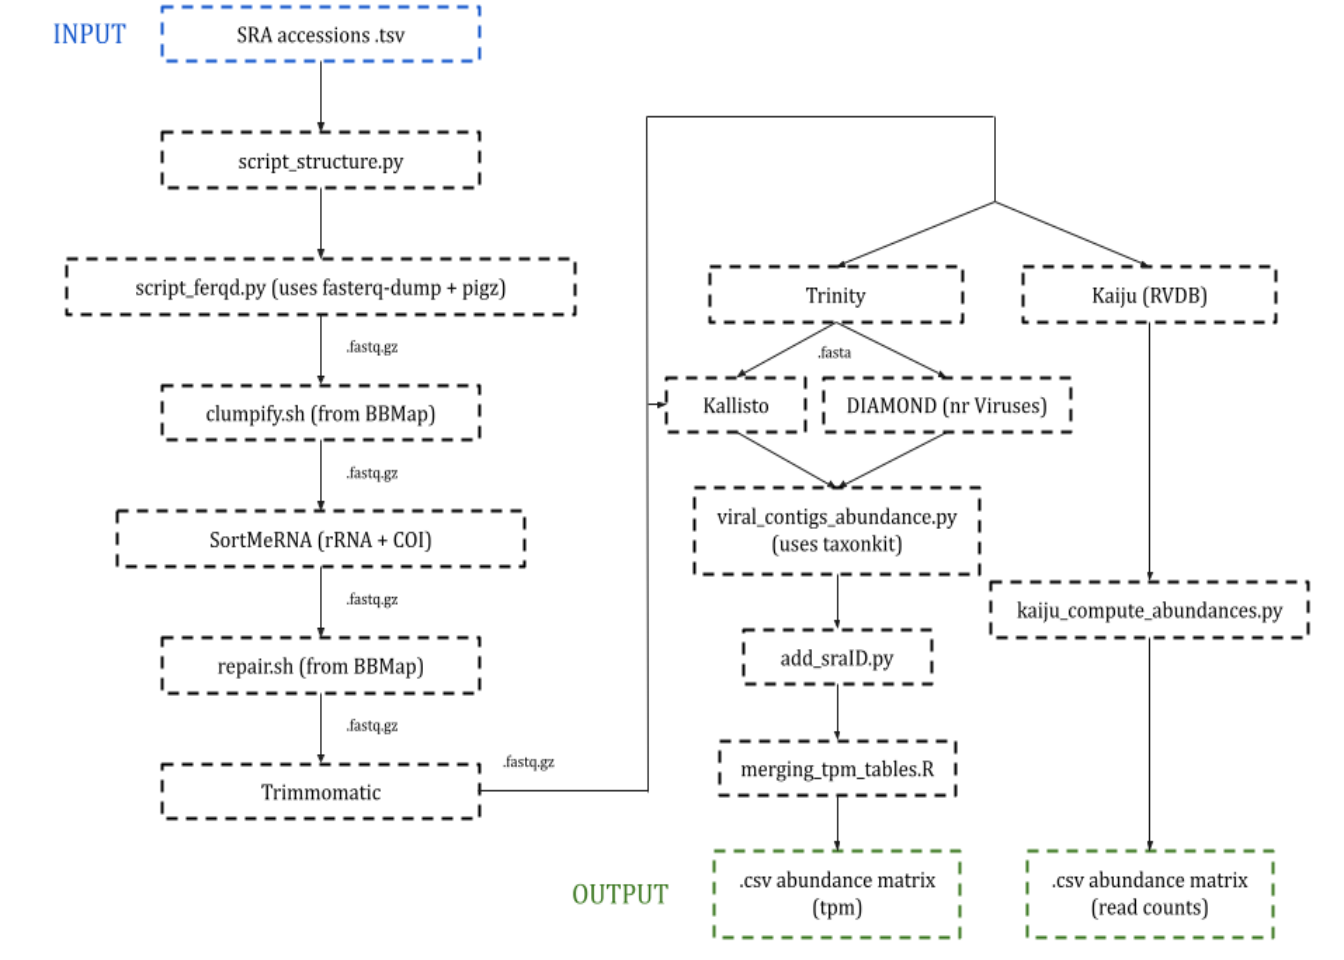
\includegraphics{_main_files/figure-latex/pipeline-1} \end{center}

\caption{Overview of programs used for detection of viruses in the definitive analysis. \label{fig:pipeline}}
The global pipeline bash script and individual \emph{ad hoc} python and R scripts can be accessed in the GitHub repository of this project \href{https://github.com/palf98/metaviromics}{(https://github.com/palf98/metaviromics)}. The original collection of accessions are also provided to allow for reproducibility of methods.
\end{figure}

Even if taxonomic classification of contigs has been sped up, the assembly step still requires a notable amount of time. In the part of the pipeline where reads are preprocessed, some additional steps can be used to reduce the number of reads that have to be compared in the downstream analyses. First, second generation sequencing is known to produce duplicates, i.e.~the same original nucleic acid molecule is identified as two or more identical reads, for a series of reasons, which include PCR, optical and clustering artifacts. Thus, exact duplicate reads arise in NGS libraries due to the limitations of the sequencing methods. The removal of exact duplicates can lead to a loss of more than \(30\%\) of the total reads, without the alteration of the accuracy in the identification of individual sequences \autocite{Ebbert2016}. In this case, \texttt{dedupe} function of clumpify.sh, included in \href{https://sourceforge.net/projects/bbmap/}{BBMap toolkit} \autocite{Bushnell2014} version 38.96 was used to remove duplicate reads. For single-end reads, exact matches are considered duplicate reads, while for paired-end reads both ends have to match perfectly between multiple pairs. In both cases, one element (single or paired) of each duplicate class is preserved.

Additionally, since the true host sequences are not of interest in the taxonomic classification, the assembly of their reads into contigs is something to avoid in order to improve the efficiency of the pipeline. However, reference genomes, where reads could be mapped and discarded for downstream analyses, are not available for all sampled invertebrates. Therefore, the exclusion of host transcripts has to rely on very conserved genes of invertebrates, which are used as phylogenetic markers, such as rRNA and COI mitochondrial subunits. In this context, rRNA is of special interest since its transcripts account for the majority of molecules within the whole RNA population in animal cells (\(\sim80\%\)). Bioinformatic ribosome depletion of transcriptomes is a common practice in RNA-Seq data analysis and its application to invertebrate datasets has led to similar levels of mRNA molecules as in poly-A enriched sequencing samples \autocite{Kim2019}.

For this purpose, \href{https://github.com/biocore/sortmerna}{SortMeRNA} \autocite{Kopylova2012} (version 4.3.4) was used to filter reads that showed significant similarity to 18S and 28S rRNA subunits of eukaryotes from the default SortMeRNA rRNA database. A custom cytochrome c oxydase (COX) database including subunits of mitochondrial and nuclear genomes of different animals was used alongside rRNA databases and can be accessed in \url{https://github.com/palf98/metaviromics/blob/main/COI.fasta}. SortMeRNA was run in \texttt{--paired-in} mode to keep strictly non-rRNA pairs of reads, i.e.~pairs where one end aligned to rRNA and the other did not were excluded. Therefore, after SortMeRNA analysis step the total transcript population used is constituted predominantly by non-rRNA and non-COX transcripts. Additionally, this step sort of normalizes the libraries even if they originate from different RNA extraction and selection protocols. For instance, the percentages of viral transcripts in the pilot test could be greatly affected by the differential concentration of rRNA transcripts among samples. As a last addition to the pipeline, repair.sh program of BBMap, which tries to find the paired read for each read, was run after SortMeRNA to remove the singletons that SortMeRNA rarely produces and that corrupt the paired relationship in the fastq files.

Bioinformatics methods that were not mentioned in this section were used as described in \ref{pilot-bioinf}. Statistical methods remain the same as described in \ref{pilot-stat}, with the exception of the use of Aitchison distances instead of Bray-Curtis dissimilarities for the PERMANOVA and PERMDISP tests.

\hypertarget{results-1}{%
\section{Results}\label{results-1}}

\hypertarget{pipeline-results-overview}{%
\subsection{Pipeline results overview}\label{pipeline-results-overview}}

First of all, more than \(45\%\) of the total number of reads are discarded jointly in all three preprocessing steps for all samples and in most cases, only 20 to \(36\%\) of reads are preserved for subsequent analyses (Figure \ref{fig:preprocess}). Deduplication with clumpify produces a very uneven filtering of reads between samples, ranging from almost no duplicates found to a decline of approximately \(90\%\) of reads in the most extreme cases. In average, approximately \(32\%\) of reads are filtered out for being exact duplicates of others. Contrary to what would be expected, the proportion of duplicates found in each sample showed no relation to its library size. So, sequencing depth did not produce a higher proportion of exact duplicates.

In average, SortMeRNA produces the biggest reduction of reads among the preprocessing programs: at least half of reads remaining after deduplication are mapped to 18S or 28S eukaryotic subunits of rRNA or COX transcripts. While a further reduction of 50 to \(60\%\) of reads is noted for most samples by using SortMeRNA, in some cases this reduction can be of approximately \(80\%\). The concentration of rRNA in the literature is normally presented in the range of 70 to \(90\%\) of the whole transcriptome. This might suggest that a portion of the rRNA transcripts were not detected and/or were already filtered out in the deduplication step. It can also be inferred from these results that neither experimental ribosome depletion nor poly-A selection were performed over these datasets, \emph{ergo} it can be assumed that the whole RNA population was surveyed in each sample.

In the case of Trimmomatic, normally more than \(90\%\) of reads have sufficient overall quality scores to be preserved. Although a noticeable global reduction of reads is achieved in the preprocessing steps, \emph{de novo} assembly of contigs with Trinity still uses an important amount of computational resources and time (Figure \ref{fig:pipelinetimes} A).

As for the assembly, the median assembly gathers information from around \(80\%\) of final reads after preprocessing, although there is high variability among samples (Figure \ref{fig:assemblystats} A). This proportion of mapped reads is positively related to the E90N50 criterion for quality of assemblies (Figure \ref{fig:assemblystats} B): assemblies where a low proportion of reads are represented in the contigs tend to form assemblies formed by short contigs and thus, have lower quality. For accessions with a percentage of mapped reads below \(60\) to \(70\%\), E90N50 statistics are mostly below 1000 bp. Also, the median number of distinct transcripts that account for \(90\%\) of expression within the assemblies was 25.500, which is lower than that reported in the pilot test. A decrease was not expected after removing superabundant rRNA and mitochondrial transcripts in the preprocessing.

Reported E90N50 values in the definitive analysis are similar to those seen in the pilot test, although the sampled accessions now belong to sequencing experiments with larger library sizes. In average, obtained assemblies have E90N50 statistics of 1377 bp and \(38\%\) of assemblies do not reach an E90N50 of 1000, which is the minimum reported in the literature for \emph{de novo} assemblies of invertebrate transcriptomes (\ref{e90n50pilot}). The cause of these insufficient contig lengths in roughly a third of the samples is unknown, but some associations can be made apart from that with the percentage of mapped reads. First, some phyla are associated with increases or decreases of E90N50 (Figure \ref{fig:assemblystats} C). For instance, almost all Onychophora assemblies show E90N50 lower than 500 bp, while observations of Echinodermata and Placozoa are usually above 2500 bp. It was checked that this was not due to a collinearity between phyla and library sizes, therefore other determinants of biological or experimental origin have to differ among phyla to explain this association.

\begin{figure}[!htbp]

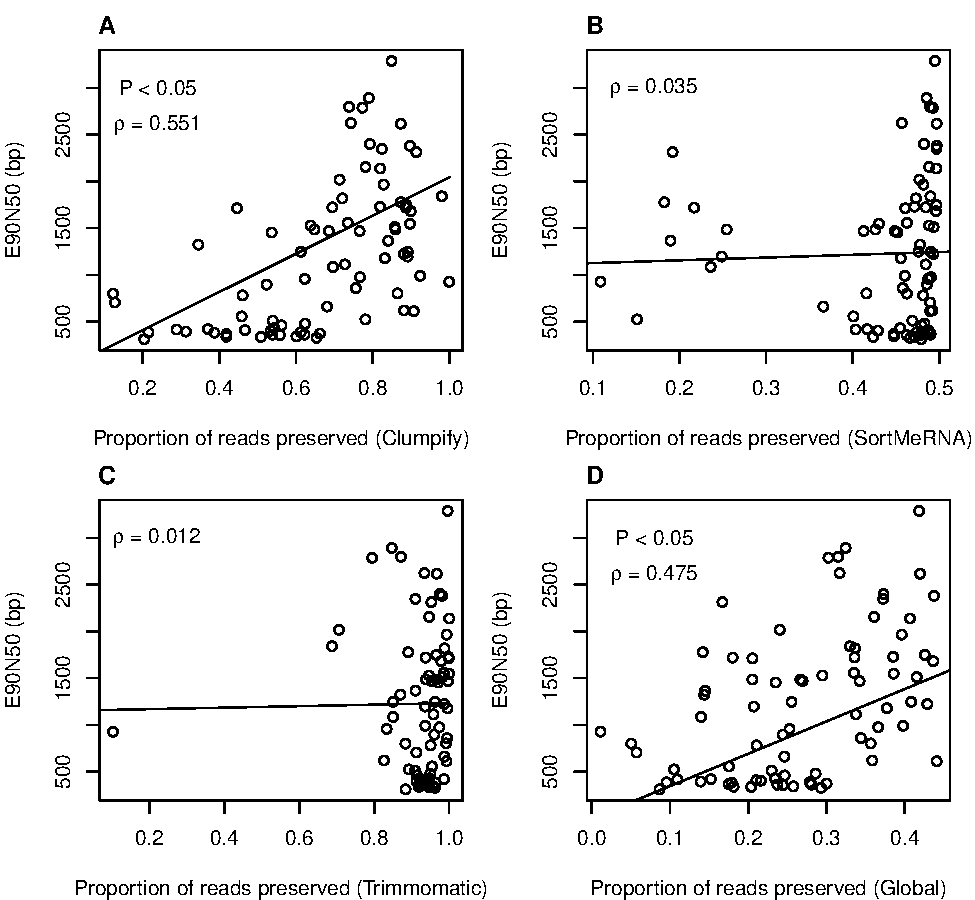
\includegraphics{_main_files/figure-latex/unnamed-chunk-12-1.pdf}

\caption{Effect of the removal of reads after each preprocessing step on the quality of assembled contigs.\label{fig:preprassembly}}
For each program in the preprocessing, the number of reads left in the output was divided by the number of input reads. Programs were used in the order of the pipeline: SortMeRNA operates with Clumpify's output and Trimmomatic with SortMeRNA's. $P < 0.05$ is displayed if the simple linear model with E90N50 (a quality metric for transcriptomic assemblies) as response had a significant regression parameter associated to the proportion of preserved reads. The relationship between variables could be more complex than simple linearity, since best fitting models were not exhaustively explored. $\rho$ indicates the Pearson linear correlation coefficient between both variables. \textbf{A. } Filtering of reads with Clumpify is negatively related to the quality of the assemblies. Furthermore, Clumpify seems to drive the association in \textbf{D.}, which shows that the global filtering of reads in the whole preprocessing has a weaker linear correlation with E90N50 values. Removal of rRNA and COX transcripts (\textbf{B.}) and low quality reads (\textbf{C.}) does not seem to have an effect on E90N50.

\end{figure}

Also, the proportion of reads that are removed by Clumpify seems to have an effect on the outcome of assemblies. The more reads are preserved after the deduplication step with Clumpify in a sample, the higher the E90N50 statistic for that sample (Figure \ref{fig:preprassembly} A). However, there is no evidence to affirm that this is a causal relationship, even if Clumpify operates upstream of Trinity, and the real cause or causes might affect simultaneously all these variables that correlate to each other. Read removal by SortMeRNA and Trimmomatic does not seem to significantly affect the length of the resulting contigs after Trinity (Figure \ref{fig:preprassembly} B, C). Therefore, it is the specific removal of reads by Clumpify that induces this variation in the assembly quality, also because the correlation in Figure \ref{fig:preprassembly} A is higher than in the global reduction of reads (Figure \ref{fig:preprassembly} D). This is surprising, since especially the removal of reads that is achieved with Clumpify, i.e.~deduplication, should preserve one read for each group of equivalent reads. Duplicates do not provide any additional information to the assembly, since there is complete sequence overlap with its equivalent reads and therefore, their exclusion should theoretically not affect neither the length nor the number of assembled contigs.

In all, \(78\%\) of the variation in the reported E90N50 values (\(R^2adj = 0.74\)) could be explained in a linear model with three variables: phylum affiliation, the percentage of reads mapped into contigs and the proportion of preserved reads after Clumpify. All three covariates have significant regression parameters in the model, which indicates that all three are able to provide unique information to reconstruct the distribution of E90N50 values.

\hypertarget{diamond-taxonomic-classification-results}{%
\subsection{DIAMOND taxonomic classification results}\label{diamond-taxonomic-classification-results}}

\hypertarget{description-and-univariate-analysis-of-diversity-1}{%
\subsubsection{Description and univariate analysis of diversity}\label{description-and-univariate-analysis-of-diversity-1}}

Twelve accessions were lost due to errors in the pipeline, probably because the raw sequence files were corrupted, leading to the loss of the only representative in Micrognathozoa phylum, one accession in Brachiopoda, one in Bryozoa, six in Ctenophora, one in Cycliophora and two in Mollusca. In total, 209 observations for 31 phyla remain. Marine (125) and terrestrial (50) habitats are the most prevalent, followed by freshwater habitat with 21 observations. For invertebrates of intertidal zone, 11 viromes have been estimated. Lastly, two observations have been sampled for brackish habitat, both related to mollusks. Again, a significant degree of collinearity is to be expected between phylum and habitat factors (Figure \ref{fig:habitatdivdef}).

\begin{figure}[!htbp]

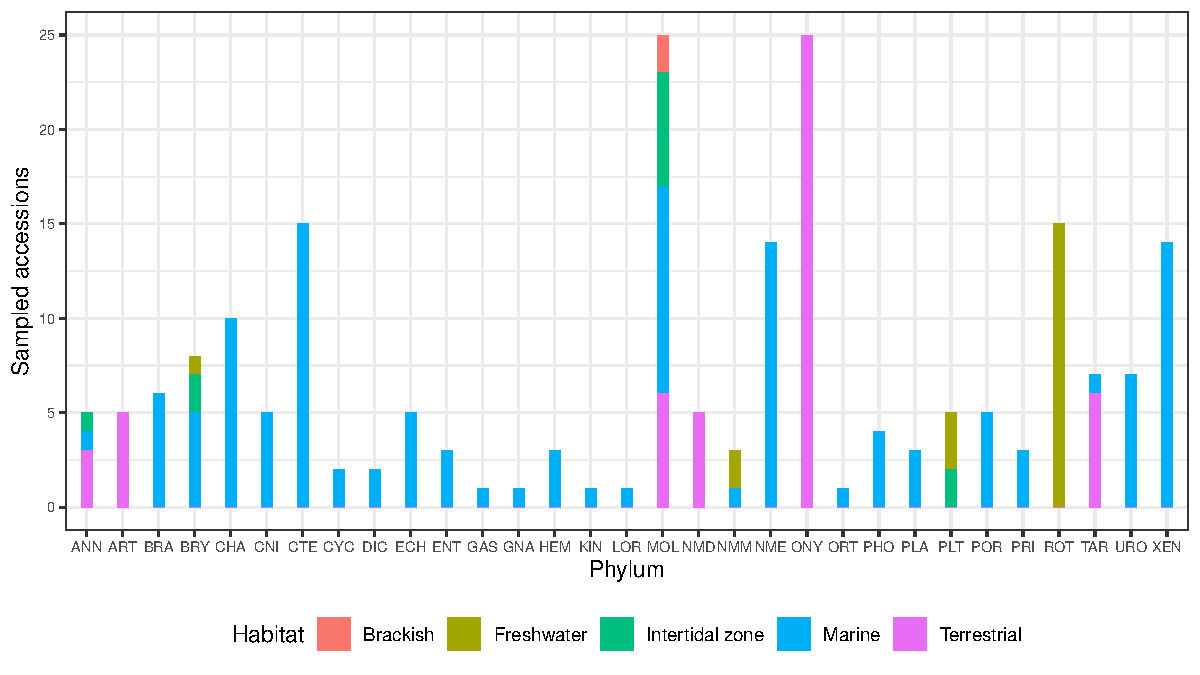
\includegraphics{_main_files/figure-latex/unnamed-chunk-13-1.pdf}

\caption{Distribution of habitats within phyla.\label{fig:habitatdivdef}}
The sampled accessions of 21 out of 31 phyla are exclusively marine. Sampled arthropods, nematodes and onychophores are exclusively terrestrial and Rotifera harbors only freshwater samples. Habitat diversity is only observed within six phyla, with annelids, bryozoans and mollusks being the phyla with greater habitat variability. The unbalance in the exploration depth of the different phyla is also noticeable in the figure.


\end{figure}

After taxonomic classification of contigs, 124 different viral families were found at least once. Non-null virome compositions were reported for all processed accessions and in average \(12\%\) of total non-rRNA, non-COX transcript expression was classified as viral. Between \(6\%\) and \(18\%\) of viral transcripts were found for more than \(50\%\) of accessions, always with respect to the defined subset of the transcriptome. In the pilot test, DIAMOND analysis found approximately \(0.1\%\) of viral transcripts over the whole transcriptome. An increase was expected due to the removal of non-viral sequences in the preprocessing. However, a 120-fold increase cannot be explained just by the exclusion of non-viral reads in the preprocessing, since the total of reads is reduced to about only a fourth of its original size and Clumpify and Trimmomatic are not assumed beforehand to enrich the subsets in viral reads. In other studies, the concentration of viral RNA with respect to the total non-rRNA transcriptome was seen to be more variable and to greatly vary between invertebrate phyla in a range between nearly 0 and almost \(90\%\) \autocite{Shi2016}. The concentration of viral transcripts positively correlates with the E90N50 quality criterion of assemblies (Figure \ref{fig:virqual}) and thus, to the proportion of mapped reads due to their reciprocal correlation. However, \(\alpha\)-diversity does not seem to be affected by E90N50.

\begin{figure}[!htbp]

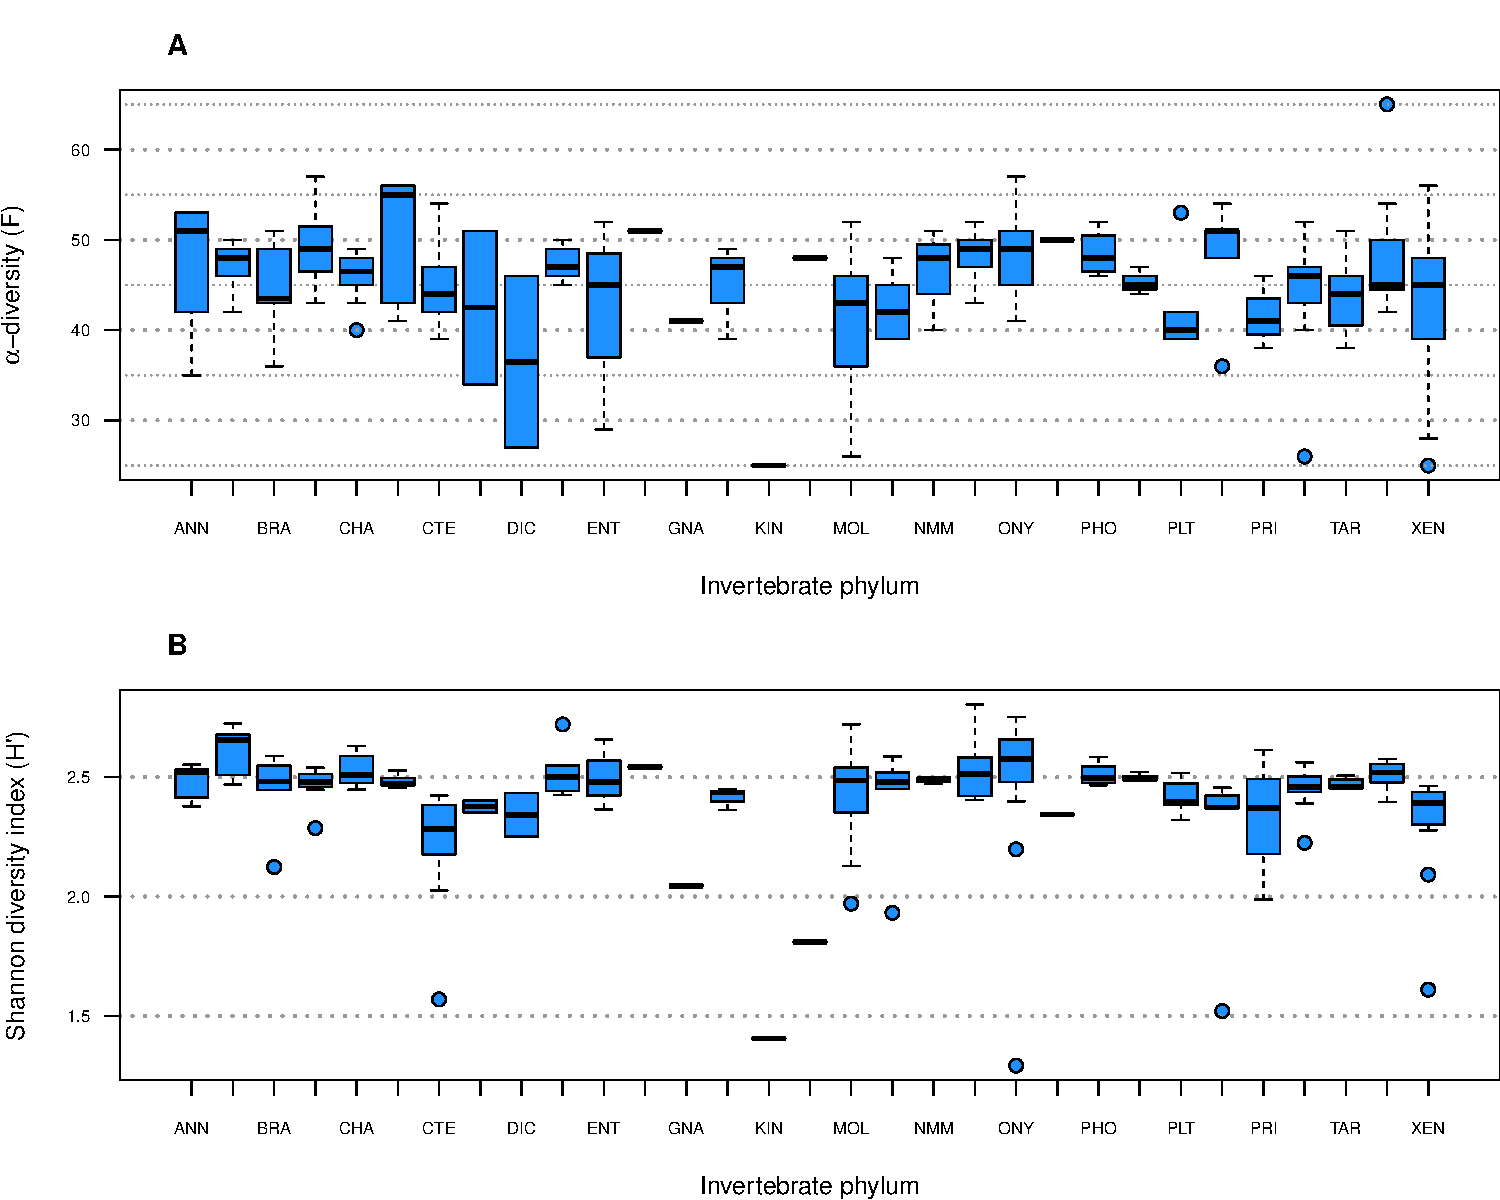
\includegraphics{_main_files/figure-latex/univariate-1.pdf}

\caption{Univariate diversity and abundance metrics for DIAMOND results.\label{fig:defdmnddiver}}
\textbf{A.} Families richness reported per sample across the different phyla in alphabetical order. \textbf{B.} Distribution of Shannon diversity indices per observation in all sampled phyla. The behavior of both metrics is similar. The observed number of distinct families typically ranges between 40 and 55 viral families per invertebrate sample and most Shannon diversity indices oscillate around $2.5$.


\end{figure}

In relation to the identified viral families and their diversity, around 46 viral families were found per sample on average. In all cases, 25 or more viral families were identified for each single observation (Figure \ref{fig:defdmnddiver} A). This is a significant increase in \(\alpha\)-diversity with regards to what was observed both for Kaiju and DIAMOND in the pilot test. Also, \(H^\prime\) values are now higher and oscillate around \(2.5\) (Figure \ref{fig:defdmnddiver} B) in contrast to the values between \(1.5\) and 2 that were seen in the pilot test. Therefore, sufficient evenness has to continue to exist between the abundances of families to achieve an increase in \(H^\prime\) through the identification of more viral families. In summary, it seems that the viral sequences that are found with this combination of programs are more abundant and diverse.

As for the individual viral families, those with the highest relative abundances are predominantly families of dsDNA viruses. In average, transcripts of family \emph{Mimiviridae} represent \(20.1\%\) of the viromes. Other highly abundant families include \emph{Siphoviridae} (\(15.0\%\)), \emph{Myoviridae} (\(7.7\%\)), \emph{Phycodnaviridae} (\(5.2%
\)), \emph{Poxviridae} (\(4.8\%\)), \emph{Baculoviridae} (\(3.0\%\)), etc. Retroviruses represent \(4.1\%\) of viral RNA and the most abundant RNA viral families found are \emph{Flaviviridae} and \emph{Reoviridae}, with average relative abundances of \(1.5\%\) and \(0.8\%\), respectively. \(18.9\%\) of estimated viral transcripts belong to viruses of uncertain family. Again, the viromes associated with the invertebrate samples are dominated by viruses of protists (\(>30\%\)) and bacteria (\(>27\%\)). As many as 54 viral families were found in \(20\%\) or more of the accessions and 15 of them (apart from unclassified viruses) are found in all samples, including most of the above mentioned families.

\hypertarget{virome-composition-analysis}{%
\subsubsection{Virome composition analysis}\label{virome-composition-analysis}}

In this section, phyla with less than five observations were excluded, since within-group variation is not well enough explored in these groups. Still, the distribution of the remaining 181 observations among the 18 phyla left is fairly unequal. First, a dimensionality reduction in the features, i.e.~the viral families, was performed based on their frequency of zero values: those 70 families with \(80\%\) or more null cells along the compositions were excluded.

Like in the pilot test, a selection of PERMANOVA models based on the minimization of AIC was performed using the Aitchison distances. Again, the model with the greatest goodness of fit was the model that included phylum grouping (\(AIC = 2057.1\)) and the addition of the habitat factor as an additive (\(AIC = 2058.5\)) or multiplicative (\(AIC = 2062.9\)) term showed no significant association with differences in location or dispersion that weren't already explained by phylum. In a one-way PERMANOVA model, habitat factor (\(AIC = 2071.8\)) supported rejection of \(H_0\) and was able to explain almost \(7\%\) of the variance in the 181 observations with only five categories. The more informative one-way model using phylum factor was able to explain up to \(26\%\) of the total variance, similar to what was reported in the pilot test (\ref{permapilot}).

In PERMDISP testing, the hypothesis that within-group dispersions are homogeneous (\(H_0\)) for the model with phylum factor was rejected at \(\alpha = 0.05\). In post-hoc Tukey test, Xenacoelomorpha was the phylum with the larger distances to its centroid, while chaetognaths had the most consistently similar viromes (\ref{fig:boxplotdisp}). Xenacoelomorphs are formed by three distinct clades that were historically not related under the same phylum: acoels, nematomorphs and xenoturbellids. Recent phylogenetic studies have led to their union under the same phylum, although they have important morphological differences \autocite{Cannon2016}. This could explain why the compositions of their viromes are so variable, even if they all share the same marine habitat. Chaetognatha is also a phylum of exclusively marine organisms. However, chaetognaths are predominantly found in the zooplankton of warm coastal waters, which poses a restriction with respect to the vast marine habitat.

In contrast, zooplankton species of Ctenophora phylum are notably abundant in a wide range of oceanic habitats. Alongside their phylogenetic diversity \autocite{Christianson2022}, this could be the cause of the greater variation of their viromes. Also, viromes of mollusks were approximately as diverse as in ctenophores. Mollusks are greatly diverse in our categorization of phyla, which could certainly lead to the association to different microbiomes and viromes in each of these habitats. The viral diversity in arthropods is most likely underestimated, since all five sampled species belong to the same class (Arachnida). Apparently, assembly quality is not associated with an increase nor a decrease in virome variability, since Onychophora and Mollusca, which are deeply sampled phyla rich in accessions with low E90N50, do not have a particularly similar nor outlying behavior.

\begin{figure}[!htbp]

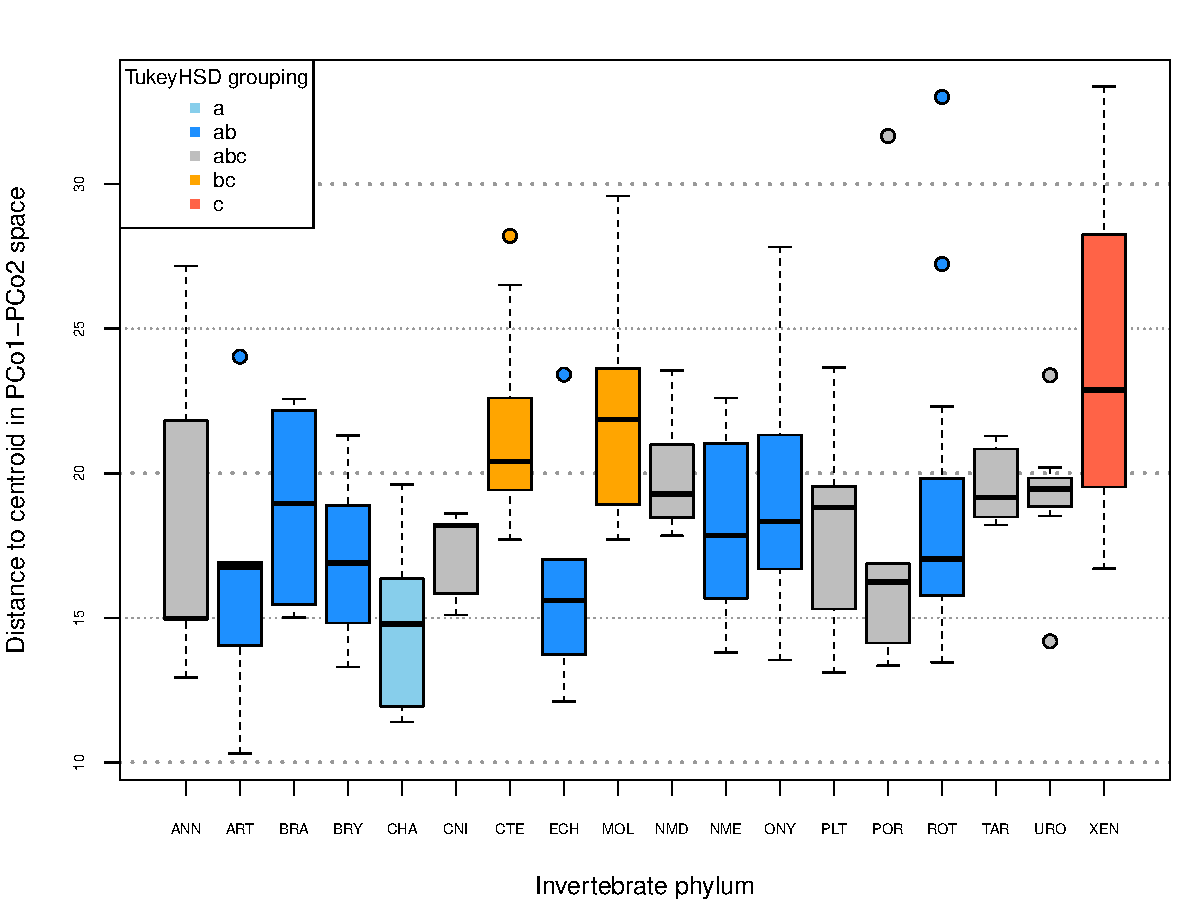
\includegraphics{_main_files/figure-latex/unnamed-chunk-15-1.pdf}

\caption{Distribution of the distances to the centroid in each phylum in the space of PCo1 and PCo2.\label{fig:boxplotdisp}}
Groups of phyla by dispersion were determined with the \emph{post hoc} Tukey test over the PERMDISP model with phylum factor. When the $95\%$ confidence interval for the difference of the mean distances to the centroid between two phyla excludes 0, then those phyla belong to separate groups. This is computed for all pairwise combinations of phyla. Uncertainty in phyla with low sample size does not allow to establish significant differences to other groups, placing them in the ambigous group 'abc', where no differences are found to any phylum.

\end{figure}

PERMDISP analysis using the habitat factor over this dataset showed no significant differences in the variation of viromes between habitats. Here, the inclusion of a category with only two individuals (Brackish) required the test to be more conservative in the rejection of \(H_0\) because of the insufficient exploration of the dispersion in that particular group. Based on the results in both tests, it can be assumed that any differences between the viromes of the different habitats exist and their within-group variations are homogeneous. After PCoA, the representation of all observations in the space of PCo1 and PCo2 shows an intuitive layout of the habitat centroids: viromes of intertidal zone invertebrates share characteristics with terrestrial and marine viromes, while brackish viromes are more similar to marine and freshwater viromes (\ref{fig:habpcoa}). This is coherent with the definition of these two transition habitats. On average, freshwater viromes are the most dissimilar from the rest, which could be an artifact due to the high relative frequency of Rotifera phylum observations, although three additional phyla have this habitat assigned. However, the degree of overlap between the data range of each group is very notable.

Moving back to the phylum grouping, it has been seen that dispersions most likely are heterogeneous among groups. However, it has not been shown whether or not locations differ. This time, PCA results were represented in a figure where centroids per phylum for PC1 and PC2 were drawn (Figure \ref{fig:dmndbiplot}). In order to illustrate the variability of each group in this bidimensional space, \(95\%\) confidence interval ellipses were computed from the covariance matrix for PC1 and PC2 restricted to each phylum. Even if observations are not represented, the resulting biplot-derived figure is considerably dense. Nevertheless, the outstanding virome composition variability of xenacoelomorphs and mollusks can be appreciated in their confidence interval ellipses. As to the locations, most ellipses show overlap with the rest.

For its low variation in PC2, viromes of arthropods appear to be significantly different to viromes of rotifers, tardigrades, nematodes, ctenophores, platyhelminths, sponges (Porifera) and bryozoans. For the same reason, nematodes are separate to onychophores, echinoderms and arthropods, whose centroids are located very nearly. Anyway, nematodes as well as arthopods have small sample sizes, and their variations in PC2 could be underestimated. In the pilot test, viromes of the sampled nematodes and arthropods seemed to be not so divergent (Figures \ref{fig:sample50pcoakaiju} and \ref{fig:sample50pcacat}). Also, it seems that the position of terrestrial observations in Figure \ref{fig:habpcoa} is biased towards the cluster formed by onychophores and arthropods, while tardigrades and nematodes tend to fall between the regions that were considered marine and freshwater. This is likely to be caused by the large number of species analyzed for onychopohores (Figure \ref{fig:habitatdivdef}).

PC3 explained \(7.5\%\) of the variation, which is quantitatively similar to PC1 and PC2. This is indicative of low collinearity between the behavior of the different viral families. Its representation against PC1 or PC2 did not improve the resolution in the segregation of phyla.

As for the contribution of the different viral families to PC1 and PC2, the majority of the most influential families were not identified as such in the pilot test. A high concentration of \emph{Pseudoviridae}, \emph{Adintoviridae} and \emph{Caulimoviridae} transcripts contributes to positive values in PC1. None of these families have confirmed members that infect ctenophores or xenacoelomorphs, which have the most positive values in PC1, but pseudoviruses are known to infect both fungi and invertebrates and adintoviruses have been found associated to cnidarians \autocite{Starrett2021}. Caulimoviruses and especially, potyviruses, which also has a positive effect on PC2, are viruses of plants that also favor positive locations on PC1. As an hypothesis, potyviruses could be found in the phytoplankton associated with the individuals of Xenacoelomorpha and Ctenophora phyla. However, current evidence supports that potyviruses are mainly related to terrestrial plants and insect vectors and their presence in marine habitats is residual if any \autocite{Culley2003,Gibbs2008}.

Mitoviruses (mitochondria and bacteria serve as host), apart from potyviruses, positively contribute to PC2, while many other families are negatively related to this dimension: \emph{Adenoviridae} (animals), \emph{Caulimoviridae} (plants), \emph{Nimaviridae} (marine arthropods), \emph{Virgaviridae} (plants), \emph{Chrysoviridae} (fungi), \emph{Malacoherpesviridae} (mollusks), \emph{Adintoviridae} (invertebrates), \emph{Salasmaviridae} (bacteria), etc. This group of viruses is very diverse in host range. With respect to genome structure, mitoviruses and potyviruses have RNA-based genomes, while among the families that contribute negatively to PC2 only \emph{Virgaviridae} and \emph{Chrysoviridae} belong to RNA classes of viruses. This coordinate opposes tardigrades and nematodes to onychophores, arthropods and echinoderms, whose viromes are enriched in the viral families associated with negative values of PC2.

Rotifera is consistently the phylum found in more negative values of PC1. From the most influential loading vectors, it can be inferred that transcripts of family \emph{Bicaudaviridae} are especially abundant in this phylum, while the contrary occurs with \emph{Pseudoviridae} sequences. Bicaudaviruses are found in hyperthermophilic archaea and, while it is unlikely that rotifers have been sampled from these environments, other related viruses of archaea could have been detected.

In general, the absence of the most overall abundant viral families is notable in the families that influence the PCA the most. Apparently, those abundant families do not introduce sufficient compositional variation between observations and are found in relatively consistent concentrations in the viromes of all phyla and habitats. Therefore, the most abundant families on average, can also be considered the most stable and ubiquitous. However, the minor viral families are able to cause the mild separation of observations in the PCA.

\begin{figure}[!htbp]

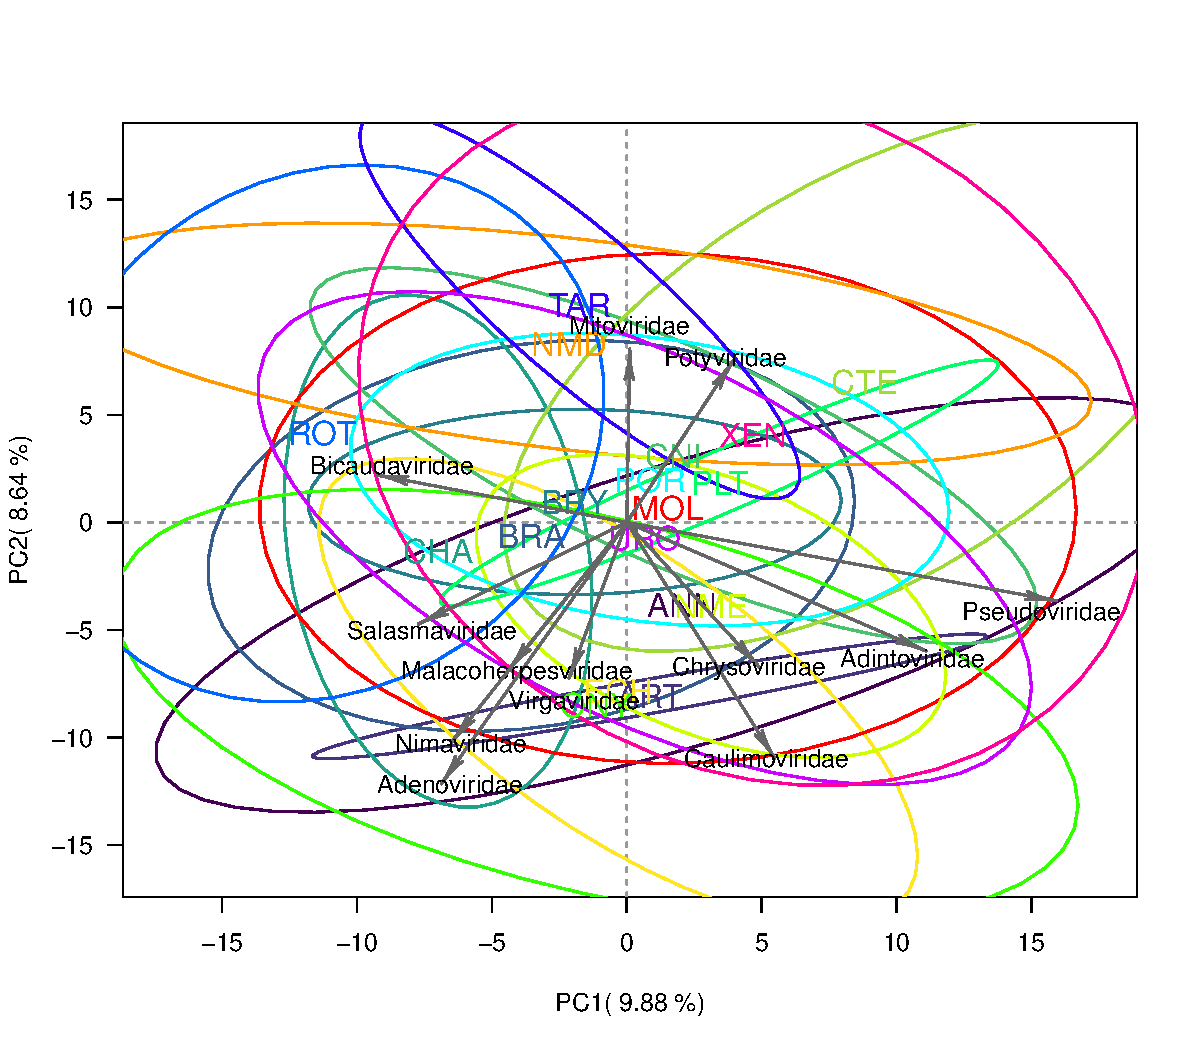
\includegraphics{_main_files/figure-latex/unnamed-chunk-16-1.pdf}

\caption{PCA biplot of DIAMOND results.\label{fig:dmndbiplot}}
Phylum labels are located in their respective centroids in the first two PC. Ellipses for bidimensional $95\%$ confidence intervals were computed with function \texttt{ellipse} of package \texttt{car} using the distribution function of $\chi^2_2$ at $0.95$ as radius and the covariance matrix in PC1 and PC2 as shape. In contrast to the pilot test, where the first two PC could explain at least $30\%$ of the variance in all cases, PC1 and PC2 are here only able to explain roughly $19\%$ of the variation. Even if only the 54 families with less than $20\%$ zero values were included, these orthogonal coordinates could not summarize a larger proportion of the variance probably because of the higher phylogenetic diversity in the definitive analysis.

\end{figure}

A heatmap was drawn to offer a visualization of both the hierarchical clustering of phyla and viral families and the concentration of the transcripts for each viral family in the aggregate virome of each phylum. In this case, within-group variations are completely overlooked. Overall, the average virome compositions estimated for each phylum are fairly similar. Furthermore, the few clusters with nodes that come after long branches in the dendrogram for the phyla do not necessarily involve clear phylogenetic or ecological similarities: for instance, while close evolutionary relationships seem to exist between Rotifera and Chaetognatha \autocite{Frobius2017}, Nematoda has a closer phylogenetic relationships to many other phyla before than Porifera.

As for the viral families, their hierarchical reordering clearly yields at least two distant clusters. The bigger cluster on the right is formed by the most abundant families, while the cluster on the left harbors more scarce families that tend to appear more frequently as the main contributors of PC1 and PC2 in PCA. Arguably, four also seems as a reasonable number of clusters. However, these clusters are again mainly characterized by their abundance. The cluster with higher average concentration is dominated by DNA viruses and viruses of uncertain family. In the rest of the clusters, the majority of viruses are also DNA viruses.

\begin{figure}[!htbp]

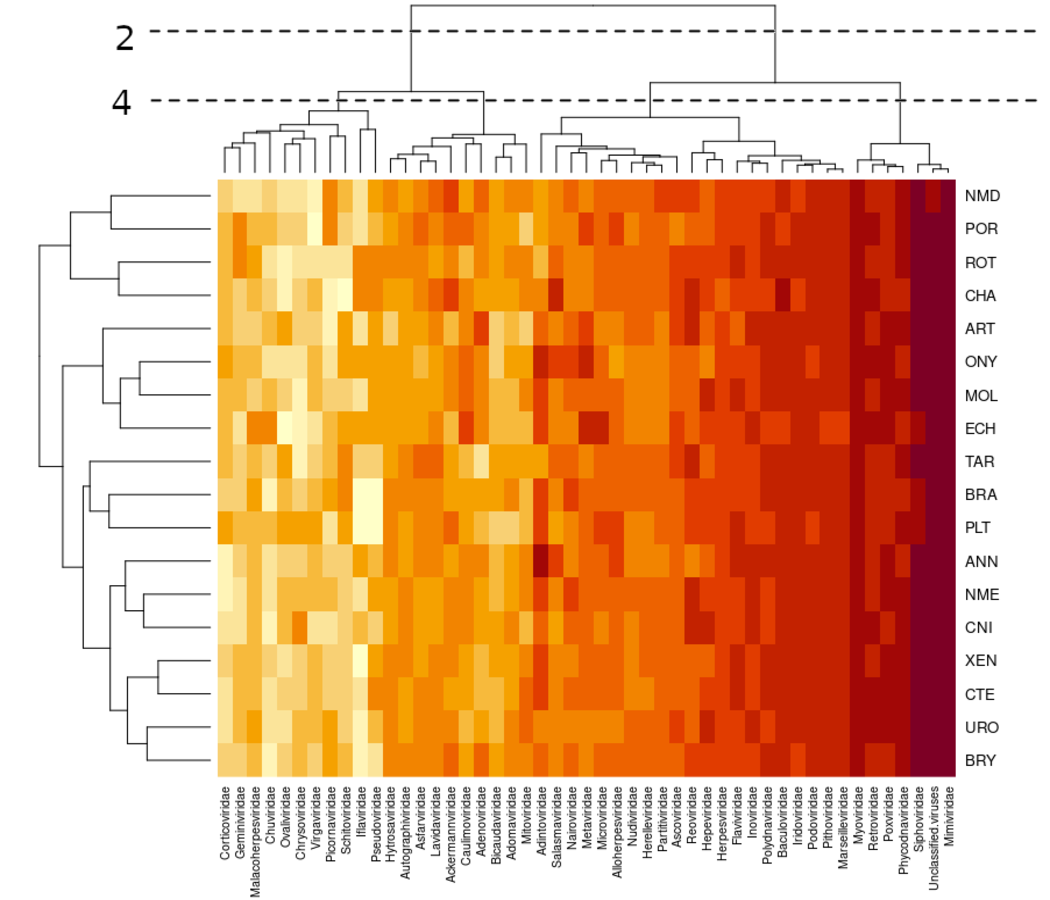
\includegraphics{_main_files/figure-latex/heatmapaggr-1.pdf}

\caption{Heatmap of DIAMOND results.\label{fig:heatmap}}
Compositional vectors of relative abundances were obtained for each phylum after aggregating observations per phylum in the $181\times54$ reduced matrix. Dendrograms were obtained with the complete linkage hierarchical clustering method over the Aitchison distances for rows and columns. Disconitinuous lines indicate two different viral families clustering criteria. High concentration of transcripts is represented with dark colors in the gradient.
\end{figure}

\hypertarget{subset-of-high-quality-assemblies}{%
\subsubsection{Subset of high quality assemblies}\label{subset-of-high-quality-assemblies}}

Since it has been shown that E90N50 in our case influences the relative abundance of viral transcripts within the whole transcriptome (Figure \ref{fig:virqual}) but not the viral families richness, it can be hypothesized that the analysis of high quality assemblies would be able to capture more variation within and between the compositions. The idea behind this supposition is that high quality assemblies involve a higher number of reads mapped to the viral contigs, thus producing more accurate differences to the proportion of expression assigned to each taxon. It was checked that the number of Trinity input reads was not shaping the E90N50 values of the assemblies, so the total number of viral reads is higher in high quality assemblies. Furthermore, longer contigs support a more reliable taxonomic classification based on sequence similarity.

In this case, it was decided to use 1000 bp as the E90N50 threshold to select a subset of high quality assemblies. Among the remaining 129 observations, the observed \(\alpha\)-diversity distribution is not noticeably distinguishable from the distribution observed for the general dataset: the range remains between 25 and 65, the median is identical (46) and the \(IQR\) is just one unit smaller (\(49 - 43\) vs.~\(49 - 42\)). Also, Shannon diversity indices appear to be unaffected by the filtering of accessions with \(E90N50 < 1000\) bp and still hold at values around \(2.5\). Some previously abundant phyla such as Mollusca and Onychophora are reduced to very few observations. Following the procedure conducted for the general analysis, the exclusion of phyla with four or less observations yielded a dataset of 89 observations distributed along 11 phyla (Figure \ref{fig:qualdiver}). Compared to the general analysis, the subset of viral families with \(20\%\) or less zero cells slightly drops from 54 to 52 here. This results in a final \(89 \times 52\) compositional matrix.

As in previous analyses, the one-way PERMANOVA model with phylum as factor yields the lowest AIC among all possible combinations of models with phylum and habitat factors. Both the PERMANOVA and PERMDISP tests with phylum grouping for this dataset suggest the rejection of their respective null hypotheses at \(\alpha = 0.05\). Thus, it can be concluded that dispersions are heterogeneous between phyla, but at this point it is unclear if the rejection of \(H_0\) of PERMANOVA is due to significant differences between the location of centroids and/or just within-group variation differences. The resulting \(R^2\) statistic of PERMANOVA model indicates that \(28.6\%\) of the variance is explained by phylum.

PERMANOVA and PERMDISP contrasts were performed for all pairwise combinations of phyla to further investigate if any locations of the centroids differ and therefore, if any of the estimated virome compositions diverges from the rest. Ignoring the directionality of the contrasts, i.e.~the order in which two groups are expressed, and same phylum comparisons, the number of tests rises to \(\frac{n^2-n}{2}\), with \(n\) being the number of phyla. With 11 phyla, 55 comparisons are made for each test. In order to avoid an increase of type I errors, \(p\)-values were adjusted by the \(FDR\) correction method. Following this methodology, a matrix was constructed to illustrate the significance of the resulting adjusted \(p\)-values for each combination of phyla (Figure \ref{fig:permmatrix}). Again, the virome compositions of xenacoelomorphs and ctenophores appear to be significantly more variable than those of chaetognaths.

A network, or more precisely a graph, was represented to globally illustrate the reported virome similarities and differences for all pairs of phyla (Figure \ref{fig:grafosqual}). In the binarization of the matrix in Figure \ref{fig:permmatrix} used to construct the graph, the following conservative decision was made: viromes of pairs of phyla that resulted in rejection of both PERMANOVA and PERMDISP null hypotheses were considered as not significantly different in location. So, the more connections a phylum has, the more indistinguishable are its viromes from those of other phyla. Brachiopoda and Cnidaria are connected to all phyla, therefore being located in the center of the graph. This shows that their viromes were not found to be any different in composition to those of the rest of phyla. Rotifers are the most eccentric group, showing significant virome composition differences. This was already seen in the general analysis, where it was commented that a possible cause is that the sampled species for this phylum are exclusively freshwater.

Nemerteans, bryozoans and brachiopods, which belong to the superphylum of Spiralia, seem to have a similar profile of connections and thus, are placed nearly in the graph. Rotifers, which also belong to this clade, appear to diverge from the previously mentioned phyla in the graph, probably because those phyla harbor exclusively marine samples. Nematodes and tardigrades, which are both mainly terrestrial and within the Ecdysozoa superphylum, a sister clade to Spiralia, also are closely related in the graph sharing their disconnection to nemerteans. Chaetognatha, Urochordata and Xenacoelomorpha are spread within Bilateria, which also contains the Spiralia and Ecdysozoa superphyla. These three phyla also share the marine habitat, but do not distribute particularly closely and even viromes of urochordates and chaetognaths appear to be significantly different. Lastly, although ctenophores and cnidarians diverged from the rest of animals very distantly, their viromes do not appear to lie especially apart from the rest. This could be explained by their viromes not being as specialized, thus showing similarities to those of the rest of phyla. The phylogeny of invertebrates presented in Dunn et al.~(2014) \autocite{Dunn2014} was taken as a reference. Only clades that result from nodes with broad consensus in the community were mentioned, since the animal tree of life is not completely resolved and is still subject to revision.

It must be taken into account that the number of edges that connect each phylum vertex to others seems to be affected by sample size. Phyla with few observations are placed in the center of the graph, while phyla with more than 10 observations (Figure \ref{fig:qualdiver}) are all located in the periphery. Again, it can be seen that there is uncertainty in the estimation of `average' virome compositions in phyla with low sampling depth. It remains unclear if there is an excess in the rate of false negatives in small phyla or an excess of false positives in larger phyla. In summary, the position and links of a phylum in the graph appear to be shaped by their sampling depth and to a lesser extent by their habitats and their evolutionary relationships to other phyla.

\begin{figure}[!htbp]

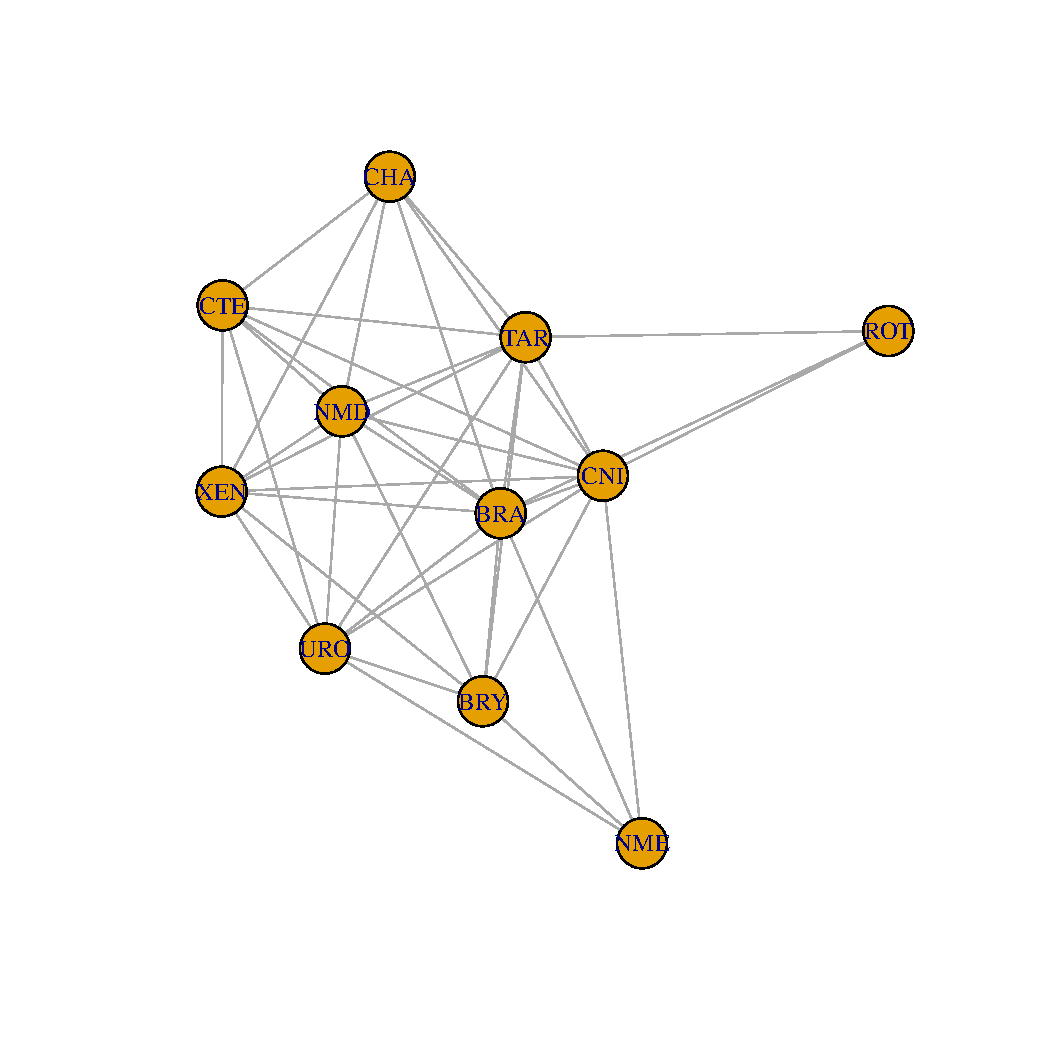
\includegraphics{_main_files/figure-latex/unnamed-chunk-18-1.pdf}

\caption{Virome equivalence network after pairwise PERMANOVA.\label{fig:grafosqual}}

An adjacency matrix was constructed after converting the $p$-value significance matrix for all combinations of phyla to a binary matrix, where 0 represents only differences in location (significant rejection of PERMANOVA $H_0$) and 1 the rest of possibilities. In the graph, this involves the connection (1) or the separation of vertices (0). Self phylum connections are omitted in this unweighted, undirected graph. The result is a figure that allows the simultaneous visualization of the distinctness or similarity between the viromes of all pairs of phyla. In short, edges represent the equivalence of the 'average' viromes of the vertices they connect.

\end{figure}

The number of observations has halved with regards to the general analysis and the representation of a biplot with all scores is not as saturated here (Figure \ref{fig:pcaqual}). An increase up to \(23.3\%\) is noted in the total variation explained together by PC1 (\(13.7\%\)) and PC2 (\(9.6\%\)). Since this is just the analysis of a subset, it was expected that the viral families that are able to summarize a higher proportion of variation in the first two PCs would be essentially the same as in the general analysis, even if some phyla and observations with low quality assemblies were excluded. All viral families displayed in the biplot, i.e.~the most influential in the separation of virome compositions, are found within the 58th percentile of families with the lowest assigned mean concentration and the 69th percentile of maximum concentration by family. In short, the RNA molecules of these families are scarce, but variable between observations. However, this is not an artifact due to the procedure of zero replacement, since the observed tpm values for these families are not below the established tpm detection limit (\(0.01\)). As for the scores, every phylum has its observations relatively grouped and the heterogeneity of dispersions can also be appreciated between the previously mentioned phyla. With respect to habitats, whose information was omitted in the graph, marine, freshwater and intertidal bryozoans are more or less grouped in the central-low region of the biplot, suggesting that phylum has a larger role in the profiling of these viromes. This is homologous to what can be observed in the case of Tardigrada, where its only marine observation is located within the range of its observed terrestrial individuals.

\hypertarget{discussion}{%
\section{Discussion}\label{discussion}}

In the first place, the introduced preprocessing steps and the reduction of the reference database used by DIAMOND made it possible to analyze a higher number of accessions in a shorter time. However, the presented definitive analysis still covers a limited part of the available datasets. In most phyla, one accession of each of their species was sampled and processed. The confidence in the estimation of virome variability and proper composition in scarcely sampled phyla hinders the applicability of the presented statistical methods on them. The interest in these phyla might not rely so much on the comparison, but on the presence-absence or abundance profiles of their individual compositions, which is not the aim of this study.

The removal of reads by each of the preprocessing steps is variable among observations, but deduplication generates the largest variability in the proportion of discarded reads (Figure \ref{fig:preprocess}). Exact duplicates not only happen due to experimental reasons, but also due to biological ones and both of these sources of variability exist in the data. Biologically meaningful duplicates can be found in sufficiently abundant transcripts, since the probability of obtaining two or more exact reads or pairs of reads from these sequences not as an artifact of the sequencing platform is not negligible. In differential gene expression studies with single-end RNA-Seq data, where transcript abundance is taken into account, the application of deduplication methods tends to increase the rate of false negatives, especially for genes of moderate to large abundance \autocite{Klepikova2017}. However, all accessions processed in the definitive analysis possessed paired-end libraries. Another study shows how removal of duplicates in RNA-Seq are detrimental to overall alignment statistics because of the high proportion of reads eliminated, but also improve the detection of biological signal in differential gene expression analyses, while retaining the fold changes in the expression of a single gene \autocite{Dozmorov2015}. In our case, it is of primary interest to investigate if removal of duplicates has an effect on the proportionality between the abundance of transcripts of different genes, OTUs or more precisely, viral families. However, this remains unclear and would imply that some sequences are more prone to duplicate generation than others. Duplicate removal is completely established in the analysis of genomic data, but is still an object of discussion in transcriptomics. In RNA-Seq, deduplication can be performed experimentally by unique molecule labeling, prior to PCR amplification \autocite{Fu2018}, with the purpose to distinguish biological from experimental duplicates.

The proportion of removed rRNA and COX reads with SortMeRNA shows that in most cases, the commonly acknowledged benchmark of \(80\%\) rRNA expression among the whole RNA population has not been achieved. This is probably due to the inclusion of only the sequences of 18S and 28S rRNA but not mitochondrial RNA. The proportion of mitochondrial expression, of which COI, COII and COIII are a part, is very dependent on the sequenced tissue and in mammals is observed in the range of almost 0 to \(30\%\) \autocite{Mercer2011,Osorio2021}. Therefore, the variability of the observed proportion of reads filtered with SortMeRNA probably depends on \emph{(i)} the abundance of mitochondrial RNA found in the sample, which also includes the 16S and 12S rRNA subunits of mitochondrial rRNA, \emph{(ii)} the abundance of microbial RNA, which will probably be associated to a decrease in the rate of read removal, since its rRNA transcripts for the 16S, 5S, and 23S microbial rRNA genes have not been targeted. Then, it can be assumed that the RNA populations in accessions where \(80\%\) of reads were mapped to eukaryotic rRNA and COX sequences were not rich in mitochondrial and/or prokaryotic transcripts.

The nature of the RNA populations sequenced in each sample was resolved with the use of this preprocessing step of ribosome depletion. Since \(50\%\) or more of reads were left out in all cases and COX transcripts are not known to be able to account for this much of expression, rRNA transcripts have to be present in all libraries. Then, neither ribosome depletion nor poly-A selection of mRNA were performed prior to sequencing. This was expected, since this set of accessions was provided by a team of researchers who focused on the phylogenetic study of rRNA. Nevertheless, the lack of standardized metadata regarding this question in the SRA database and the large number of accessions made it reasonable to doubt if all accessions were homogeneous in this sense.

It appears that the order of the steps in the preprocessing does not have an effect on the proportion of reads filtered by each one, since no strong correlation has been found between any pair of proportions of kept reads. Therefore, in terms of speed, it would seem appropriate to place SortMeRNA in the last place, since it shows the longest runtimes.

With regards to the proportion of mapped reads, which has a very important effect on E90N50 (Figure \ref{fig:assemblystats} B), the variability observed among samples might respond to a broad series of reasons. Once filtered by quality, all fragments of a sufficiently sequenced transcript should, in theory, be able to reconstruct the sequence of a contig. An exception can occur when a transcript is rich in low complexity regions, which can cause ambiguity in the alignment and mapping of reads \autocite{Rado-Trilla2012}. It is unknown if the occurrence of this phenomenon is likely to differ between different groups of invertebrates as it is difficult to identify sources of variation for the transcriptomes of invertebrates as a whole, given the limited availability of molecular knowledge for some phyla. Variable sequencing depth can also induce differences in the proportion of mapped reads and the quality of assemblies, especially in the context of transcripts of rare occurrence. An insufficient sequencing depth involves the partial or null reconstruction of contigs, which leaves reads that biologically stem from the same transcript as unrelated. However, this appears not to be the case here after processing only accessions with more than 3 Gb sequenced, since library size shows no relation to both of these assembly statistics.

The E90N50 qualities of the assembled transcriptomes appear to be independent from the proportion of reads filtered with SortMeRNA and Trimmomatic (Figure \ref{fig:preprassembly} B, C). However, libraries that undergo a more intensive reduction of reads at Clumpify tend to form assemblies of lower quality that are able to map a lower proportion of reads (Figure \ref{fig:preprassembly} A). As it affects both E90N50 and the percentage of mapped reads similarly, this removal of reads does not seem to selectively target reads of particular transcripts, which would reduce the proportion of mapped reads but not the E90N50, except if precisely the longer transcripts were targeted. Instead, it seems that reads are lost indiscriminately, which causes shorter contigs to occur. This seems problematic and deserves further investigation, since the negative effect of deduplication on the quality of assemblies has not been previously reported to our knowledge.

Another aspect that remains unclear is the positive relationship between the values of E90N50 and the relative abundance of viral transcripts as classified with DIAMOND. This implies that for transcriptomes whose set of \(90\%\) most abundant transcripts are formed by longer contigs, a higher proportion of viral transcripts is found. From another point of view, the longer the contigs are that cover \(90\%\) of expression, the more scarcely will the host transcripts be found within the transcriptome. Many hypotheses can be speculated that could simultaneously contribute to explain this scenario.

For instance, transcriptomes dominated by shorter contigs could have a high presence of prokaryotic rRNA, which can account for an important part of the total expression, thus reducing the relative abundance of viral RNA. Another possible cause could be that transcripts of viruses, or at least the most abundant ones, are longer than those of its host. This seems counter-intuitive given that it is often acknowledged that viruses tend to shorten its genome and proteins \autocite{Belshaw2008,Rappoport2012}, but it is worthy to note that apparently giant DNA viruses dominate these viromes and may involve other evolutionary strategies. Genomic RNA molecules of viruses could be longer than the average host transcript, although such an important effect from these molecules could be unexpected given the overall low abundance of RNA viruses.

An important aspect of the effect of assembly quality on the estimated viromes is that the number of different families identified for a particular sample is constant for the range of observed E90N50 values. Then, although assemblies of higher quality assign a higher proportion of expression to viruses, the underlying viral \(\alpha\)-diversity at the level of families has already been identified. Similarly, Shannon diversity indices, which additionally take into account the evenness among viral families, also seem constant on the observed range of E90N50. Therefore, it seems that diversity is not affected by assembly quality in the range of 500 to 3000 bp, even if one may think that a higher rate of false negatives should occur in assemblies made up of shorter contigs or with a lower proportion of mapped reads. The effect of E90N50 on the relative abundance of viruses but not on their diversity does not seem to translate into an effect on the estimated compositions of viromes, since phyla with more compositional variation are not necessarily rich in low quality assemblies. Since evenness and compositions were not significantly affected by assembly quality, it can be assumed that the increase in the relative abundance of the global virome along with E90N50 maintains the proportionality between the virome components. In summary, low E90N50 did not produce significant detrimental effects on the analysis of compositions, although longer contigs are always prefered for alignment-based analyses, such as taxonomic classification.

As for the identified viral families throughout the pilot test and the definitive analysis, it seems that invertebrates are in very tight contact with their microbiomes and the viromes they harbor. This is suggested by the high abundance of transcripts taxonomically annotated to families of bacteriophages and viruses of protists. However, it must be noted that a sequence of a yet unknown virus could be classified to a closely related family with a different host range to that of the novel virus. For example, viruses related to giant DNA viruses of protists have been found infecting chaetognaths, although no genomic information of it is yet available \autocite{Shinn2018}. If sequence divergence was not too clear, a transcript of one of these viruses could be classified to a family with a misleading host range. Additionally, the recognised host range of a viral family does not necessarily summarize the complete range of hosts that all known and unknown viruses of that family can infect. In recent years, a number of interkingdom events of horizontal virus transfer have been found \autocite{Liu2016,Nerva2017}. For example, the first identification of a partitivirus that is able to infect and replicate in invertebrates \autocite{Cross2020} has broadened the host range of this family, formerly acknowledged to infect fungi, plants and protists.

Furthermore, identified viral sequences do not necessarily involve the true presence of those viruses in the sample, since the identified transcripts could result from EVEs and all types of genome integration of viral sequences into transcriptionally active genome regions. In this case, the identified viral sequence arises from a past contact between the virus and its invertebrate or microbial host, but not at the moment of infection. The importance of EVEs in invertebrate genomes has recently been acknowledged, especially in arthropods \autocite{Flynn2019}. In ants, the abundance of relatively ancient and recent EVEs of very diverse RNA and DNA viruses allows for the reconstruction of ant phylogenies and suggests the presence of functional proteins of viral origin in the ant genome \autocite{TerHorst2019}. Additionally, some of the identified EVEs in this study are closely related to families reportedly unable to infect invertebrates, but that are found in the diet of invertebrates, e.g.~totivirus and chrysovirus-related EVEs have been found in the genomes of fungus-growing ants. It is unknown to which extent this can be generalized to some or all invertebrate phyla, but EVEs are likely to play an important role on the estimated viromes.

One of the main results of the definitive analysis is that virome diversity is relatively stable among all studied invertebrate phyla: approximately the same number of different viral families were found for all samples. This is consistent with the findings in the pilot test, since the effect of insufficient library sizes was practically eliminated after filtering out accessions with less than 3 Gb sequenced. Consequently, viromes of marine invertebrates are not particularly more or less rich than viromes of terrestrial invertebrates, as viromes of sponges are not more or less complex than viromes of more recent invertebrate phyla, for example. In Zhang et al.~(2021) \autocite{Zhang2021}, \(\alpha\)-diversity of marine invertebrate viromes appeared to be more variable within phyla than between phyla. This contrasts with the more pronounced virome composition differences that are found between vertebrates and invertebrates \autocite{Mahar2020}. The present results suggest that the differentiation between viromes of more phylogenetically distant phyla of invertebrates is milder than between vertebrates and invertebrates, although it would be advisable to include vertebrate transcriptomes in the analysis in order to confirm this.

Abundance and virome composition of RNA viruses was already reported to be notably variable within phyla and not very divergent between phyla in basal and apical positions of the tree of metazoans \autocite{Shi2016}. Similar conclusions were found in a transcriptomics study of the DNA viromes associated with invertebrates of several phyla, where a notable abundance of bacteriophages and viruses of protozoans was found \autocite{Porter2019}. However, some of the most prevalent viral families in this study were \emph{Genomoviridae}, \emph{Circoviridae}, \emph{Parvoviridae}, which are known to carry species that are able to infect invertebrates. These families were identified at least once in the definitive analysis, but their transcripts were nowhere as abundant as those other families, such as \emph{Mimiviridae}. The most abundant families of viruses that are likely to infect invertebrates, after ignoring bacteriophages and viruses of protists, are poxviruses (\(4.77\%\) of viral RNA), retroviruses (\(4.12\%\)), baculoviruses (\(3.04\%\)), iridoviruses (\(1.93\%\)), polydnaviruses (\(1.64\%\)), flaviviruses (\(1.48\%\)), adintoviruses (\(0.98\%\)), herpesviruses (\(0.87\%\)), reoviruses (\(0.78\%\)), hepeviruses (\(0.72\%\)), metaviruses (\(0.58\%\)), nairoviruses (\(0.40\%\)) and ascoviruses (\(0.40\%\)). This constitutes a very diverse group of DNA, RNA and retro-transcribing viruses, although the most abundantly found families have DNA-based genomes. The host range of some of these apparently ubiquitously abundant families, such as \emph{Poxviridae}, \emph{Herpesviridae} or \emph{Hepeviridae}, include humans and other vertebrates. However, it remains unknown if the identified viruses for these families pose a real risk of vertebrate infection.

Viromes of invertebrates are commonly acknowledged to be characterized by a large abundance and diversity of RNA viruses, rather than DNA viruses \autocite{Harvey2022,Porter2019}. However, RNA originating from DNA viruses appeared to dominate the population of viral RNA both in the results of the pilot test and the definitive analysis. DNA viruses tend to have larger genomes than RNA viruses, but it is the level of expression which is being measured in transcriptomics. Furthermore, transcripts and genomes are surveyed in the case of RNA viruses. So, levels of expression in DNA viruses for the analyzed datasets have to be generally higher than those of RNA viruses. It is unknown if any or some of the transcriptomics datasets included a selection step or methodology that selectively affected RNA viruses with respect to DNA viruses, although it seems unlikely given that their initial purpose was not that of virus analysis.

In a metagenomics study on the DNA viromes of four different marine invertebrate phyla (Arthropoda, Cnidaria, Echinodermata, Urochordata), bacteriophages of families \emph{Myoviridae}, \emph{Podoviridae} and \emph{Siphoviridae} were found to be undoubtedly the most abundant and spread viral families in the sampled organisms \autocite{Gudenkauf2016}. Interestingly, protist viruses of \emph{Phycodnaviridae} were also found in a very remarkable overall abundance. However, \emph{Mimiviridae}-related sequences were not reported to dominate the viromes nowhere as much as in the presented results. Although the use of DNA or RNA data as a source to measure viral abundance has important differences, one possible explanation for this fact might lie in the changes that the nr database, which is also used in this study, can have suffered over the last six years.

The exceptional abundance of mimiviruses and siphoviruses in our results could be either due to \emph{(i)} a true ubiquitous presence of these and/or closely related viruses, \emph{(ii)} the integration of EVEs related to these families in transcriptionally active regions or \emph{(iii)} the opposite situation, i.e.~the integration of host genes in the genomes of these viruses. In this case, the hijacked gene would have to be annotated in the reference database as belonging to that virus species. Then, even if this chimeric virus was absent from a sample, the presence of a sufficiently similar transcript of the original microbial or invertebrate host gene would be detected as a viral sequence. This is an important shortcoming of the presented taxonomic classification, since the fact that a contig could be more similar to an eukaryotic or prokaryotic sequence than to a viral sequence was ignored. Instead, every contig with a viral hit with an E-value lower than \(1e-05\) was considered viral. This was made in order to improve sensitivity, since ignoring all contigs with a more similar eukaryotic hit could eliminate true viral sequences for their similarity to an EVE. Even if this occurred, it must be a host gene that is very abundantly expressed.

Additionally, it has been shown how these highly abundant viral families were not able to profile the differences between the viromes of invertebrates of different phyla. Instead, infrequent viral families generate the compositional variation between the observations. The relative information in the parts of a composition, whose values are very low or near to the detection limit, might be more sensitive to the noise, i.e.~false negative and false positive rates. For instance, the relative contribution to the whole for a family with one read mapped is doubled when one further read is classified to it. This is avoided to a certain extent by the selection of a subset of viral families prior to compositional analysis. However, there is no universally accepted criterion for the dimensionality reduction of features in the compositional analysis of microbiomes or viromes. In this study, criteria based on sparsity in the compositional matrix and the maximum observed relative abundance were used. In Xia et al.~(2018) \autocite{Xia2018b}, parts have to met the requirement of having a minimum relative abundance higher than \(0.1\%\) in order to be kept for the analysis. One could think of other methods, using other location measures such as the mean or introducing the variability in each part. In all cases, it involves the establishment of an arbitrary acceptance-rejection threshold. The use of a different dimensionality reduction criterion could have had an important effect on the rare viral families that were able to generate more variability between observations.

It has been shown in both the pilot test and the definitive analysis that phylum is able to explain approximately 21 to 30\(\%\) of the virome differences between invertebrate samples (28 to 30\(\%\) for compositions generated with taxonomic classification of contigs with DIAMOND). Phylum segregation of samples was significantly associated with differences in the virome compositions in all tested datasets. Habitat factor was also significantly associated with virome differences, although the amount of variance explained by phylum grouping was always superior (one-way habitat models generally explained less than \(10\%\) of the variance). Furthermore, it has been shown that the additive or multiplicative inclusion of habitat factor in a PERMANOVA model with phylum factor does not achieve a better goodness of fit than the one-way model with just phylum grouping. Therefore, the habitat factor did not provide important information with respect to virome compositions that was not already covered by the phylum factor. However, collinearity between phylum and habitat factors reached a very high degree in the analyzed datasets, which can lead to this situation. Therefore, these results do not suggest that the habitat of the invertebrates does not have an effect shaping the composition of its virome. Ideally, this would require the sampling of invertebrates of variable habitats within fixed phyla, while trying to achieve a balance between the sample sizes of habitats, if possible.

The evolutionary history of invertebrate viruses is thought to involve a long history of host-virus co-divergence and numerous horizontal virus transfers with other invertebrates and more distant organisms \autocite{Harvey2022}. The former could be approximated with the phylum factor, while the latter could be related with the habitat of the invertebrate, which influences the pool of organisms from which viruses can be transmitted, e.g.~plants in terrestrial environments. Then, viromes of closely related phyla would be expected to be similar, as a consequence of co-divergence, as viromes of closely related habitats, since the invertebrate could be in contact with similar organisms which harbor their own viromes. Co-divergence was not identified between the analyzed phyla, as the observed similarities between the viromes of different phyla do not reconstruct their phylogenetic relationships in the tree of animal life (Figure \ref{fig:grafosqual}). This could have been masked by the presence of other organisms in the samples, especially microbes, but it could be better examined with a more intensive sampling of phyla and balanced sample sizes, if possible. As for the habitats, it has been shown that viromes of marine, terrestrial and freshwater samples (Figures \ref{fig:sample50pcacat} and \ref{fig:pcaqual}) tend to be different. Viromes of freshwater samples, which are represented mainly by platyhelminths and rotifers, are especially divergent from the rest. Transition habitats, such as intertidal zone, which mediates between marine and terrestrial habitats, and brackish water, which is located between marine and freshwater habitats, seem to carry similar viromes to those of their respective related main habitats (Figure \ref{fig:habpcoa}).

Additionally, dispersion of viromes within particular phyla or habitats were increased after deciding to sample only one observation per species. Although some species and their viromes can still be very closely related within a phylum, e.g.~same-genus species, observations seem to be more scattered in the PC1-PC2 or PCo1-PCo2 space than in the analyses of the pilot test using taxonomic classification of contigs (Figure \ref{fig:sample50pcadiamond}). This is necessary in order to not underestimate the variability of the viromes in the different phyla, although the phylogenetic relationships between species were not controlled. For instance, virome exploration in a phylum can be greatly hindered by the analysis of a very narrow range of related species, which is the case for arthropods, from which only arachnids were sampled.

Finally, some remarks about the statistical analysis will be presented. First, an analysis of outliers has not been performed. And even if it does not seem that some individuals in the definitive analysis can constitute outlying observations judging from their distribution in the PCOa or PCA plot, identification of multivariate outliers is not trivial. Multivariate outliers are known to have a great effect on SVD. However, the covariance matrix of \emph{clr}-transformed compositional data is singular, which prevents the use of the classical Mahalanobis distances. To date, the use of other logratio transformations, such as \emph{ilr}, and robust Mahalanobis distances are the preferred multivariate outlier detection method for compositional data \autocite{Filzmoser2012}. Second, although it was avoided to use groups with less than five observations in PERMANOVA and PERMDISP analyses, sample sizes were notably unbalanced. While PERMDISP allows for the adjustment of this kind of bias directly in \texttt{R}, the classical definition of pseudo \(F\)-ratio in PERMANOVA can lead to an inflation of type I error in the presence of unbalanced groups and heterogeneity of dispersions. Several solutions have been proposed to this problem \autocite{Anderson2017b,Alekseyenko2016}, although neither of them is still implemented in package \texttt{vegan}.

\hypertarget{conclusion}{%
\section{Conclusion}\label{conclusion}}

In conclusion, we have presented the whole procedure of a meta-analysis of public invertebrate transcriptomic datasets in the context of whole virome identification. First, the development and selection of an accurate and time-efficient pipeline for the taxonomic classification of sequences into viral families was conducted. The final pipeline included preprocessing steps for the trimming of adapters and the removal of reads based on the occurrence of sequence duplicates, their affinity to eukaryotic rRNA and their sequencing quality. High rates of deduplication were found to be associated with a decrease in the quality of assemblies (E90N50) and the percentage of reads mapped to contigs. However, assemblies of low quality were apparently able to reconstruct the diversity and composition of viromes similarly to high quality assemblies.

Second, the ecological abundance matrices resulting from the application of this pipeline were set to be analyzed under the framework of compositional data analysis. In recent times, these methodologies are gaining popularity in the study of ecological community structures, in contrast to classical methods used in ecology. The application of compositional data analysis procedures is more robust, since it acknowledges the characteristics of communities such as viromes and the goals that researchers tend to have over these types of data. In our case, the application of PERMANOVA and PCA using Aitchison distances and \emph{clr} transformations, i.e.~classical compositional data analysis methods, has been used in order to identify differences in the virome compositions of invertebrates between different phyla and habitats.

To our surprise, we found that viromes were remarkably similar between invertebrate species of very distant phyla. However, phylum classification of invertebrate samples was able to summarize almost \(30\%\) of the total variance between viromes for different datasets. In all occasions, phylum classification has been found to be more informative than habitat with respect to invertebrate virome composition. Although the evolution of invertebrate viruses is thought to be explained by an hybrid history of virus-host co-divergence and numerous events of cross-species virus transmission, this has not been clearly identified for the sampled dataset.

In this meta-analysis, the use of metadata in the SRA database has been of great importance. For instance, invertebrate taxonomy, the amount of sequenced bases and the type of sequencing library metadata were all recovered from this database and used in order to better characterize each sample. These fields are complete for all accessions. However, there are lots of other non-standardized and incomplete fields that could provide very valuable information about the ecological environment of the sample, the experimental conditions and its geographical coordinates. Although metadata regarding the sequencing technology used to generate a dataset are generally available, information about the presence or absence of a step for the selection of a particular RNA molecule population is lacking. It was checked that all sampled datasets did not originate from ribosome-depleted or poly-A-selected transcriptomes after mapping reads to rRNA sequences. This is an important shortcoming of this meta-analysis, since the experimental procedures used in some samples might not be suitable for the analysis of viruses.

It must be noted that the results are entirely dependent on the bioinformatics pipeline and especially on the reference database that is used in the taxonomic classification of sequences. Although it has not been presented for the definitive analysis, viruses found with Kaiju in the pilot test are not radically different for those found with DIAMOND. Overall, the dominance of the same or similar families of DNA viruses is noted. Viromes of invertebrates have always been recognised to harbor a higher diversity of RNA viruses. However, the observed abundance of DNA viruses appears to be partly influenced by the presence of microbes associated with the invertebrate samples.

As a final remark, this holistic approach to the diversity and the abundance profile of virome compositions in invertebrates is likely to ignore the presence of unknown viruses, especially in understudied phyla. Reference databases are in constant development and the identification of novel virus species in bottom-up studies is the basis over which (meta)viromics can be constructed. Furthermore, (meta)viromics studies, such as the present one, commonly require the annotation of each virus to a taxonomic lineage, which involves the consensus of virologists and, sometimes, the rearrangement of entire taxa in order to fit the new discoveries. All in all, the outcome of holistic projects in virology largely depends on the efforts of the entire community of virologists.

\hypertarget{note}{%
\section*{Note}\label{note}}
\addcontentsline{toc}{section}{Note}

This is a reproducible report generated in an \texttt{R} project with Bookdown version 0.24 \autocite{Xie2016,Xie2022}. The data, the code and its package requirements are accessible in \url{https://github.com/palf98/metaviromics}. The code was developed using \texttt{R} version 4.0.4 in RStudio version 1.4.1717.

\hypertarget{supplementary}{%
\chapter{Supplementary}\label{supplementary}}

\begin{table}[!h]

\begin{threeparttable}
\caption{\label{tab:fqd-speed}Comparison of the average download speed of different fastq download programs from SRA accessions.}
\centering
\begin{tabular}[t]{lc}
\toprule
Method & min/GB of compressed fastq file\\
\midrule
\cellcolor{gray!6}{fastq-dump} & \cellcolor{gray!6}{8.97}\\
fasterq-dump (25 threads) + pigz (25 threads) & 1.02\\
\cellcolor{gray!6}{parallel-fastq-dump (--gzip; 25 threads)} & \cellcolor{gray!6}{1.5}\\
parallel-fastq-dump (25 threads) + pigz (25 threads) & 1.77\\
\bottomrule
\end{tabular}
\begin{tablenotes}
\small
\item [] \makecell[l]{Download methods were tested with a fixed set of 9 accessions. All fastq files were compressed to \\           gzip compression level 6, adding up to 51 GB. The reported download rate was obtained by dividing\\           the sum of the size of fastq.gz files by the total elapsed time.}
\end{tablenotes}
\end{threeparttable}
\end{table}

\begin{table}

\caption{\label{tab:pipeline-speed}Overview of methods used over example accession SRR11906528 of nemertean species Amphiporeus lactifloreus (7.03 Gb)}
\centering
\begin{threeparttable}
\begin{tabular}[t]{>{\raggedright\arraybackslash}p{5cm}rll}
\toprule
Programs & Threads & Runtime & Features\\
\midrule
\addlinespace[0.3em]
\multicolumn{4}{l}{\textbf{Read pre-processing}}\\
\hspace{1em}\cellcolor{gray!6}{Trimmomatic} & \cellcolor{gray!6}{25} & \cellcolor{gray!6}{14 min} & \cellcolor{gray!6}{87\% surviving paired reads}\\
\addlinespace[0.3em]
\multicolumn{4}{l}{\textbf{Taxonomic classification (reads)}}\\
\hspace{1em}Kaiju & 20 & 12 min 37 s & 1\% of viral reads\\
\addlinespace[0.3em]
\multicolumn{4}{l}{\textbf{De novo assembly}}\\
\hspace{1em}\cellcolor{gray!6}{Trinity} & \cellcolor{gray!6}{25} & \cellcolor{gray!6}{3 h} & \cellcolor{gray!6}{-}\\
\hspace{1em}rnaviralSPAdes & 16 & 14 min & -\\
\addlinespace[0.3em]
\multicolumn{4}{l}{\textbf{Transcript abundance}}\\
\hspace{1em}\cellcolor{gray!6}{RSEM} & \cellcolor{gray!6}{1} & \cellcolor{gray!6}{2 h 35 min} & \cellcolor{gray!6}{-}\\
\hspace{1em}Kallisto & 15 & 4 min & -\\
\addlinespace[0.3em]
\multicolumn{4}{l}{\textbf{Viralness prediction}}\\
\hspace{1em}\cellcolor{gray!6}{VirFinder\textsuperscript{a}} & \cellcolor{gray!6}{25} & \cellcolor{gray!6}{28 min} & \cellcolor{gray!6}{42\% viral contigs}\\
\hspace{1em}VirSorter2 & 20 & 6 h 50 min & 0.3\% viral contigs\\
\addlinespace[0.3em]
\multicolumn{4}{l}{\textbf{Taxonomic classification (contigs)}}\\
\hspace{1em}\cellcolor{gray!6}{DIAMOND\textsuperscript{b}} & \cellcolor{gray!6}{25} & \cellcolor{gray!6}{31 h 52 min} & \cellcolor{gray!6}{20\% viral contigs}\\
\hspace{1em}CAT & 20 & 1 h 18 min & -\\
\hspace{1em}\cellcolor{gray!6}{Prodigal (contigs)} & \cellcolor{gray!6}{1} & \cellcolor{gray!6}{8 min 10 s} & \cellcolor{gray!6}{1.26 ORFs/contig}\\
\hspace{1em}hmmsearch\textsuperscript{c} & 1 & < 10 s & 0.02\% viral ORFs\\
\bottomrule
\end{tabular}
\begin{tablenotes}
\item \textit{Note: } 
\item Since the relation between time and file size or number of bases is not necessarily linear for all methods, the total elapsed runtime was reported instead of a size-corrected rate such as GB/h or Gb/h.
\item[a] An \textit{ad hoc} R script was made to run VirFinder in parallel.
\item[b] BLASTx run in very-sensitive mode.
\item[c] Searching against 9 RdRp profiles.
\end{tablenotes}
\end{threeparttable}
\end{table}

\begin{figure}[!htbp]

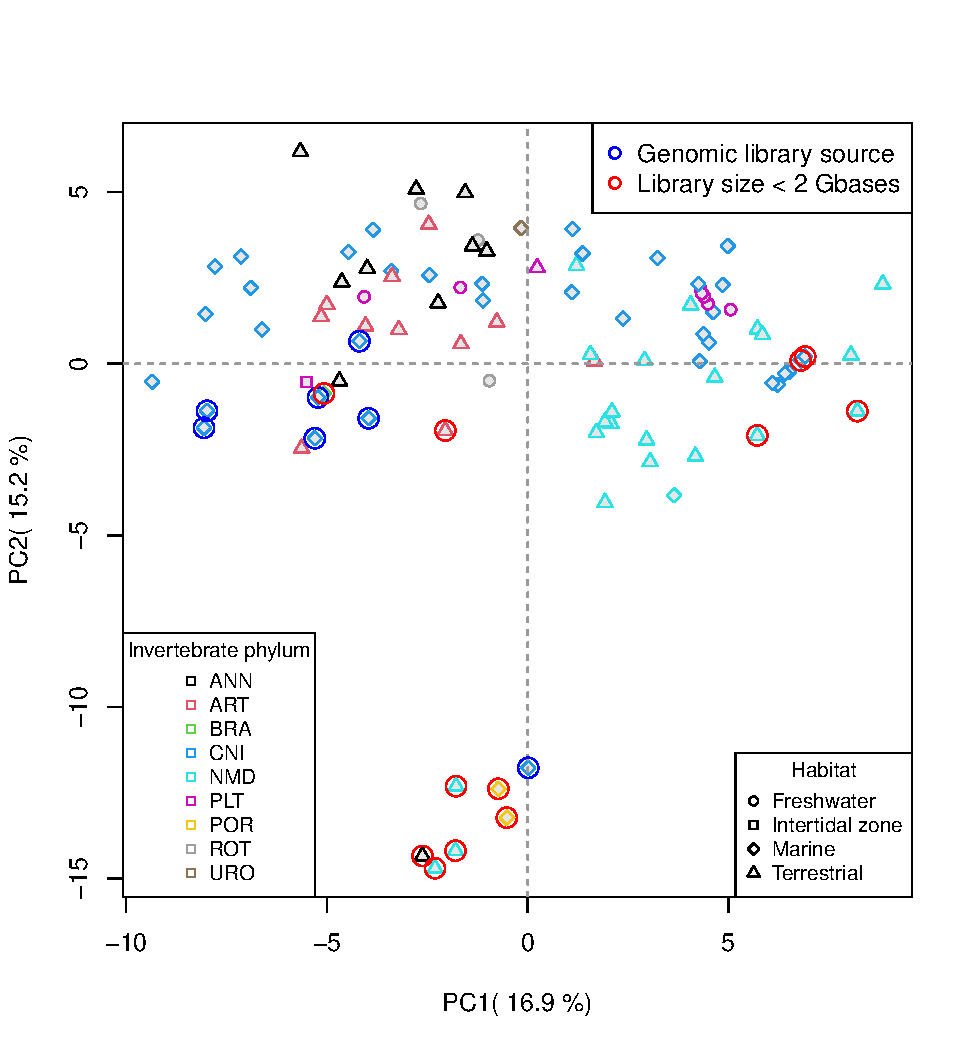
\includegraphics{_main_files/figure-latex/unnamed-chunk-20-1.pdf}

\caption{Scores plot for Kaiju PCA results before removing bias sources (Pilot).\label{fig:sample50biases}}
PC2 seems to separate a cluster of seven observations from the rest of the samples. These outlying observations have either a very low library size or a genomic rather than a transcriptomic library source, suggesting that both of these variables have a potentially notable effect on virome composition.
\end{figure}

\begin{figure}[!htbp]

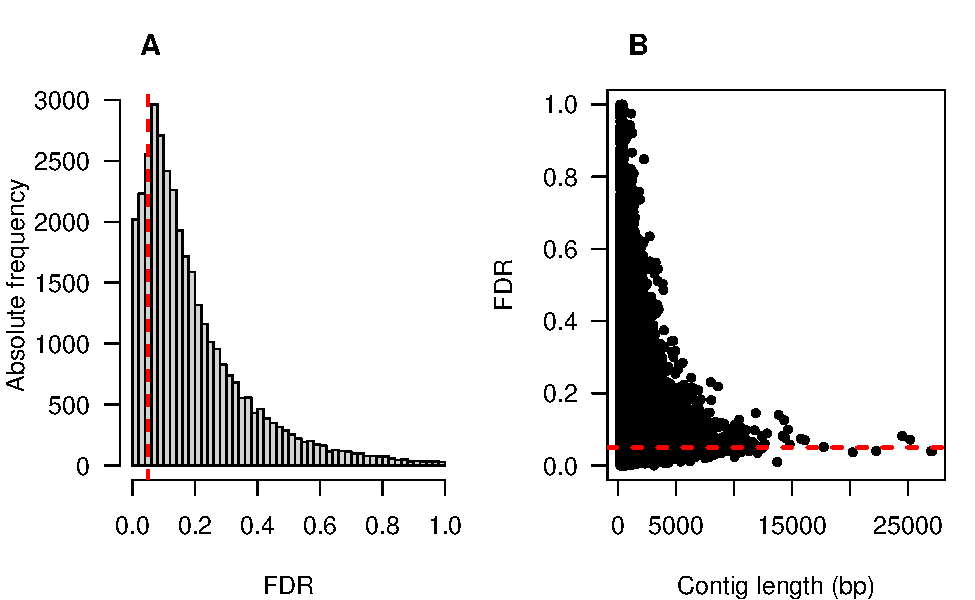
\includegraphics{_main_files/figure-latex/unnamed-chunk-21-1.pdf}

\caption{Overview of the distribution of $p$-values obtained by VirFinder (Pilot).\label{fig:vfpvals}}
$5000$ contig classification tests of seven accessions were randomly sampled to achieve an overview of the empirical distribution of their adjusted $p$-values ($FDR$). \textbf{A.} The histogram shows the predominance of small $FDR$ around the established significance threshold and the low proportion of $FDR$ in the upper half of their theoretical range. \textbf{B.} All observed $FDR$ near to 1 are observed for small contigs. As contig lengths increase, one could expect smaller $p$-values for true viral contigs and an uniform distribution [0,1] of $p$-values for non-viral contigs. 

\end{figure}

\begin{figure}[!htbp]

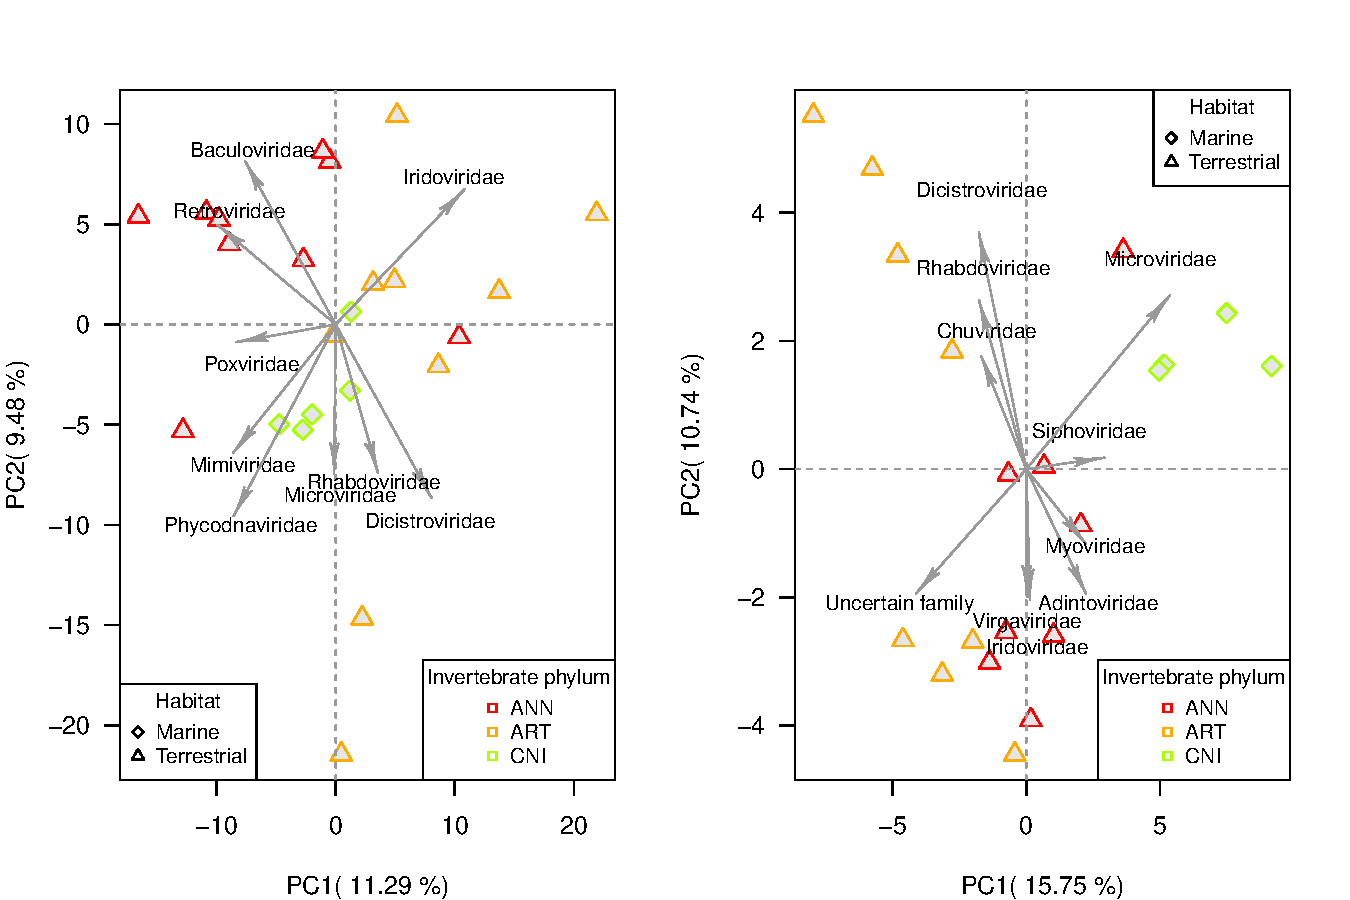
\includegraphics{_main_files/figure-latex/unnamed-chunk-22-1.pdf}

\caption{Biplot representation for PCA of VirFinder and VirSorter2 results (Pilot).\label{fig:sample50pcavfvs2}}
The contigs predicted to be viral according to VirFinder and VirSorter2 models were taxonomically classified into viral families using DIAMOND blastx. Both programs greatly differ in the average proportion of contigs considered viral, with VirSorter2 being much more conservative than VirFinder. \textbf{A.} Biplot of VirFinder PCA results does not reproduce what was seen in the straight DIAMOND analysis, since groups are more scattered and cnidarians lie in between annelids and arthropods, thus bluring out the habitat distinction of viromes. \textbf{B.} VirSorter2 reduced subset of contigs is enough to obtain similar conclusions to the DIAMOND analysis over the full set of contigs, since the distribution of scores and loadings is fairly similar, although higher within-group variation is noted. For both biplots, loadings vectors of most influential viral families for PC1 and PC2 are displayed. The scale of loadings does not correspond with the values on the axes and interpretations must be made in relative terms.
\end{figure}

\begin{figure}[!htbp]

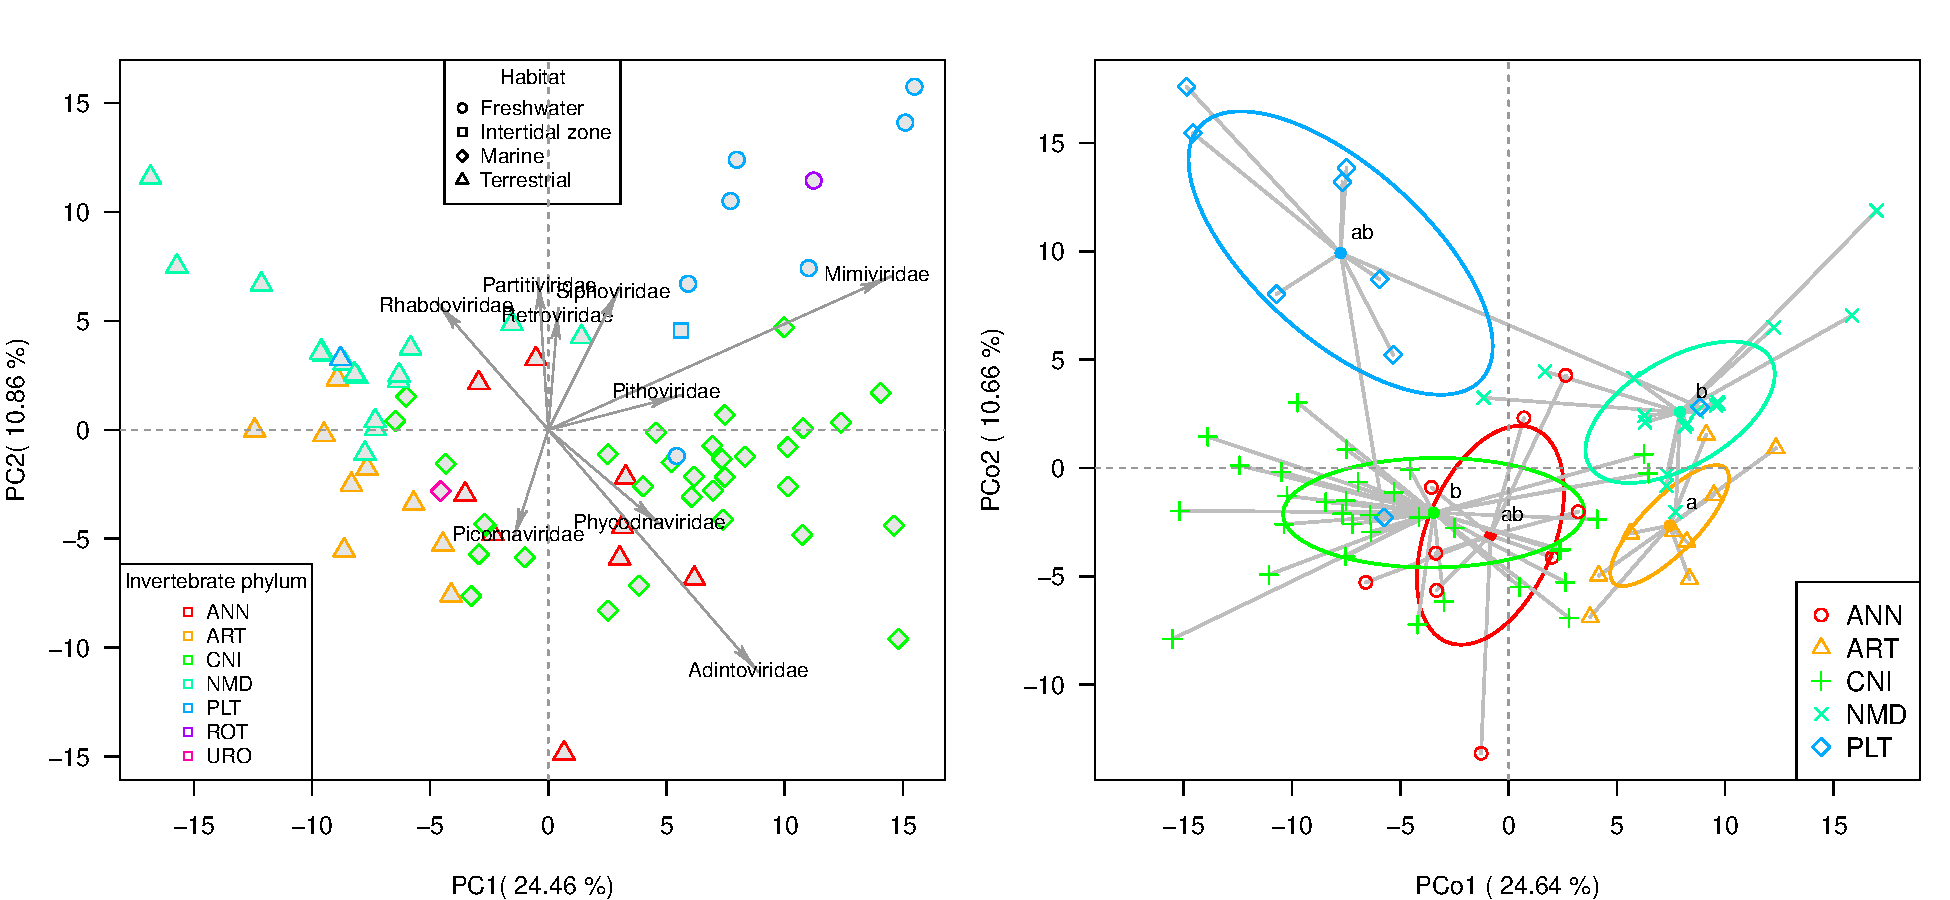
\includegraphics{_main_files/figure-latex/unnamed-chunk-23-1.pdf}

\caption{Multivariate exploratory analyses of CAT results (Pilot).\label{fig:sample50pcacat}}
\textbf{A.} PCA biplot was performed over CAT $clr$-transformed results after filtering DNA and low sequencing depth experiments. \textbf{B.} Rotifera and Urochordata groups were excluded for having only one observation each. Similar to what was observed for PERMANOVA results with DIAMOND data, invertebrate phylum distinction of the samples originates significant differences in location and/or dispersion ($P < 0.05$) and is able to explain roughly $30\%$ of the variance in the Aitchison distances matrix. PERMDISP test shows that there are differences in dispersion between phyla ($P < 0.05$). Groupings of phyla according to their dispersion were determined by Tukey test: arthropods seem to have the most uniform viromes and cnidarians and nematodes the most diverse.
\end{figure}

\begin{figure}[!htbp]

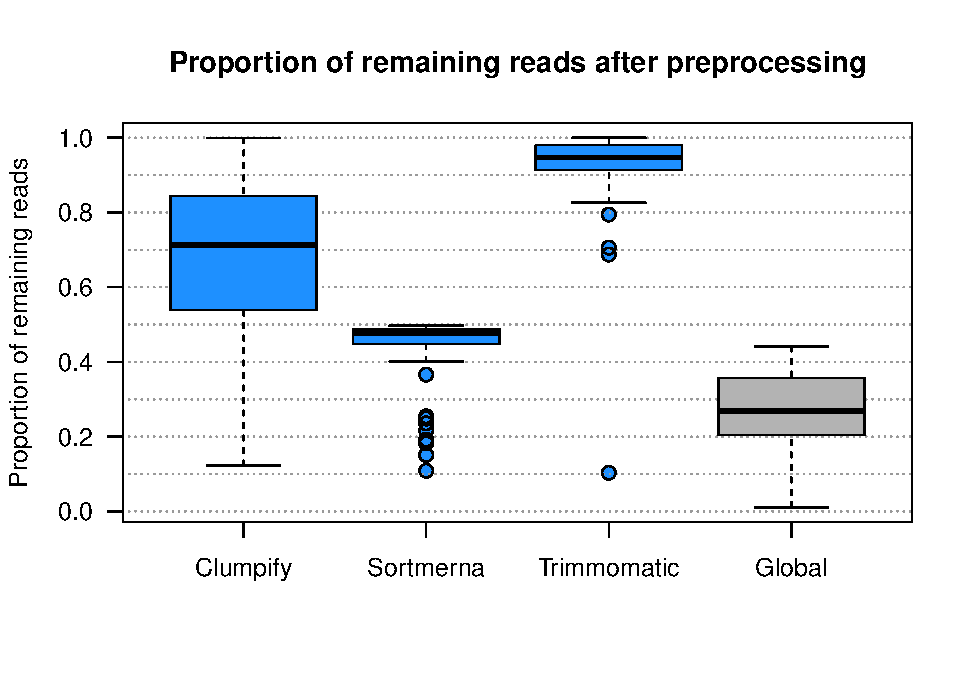
\includegraphics{_main_files/figure-latex/unnamed-chunk-24-1.pdf}

\caption{Proportion of reads preserved after each preprocessing step of the definitive pipeline.\label{fig:preprocess}}
Each preprocessing step is evaluated over the subset of reads left after the previous steps: while Clumpify performs deduplication on the original set of raw reads, removal of reads with SortMeRNA is relative to the subset of reads without duplicates. The reported proportion of remaining reads for Trimmomatic refers to the subset of reads preserved after Clumpify and SortMeRNA. The distribution of the global proportion of reads left after the whole preprocessing is displayed in grey in the figure.
\end{figure}

\begin{figure}[!htbp]

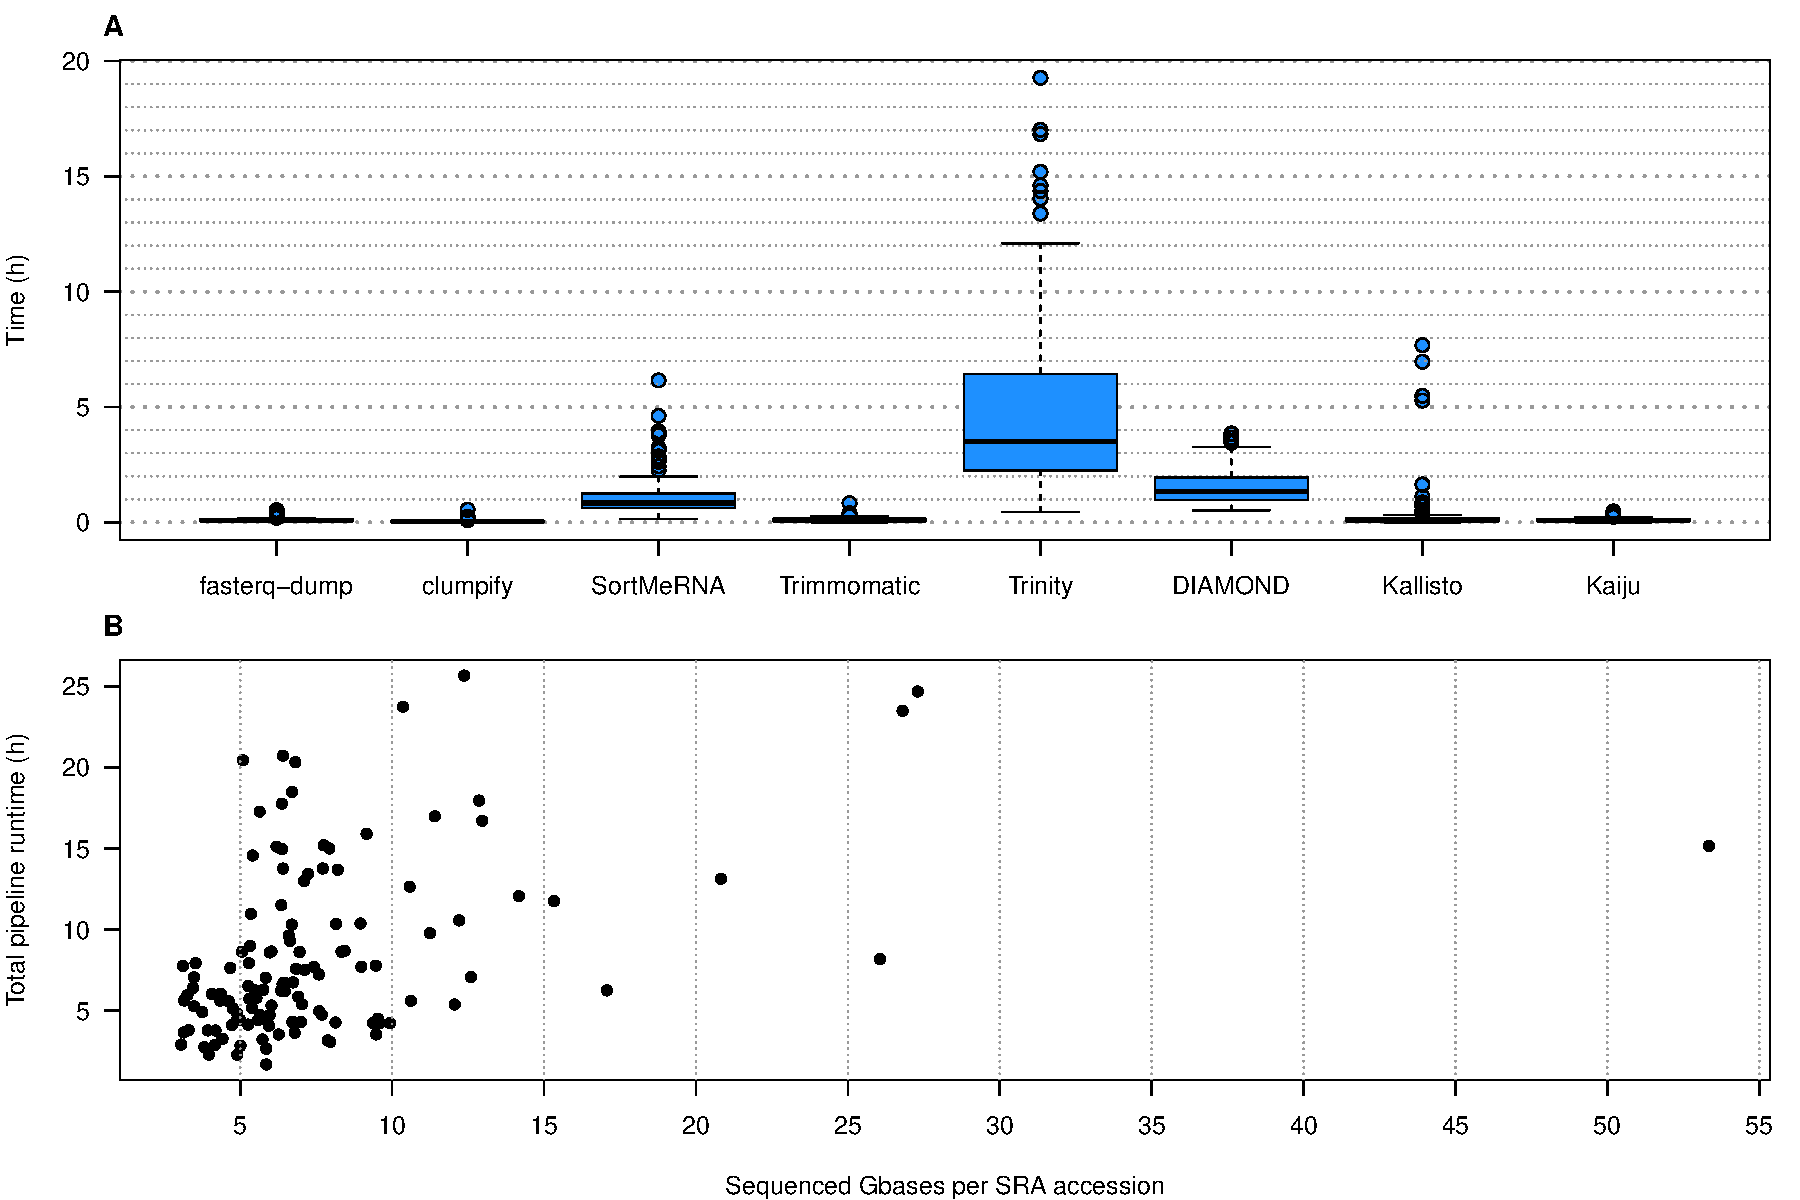
\includegraphics{_main_files/figure-latex/unnamed-chunk-25-1.pdf}

\caption{Distribution of runtimes in the definitive pipeline.\label{fig:pipelinetimes}}
\textbf{A.} Time elapsed in hours by each program in the order of the pipeline. The fact that distributions are positively skewed is likely due to overload in the HPC task manager (slurm) and the presence of accessions with particularly large library sizes. \emph{De novo} assembly constitutes the slowest step, although a noticeable filtering of reads was performed in the preprocessing. \textbf{B.} The total processing time of the accessions is positively related to their library sizes. $50\%$ of central individuals in the distribution of library sizes have between 5 to 8 Gb sequenced.
\end{figure}

\begin{figure}[!htbp]

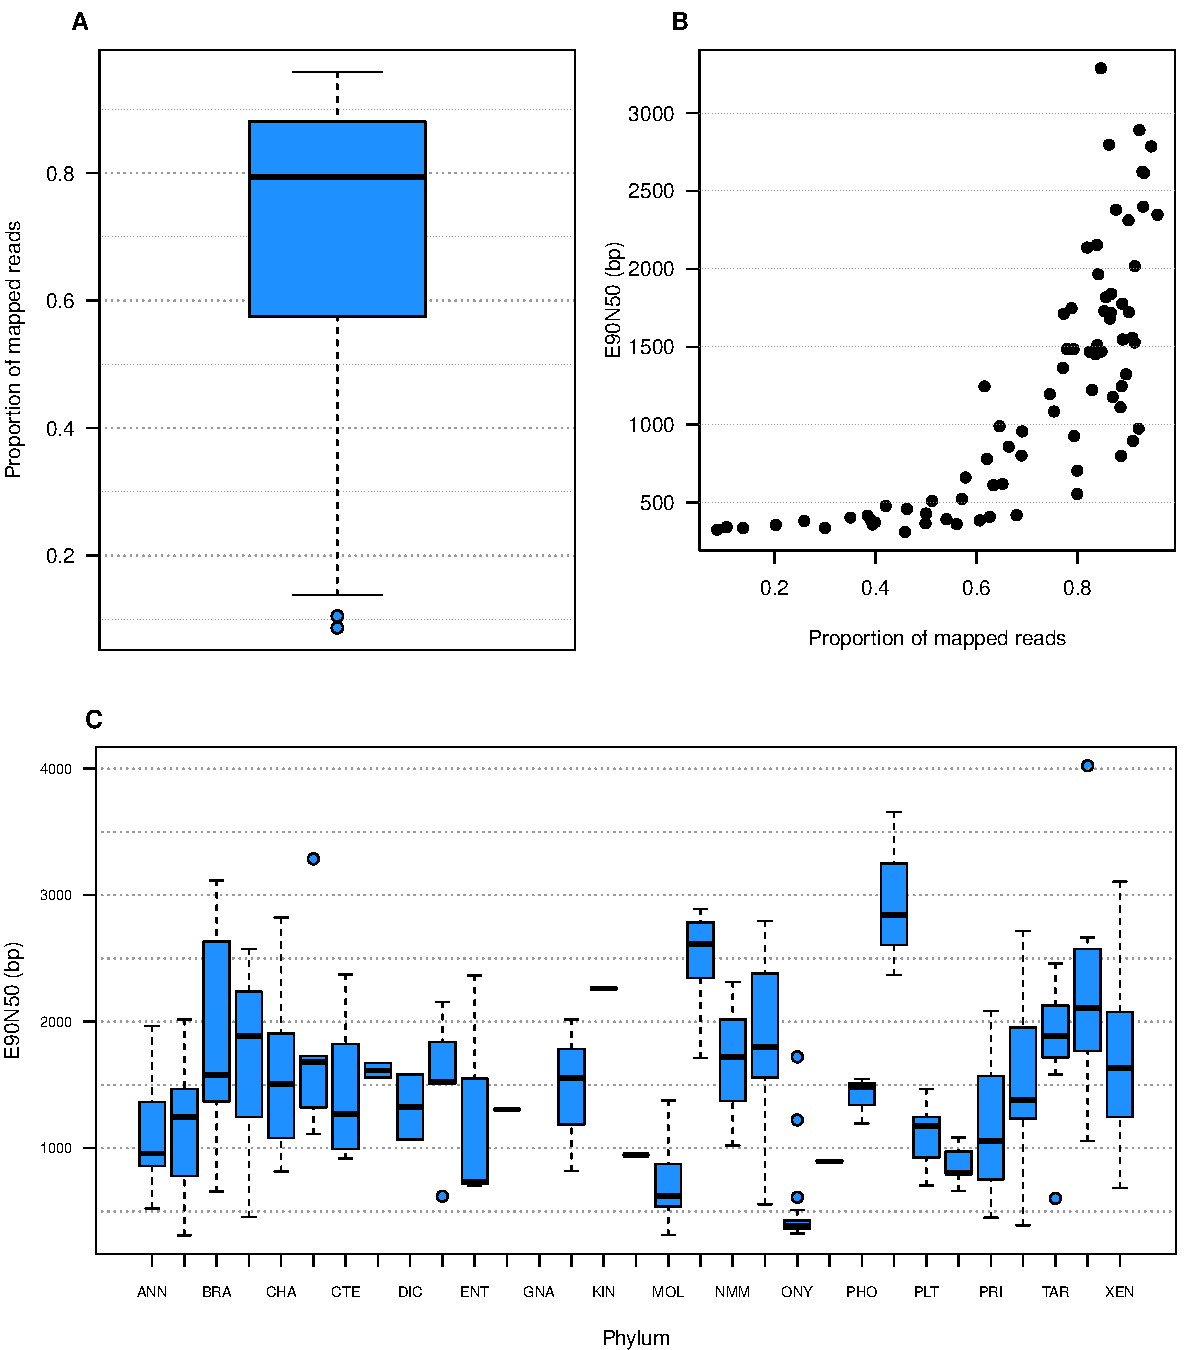
\includegraphics{_main_files/figure-latex/unnamed-chunk-26-1.pdf}

\caption{Overview of assembly statistics in the definitive analysis.\label{fig:assemblystats}}
\textbf{A.} Proportion of reads left after Trimmomatic that were mapped into contigs with Trinity. \textbf{B.} Assemblies that arise from a low proportion of reads tend to form contigs of lower length and thus, assemblies of lower quality. \textbf{C.} Quality of assemblies is not uniformly distributed among samples of different invertebrate phyla. This could be due to either experimental or biological reasons. Interestingly enough, this is not an artifact of library sizes, which are distributed similarly among phyla.
\end{figure}

\begin{figure}[!htbp]

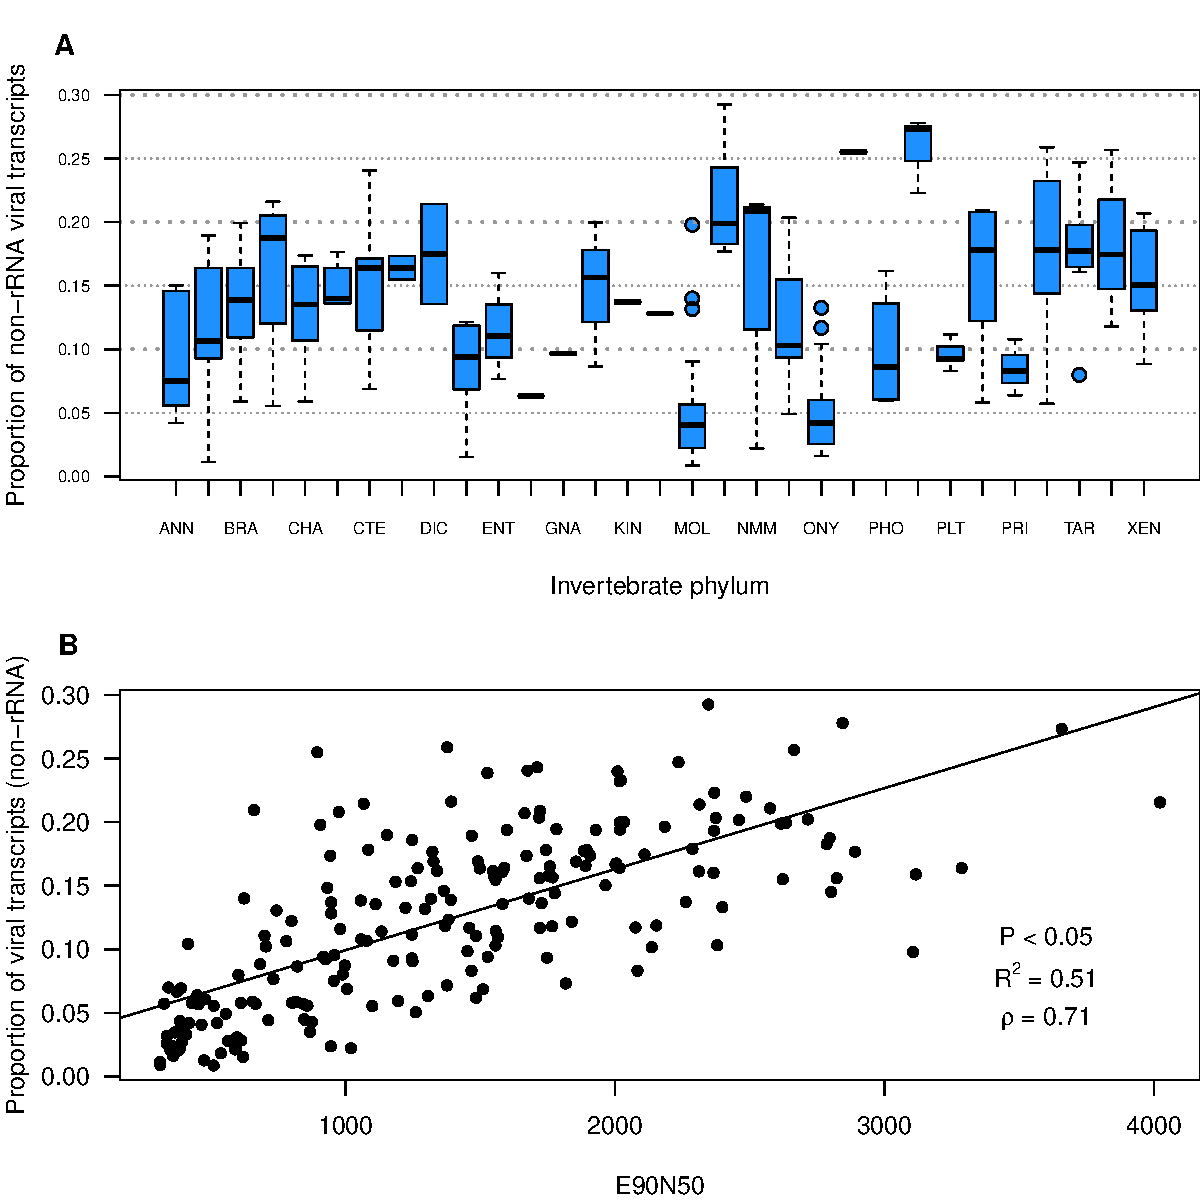
\includegraphics{_main_files/figure-latex/unnamed-chunk-27-1.pdf}

\caption{Distribution of the proportion of viral transcripts in DIAMOND results.\label{fig:virqual}}
\textbf{A.} The concentration of viral transcripts in the non-rRNA, non-COX transcriptome in a similar way to E90N50 across phyla in the sampled observations. For instance, Onychophora shows very low virus transcript concentrations while Placozoa shows much higher ones. \textbf{B.} A simple linear regression model fits the relationship between total virus abundance and E90N50 relatively well.


\end{figure}

\begin{figure}[!htbp]

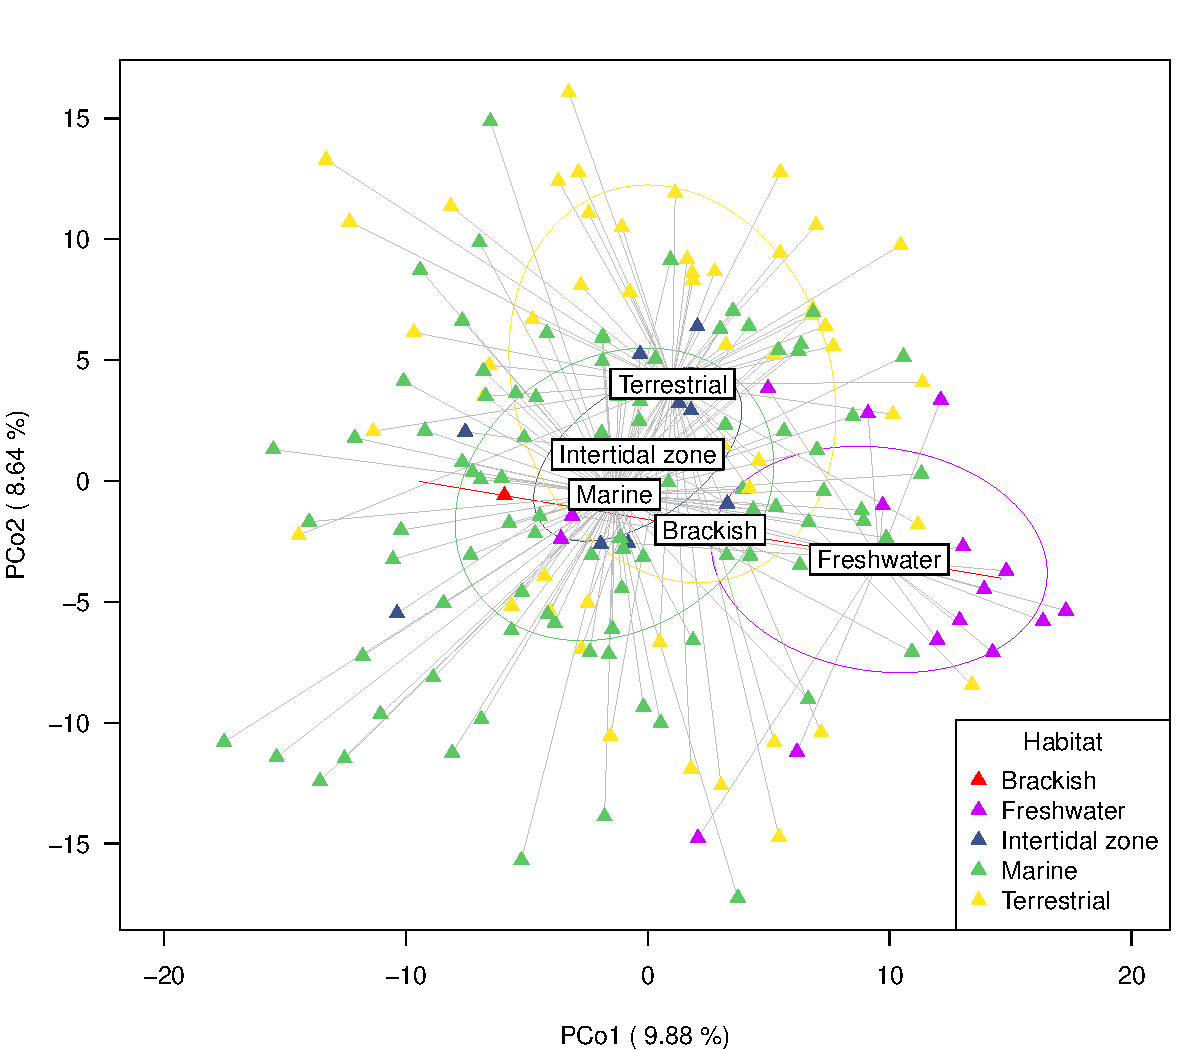
\includegraphics{_main_files/figure-latex/unnamed-chunk-28-1.pdf}

\caption{PCoA over the Aitchison distances matrix of DIAMOND results.\label{fig:habpcoa}}
PCoA was performed over the Aitchison distances of the $209\times54$ compositional matrix with observations of the 18 most abundant phyla. Two first principal coordinates are able to explain roughly $19\%$ of the variance. Freshwater viromes are the most divergent from the rest in terms of composition. Apparently, they are similarly distant to terrestrial and marine viromes, whose centroids lie closer to each other.

\end{figure}

\begin{figure}[!htbp]

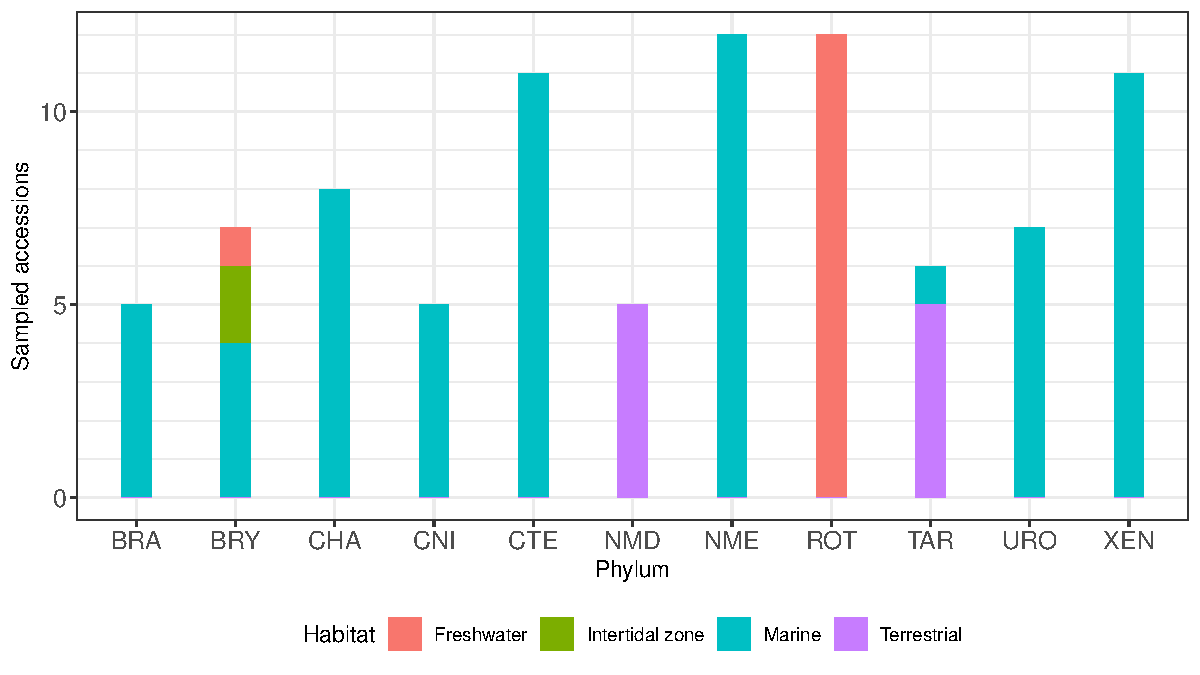
\includegraphics{_main_files/figure-latex/unnamed-chunk-29-1.pdf}

\caption{Distribution of habitats within phyla for the subset of high quality assemblies.\label{fig:qualdiver}}
Only phyla with more than four associated accessions remaining are displayed in the figure.


\end{figure}

\begin{figure}[!htbp]

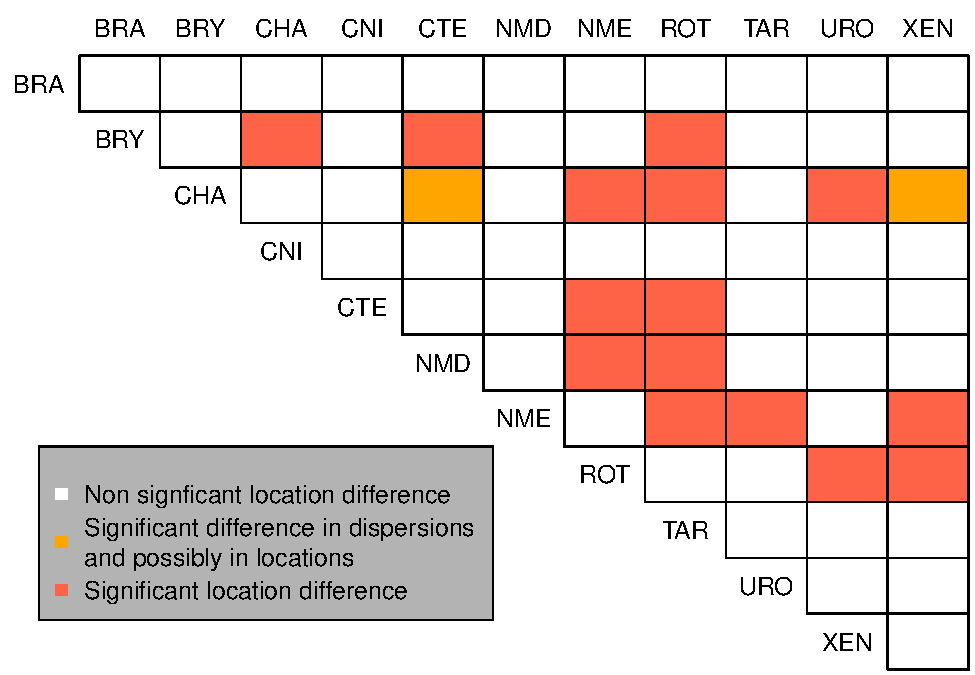
\includegraphics{_main_files/figure-latex/unnamed-chunk-30-1.pdf}

\caption{Results of pairwise PERMANOVA and PERMDISP tests on the subset of high quality assemblies.\label{fig:permmatrix}}
The results of the PERMANOVA and PERMDISP tests for each combination of phyla are encoded in its respective cell of the matrix. $p$-values were corrected by $FDR$ method. For a particular combination, if only PERMANOVA yields an adjusted $p$-value lower than $0.05$, significant differences in location are accepted (red). If also PERMDISP yields an adjusted $p$-value lower than 0.05, heterogeneity of dispersions exist between the phyla and the actual location differences are uncertain (orange). In this case, none of the combinations was associated with only a rejection of $H_0$ in PERMDISP. Combinations where no significant differences are found for any of the two tests, such as in the diagonal, are illustrated with white cells. Only the upper triangle of the matrix is shown to avoid redundancy.

\end{figure}

\begin{figure}[!htbp]

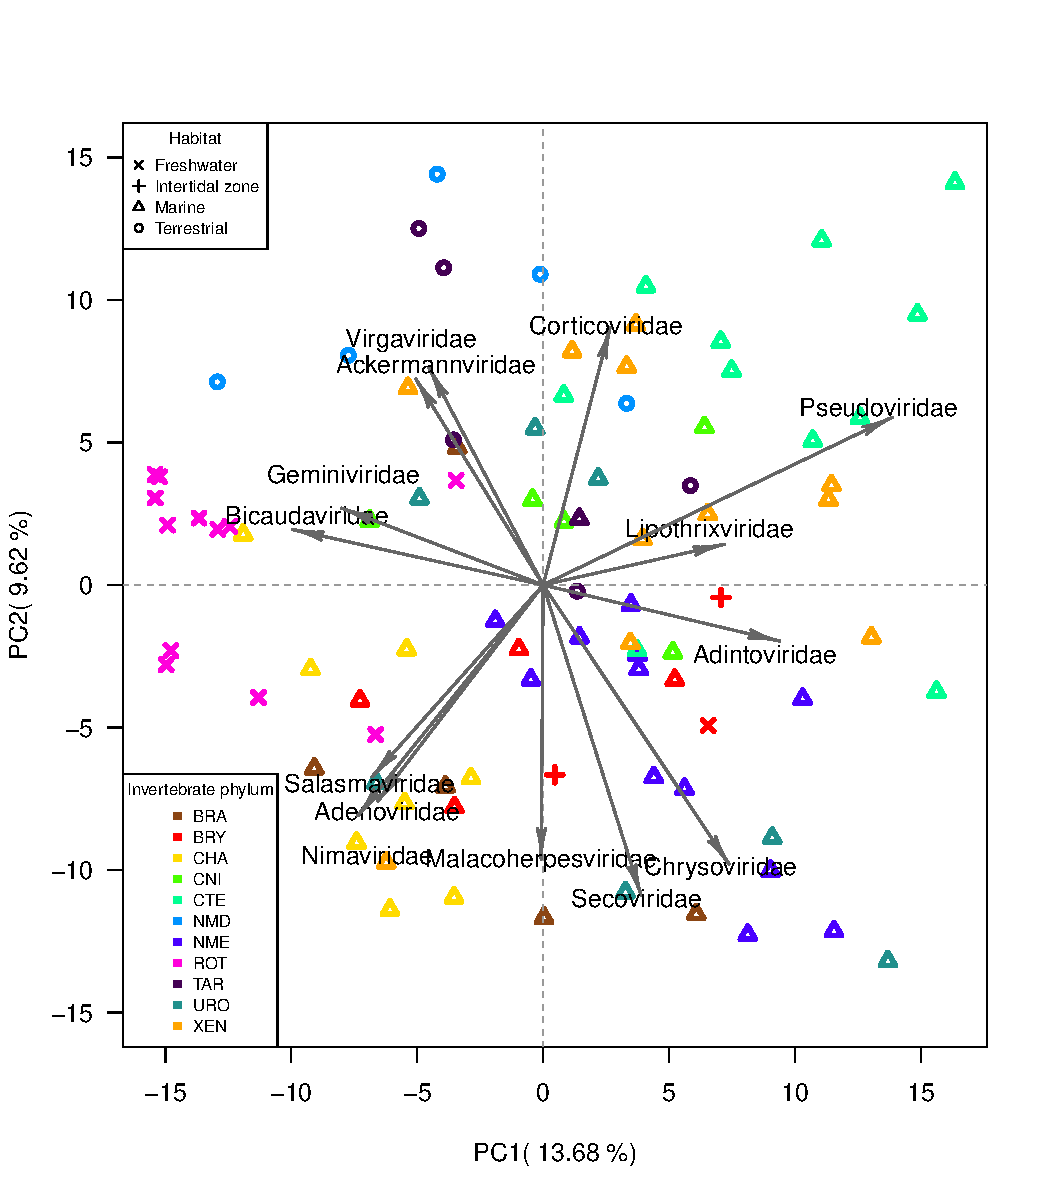
\includegraphics{_main_files/figure-latex/unnamed-chunk-31-1.pdf}

\caption{PCA biplot of virome compositions estimated with DIAMOND in the subset of high quality assemblies.\label{fig:pcaqual}}
SVD was performed over the $89 \times 52$ matrix of \emph{clr} coefficients. Loadings vectors that are greater in absolute value than $0.2$ in any of the first two PC are shown. Loadings vectors are rescaled to improve their readability. Percentage of variance explained by each orthogonal PC dimension is displayed in its respective axis.

\end{figure}

\printbibliography

\end{document}
